%
%%%%%%%%%%%%%%%%%%%%%%%%%%%%%%%%%%%%%%%%%%%%%%%%%%%%%%%%%%%%%%%%%%%%%%%%%%%%%%%
\chapter{The Multivariate Analysis}\label{ch:mva}
%%%%%%%%%%%%%%%%%%%%%%%%%%%%%%%%%%%%%%%%%%%%%%%%%%%%%%%%%%%%%%%%%%%%%%%%%%%%%%%
%

Multivariate technique
multivariate classification
learning algorithms
They make use of training events, for which the desired output is known, to determine the mapping function that discribes a decision boundary (classification)


%------------------------------------------------------------------------
%\section{The multivariate classifiers}
%------------------------------------------------------------------------

The following multivariate methods were explored:

\begin{itemize}\addtolength{\itemsep}{-0.4\baselineskip}
\item
Likelihood ratio estimators 
\item
Neural Networks (NN)
\item
Boosted decision Trees (BDTs)
\item
Fisher discriminants
\end{itemize}

%From TMVA Users Guide
The method of maximum likelihood consists of building a model out of probability density functions (PDF) that reproduces the input variables for signal and background. For a given event, the likelihood for being of signal type is obtained by multiplying the signal probability densities of all input variables %, which are assumed to be independent, 
and normalising this by the sum of the signal and background likelihoods. %Because correlations among the variables are ignored, this PDE approach is also called “naive Bayes estimator”.
The likelihood ratio $y_{L}(i)$ for event $i$ is defined by:
%
\begin{equation}
y_{L}(i) = \frac{L_S(i)}{L_S(i)+L_B(i)},
\end{equation}
%
where
%
\begin{equation}
L_{s(B)}(i) = \prod^{n_{var}}_{k=1}  p_{s(B),k}(x_k(i)),
\end{equation}
%
and where $p_{s(B),k}(x_k(i))$ is the signal (background) PDF for the $k$th input variable $x_k$. All the PDFs are normalized to one. 

The parametric form of the PDFs is generally unknown, however it is possible to empirically approximate its shape from the training data by nonparametric functions  which can be chosen individually for each variable and are either polynomial splines of various degrees fitted to binned histograms or unbinned kernel density estimators (KDE).
%From wikipedia SPLINES
%In mathematics, a spline is a sufficiently smooth polynomial function that is piecewise-defined, and possesses a high degree of smoothness at the places where the polynomial pieces connect (which are known as knots).
%In interpolating problems, spline interpolation is often referred to as polynomial interpolation because it yields similar results,
%From wikipedia NON-PARAMETRIC METHODS
%Non-parametric models differ from parametric models in that the model structure is not specified a priori but is instead determined from data. The term non-parametric is not meant to imply that such models completely lack parameters but that the number and nature of the parameters are flexible and not fixed in advance.
%A histogram is a simple nonparametric estimate of a probability distribution
% Kernel density estimation provides better estimates of the density than histograms.
%In statistics, kernel density estimation (KDE) is a non-parametric way to estimate the probability density function of a random variable. Kernel density estimation is a fundamental data smoothing problem where inferences about the population are made, based on a finite data sample.
%Kernel density estimates are closely related to histograms, but can be endowed with properties such as smoothness or continuity by using a suitable kernel.
%The smoothness of the kernel density estimate is evident compared to the discreteness of the histogram, as kernel density estimates converge faster to the true underlying density for continuous random variables.


Both the training and the application of the likelihood are very fast operations that are suitable for very large data sets. %The neglect of correlations between input variables in the model, often leads to a diminution of the discrimination performance. Positive correlations lead to peaks at both yL → 0, 1. Correlations can be reduced by categorising the data samples and building an independent likelihood classifier for each event category. Such categories could be geometrical regions in the detector, kinematic properties, etc.


%From TMVA Users Guide

The method of Fisher discriminants~\cite{Fisher}.

An artificial Neural Network (NN) is a nonlinear discriminant, it is most generally speaking any simulated collection of interconnected neurons, with each neuron producing a certain response at a given set of input signals.
. It can be viewed as a mapping from a space of input variables $x_1,...,x_n_{var}$ onto, in the case of a signal-versus-background discimination problem, a one-dimensional output variable. The behaviour of an artificial neural network is determined by the layout of the neurons, the weights of the inter-neuron connections, and by the response of the neurons to the input, described by the neuron response function ρ.
While in principle a neural network with $n$ neurons can have $n^2$ directional connections, the complexity can be reduced by organising the neurons in layers and only allowing direct connections from a given layer to the following layer. This kind of neural network is termed multi-layer perceptron. The first layer of a multilayer perceptron is the input layer, the last one the output layer, and all others are hidden layers. For a classification problem with nvar input variables the input layer consists of $n_{var}$ neurons that hold the input values, $x_1,...,x_n_{var}$, and one neuron in the output layer that holds the output variable, the neural net estimator $y_{ANN}$ .
%The neuron response function ρ maps the neuron input i1 , . . . , in onto the neuron output (Fig. 16). Often it can be separated into a Rn → R synapse function κ, and a R → R neuron activation function α, so that ρ = α ◦ κ


The NN used were built with only one hidden layer. %When building a network two rules should be kept in mind. The first is the theorem by Weierstrass, which if applied to neural nets, ascertains that for a multilayer perceptron a single hidden layer is  sufficient to approximate a given continuous correlation function to any precision, provided that a sufficiently large number of neurons is used in the hidden layer. If the available computing power and the size of the training data sample suffice, one can increase the number of neurons in the hidden layer until the optimal performance is reached.


A decision tree (BDT)~\cite{QUINLAN1999497} is a binary tree structured classifier. Repeated yes/no decisions are taken on one single variable at a time until a stop criterion is fulfilled.  The phase space is split this way into many regions that are eventually classified as signal or background, depending on the majority of training events that end up in the final $leaf$ node. The boosting of a decision tree extends this concept from one tree to several trees which form a $forest$.
%Decision trees are well known classifiers that allow a straightforward interpretation as they can be visualized by a simple two-dimensional tree structure. They are in this respect similar to rectangular cuts. However, whereas a cut-based analysis is able to select only one hypercube as region of phase space, the decision tree is able to split the phase space into a large number of hypercubes, each of which is identified as either ``signal-like'' or ``background-like''.
%Boosting increases the statistical stability of the classifier and typically also improves the separation performance compared to a single decision tree. However, the advantage of the straightforward interpretation of the decision tree is lost.
%Decision trees are also insensitive to the inclusion of poorly discriminating input variables. While for artificial neural networks it is typically more difficult to deal with such additional variables, the decision tree training algorithm will basically ignore non-discriminating variables as for each node splitting only the best discriminating variable is used. 









%And different trainings were tested:
%\begin{itemize}\addtolength{\itemsep}{-0.4\baselineskip}
%\item
%Inclusive, with $\pt$-weighting
%\item
%In bins of jet $\pt$
%\end{itemize}
Figure~\ref{fig:diffmethodsInclusive} and~\ref{fig:diffmethodsBins} show distributions of the MVA outputs in different bins of jet $\pt$ for the two proposed trainings. In figures~\ref{fig:diffmethodsPerfInclusive} and~\ref{fig:diffmethodsPerfBins} a comparison of the performance of all methods, for inclusive and ``in-bins'', training is illustrated.


\begin{figure}[tp]
\centering
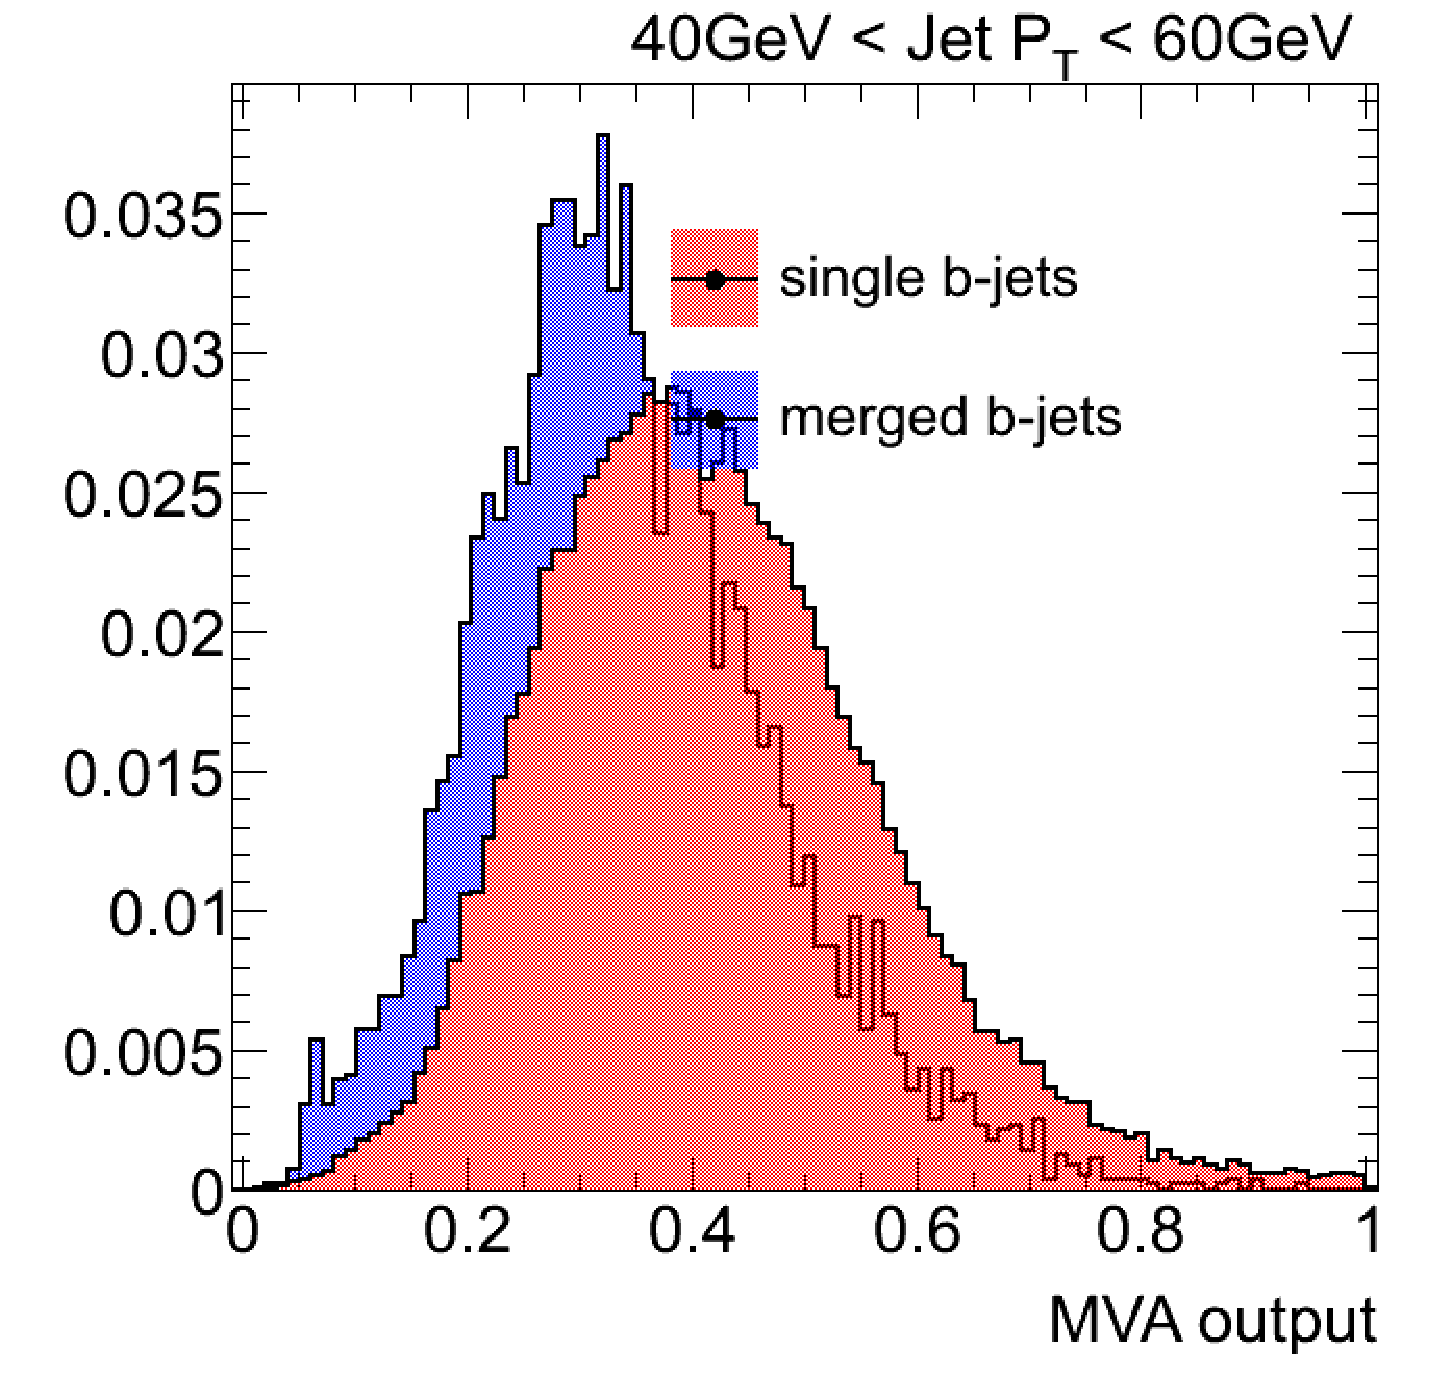
\includegraphics[width=0.32\textwidth]{FIGS/TEMPFigs/MVA_differentMethods/inclusive/NNoutput040_LihoodKDE.pdf}
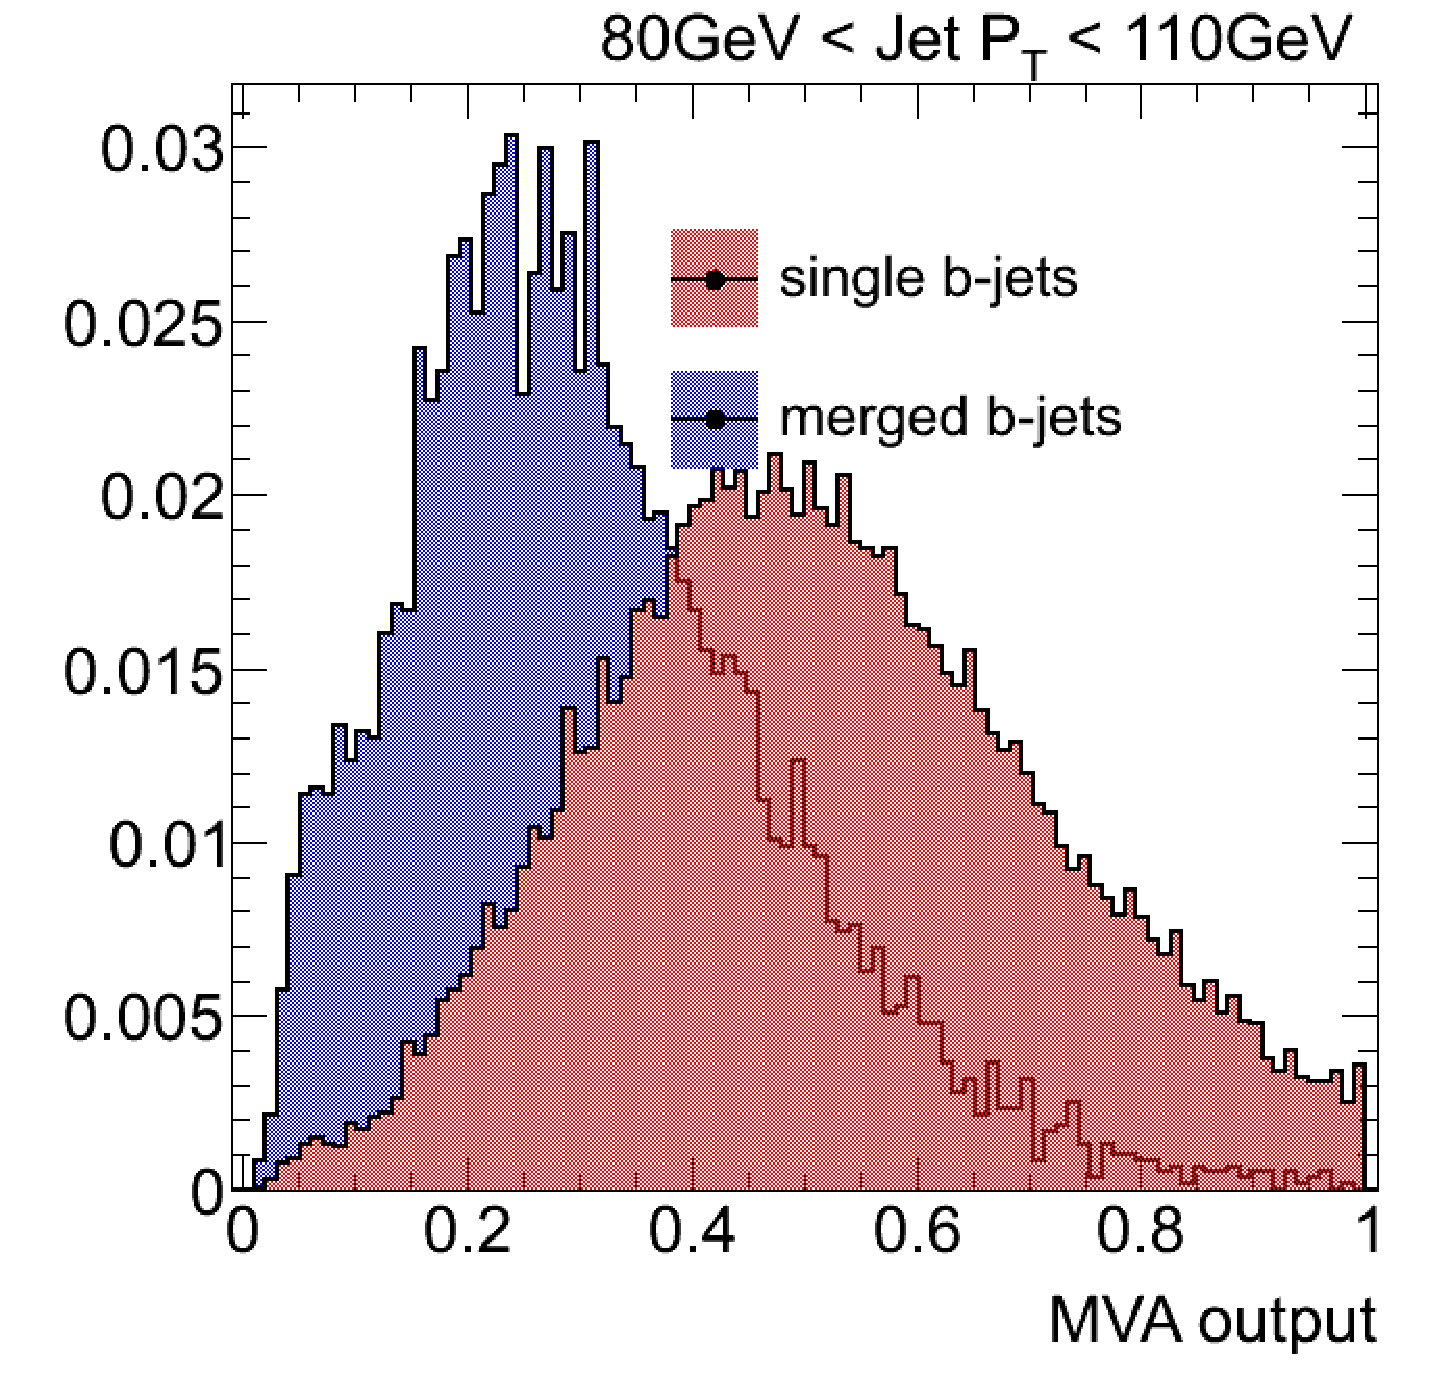
\includegraphics[width=0.32\textwidth]{FIGS/TEMPFigs/MVA_differentMethods/inclusive/NNoutput080_LihoodKDE.pdf}
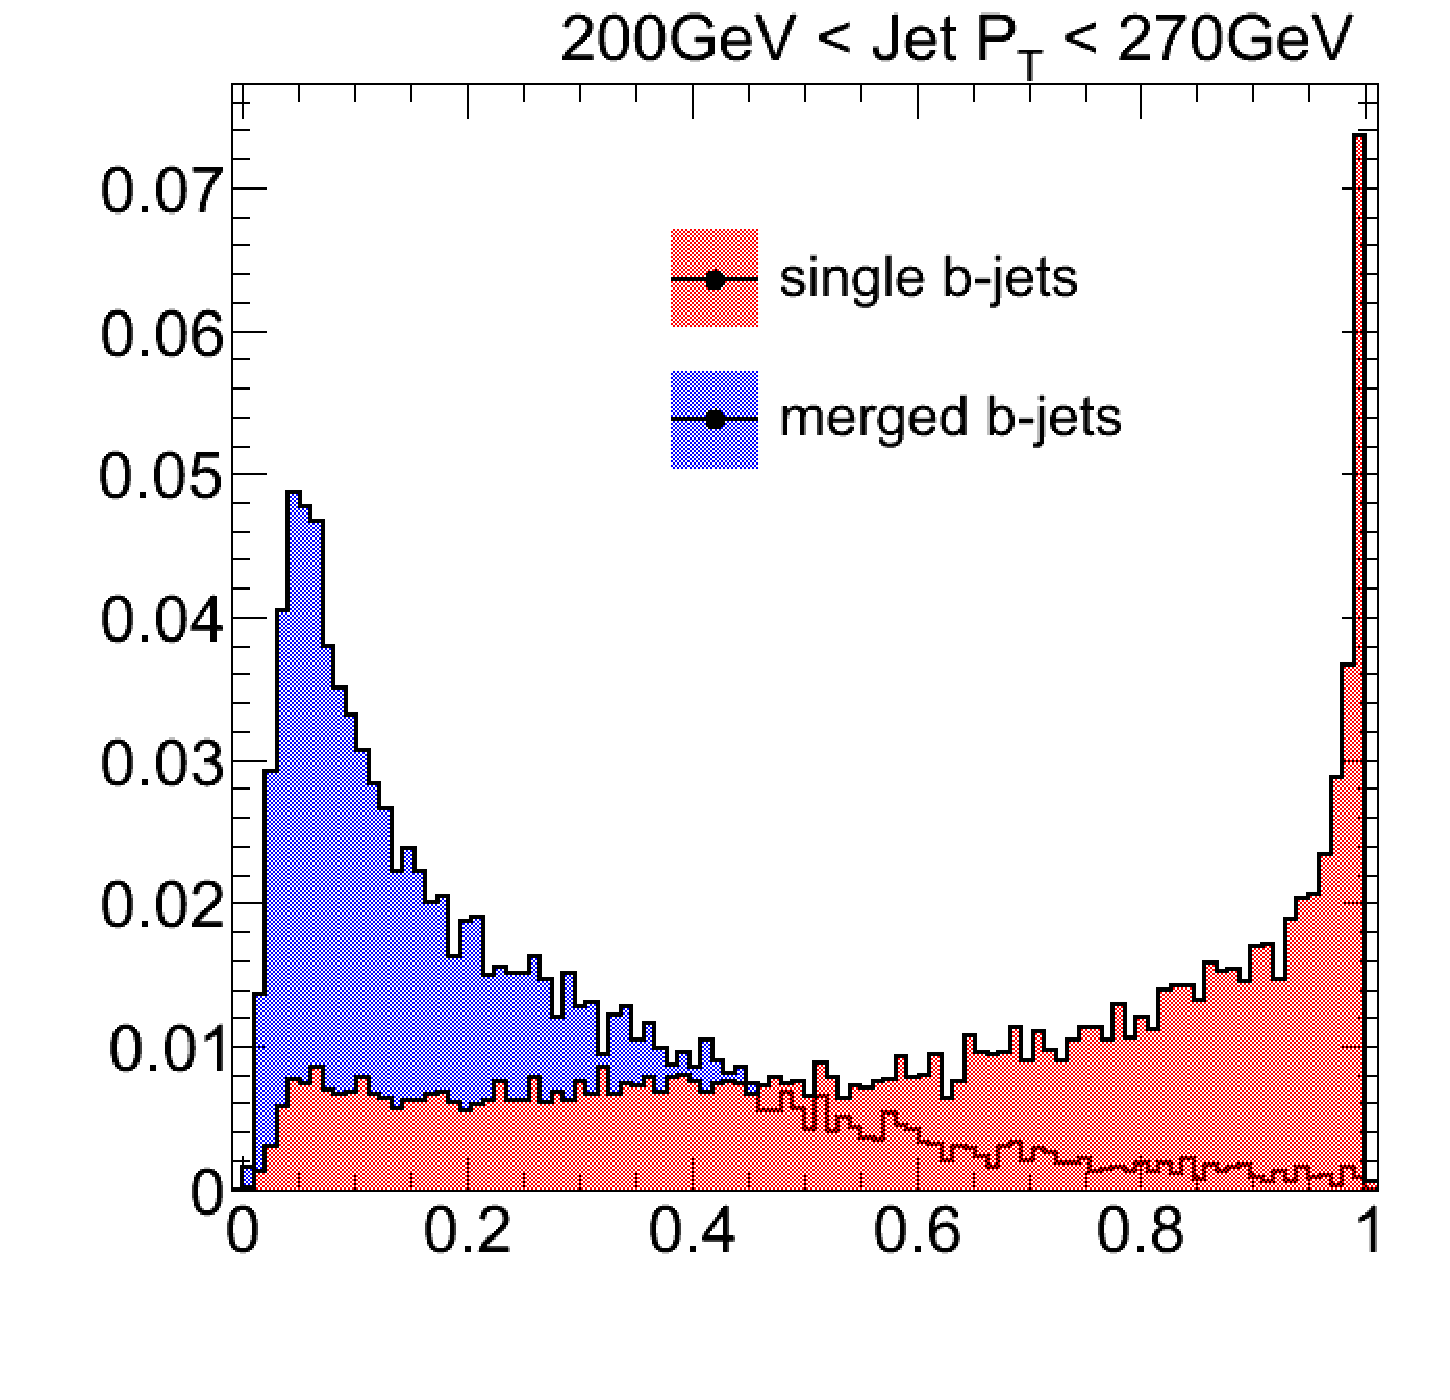
\includegraphics[width=0.32\textwidth]{FIGS/TEMPFigs/MVA_differentMethods/inclusive/NNoutput200_LihoodKDE.pdf}
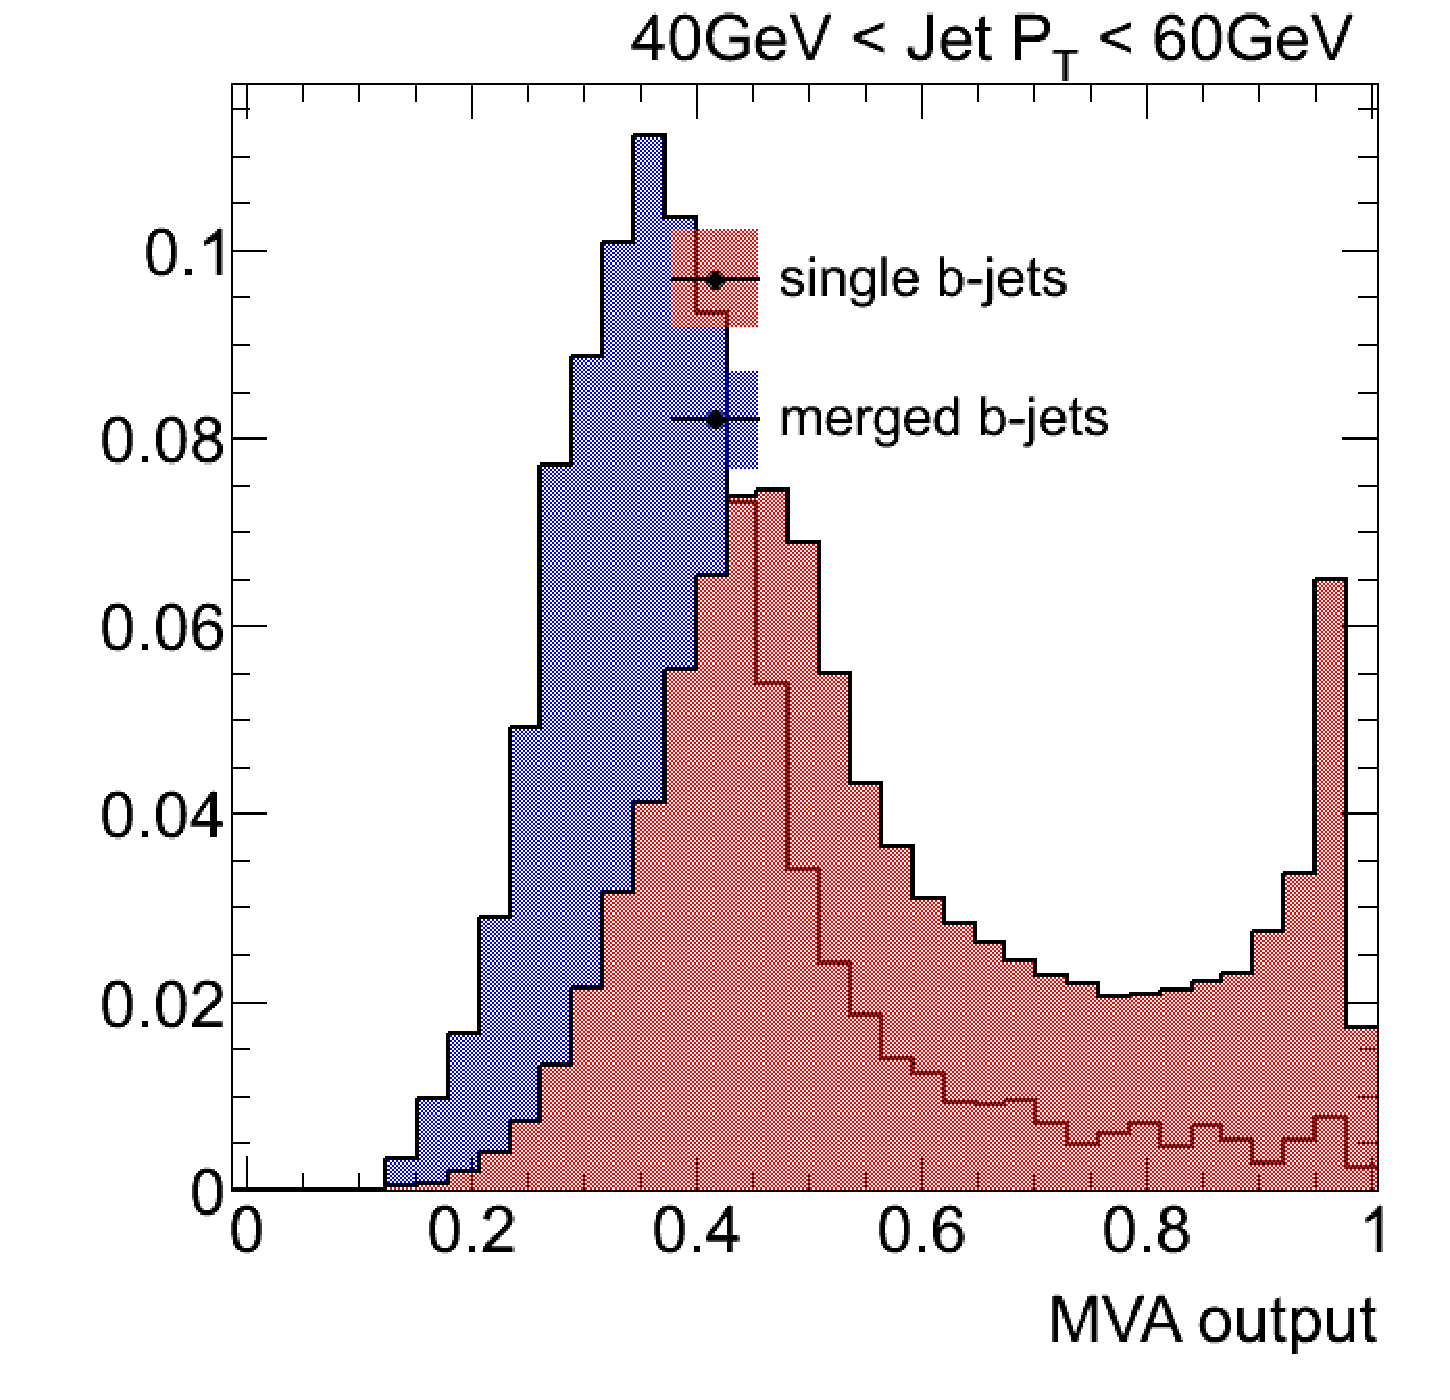
\includegraphics[width=0.32\textwidth]{FIGS/TEMPFigs/MVA_differentMethods/inclusive/NNoutput040_MLP.pdf}
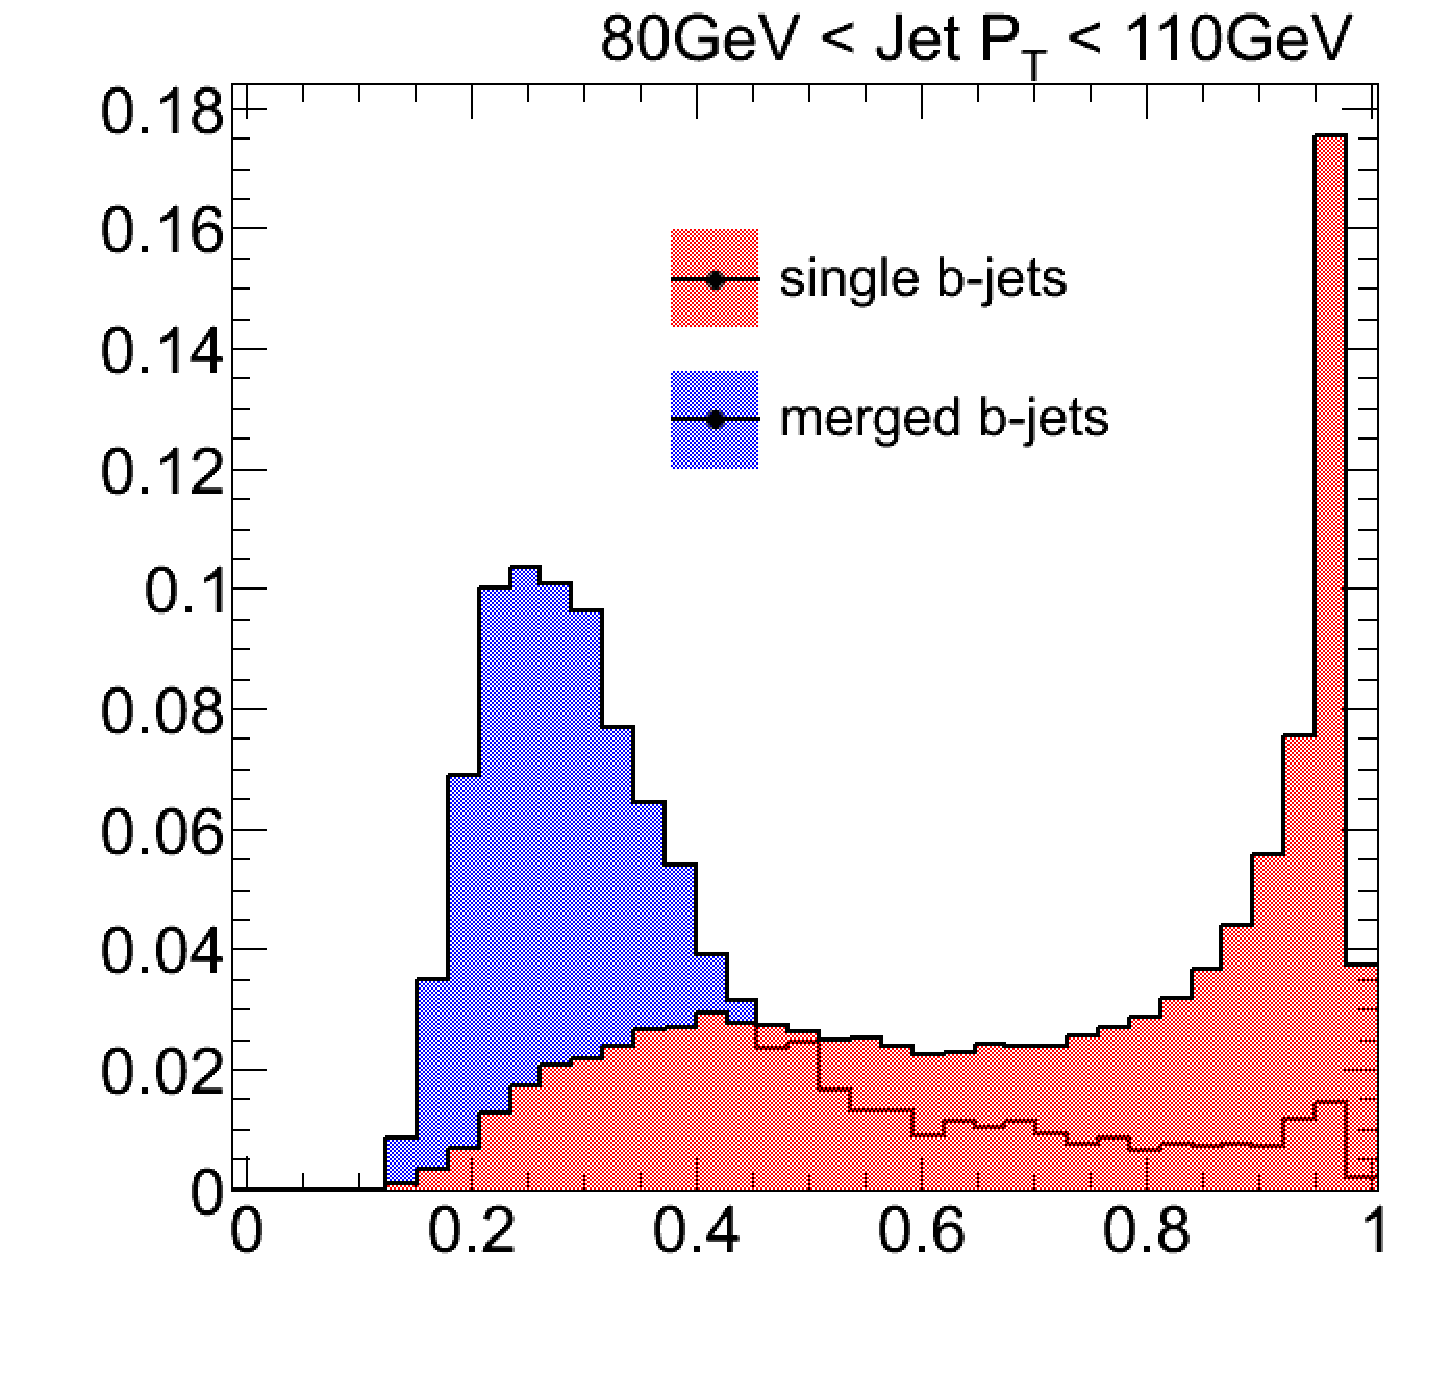
\includegraphics[width=0.32\textwidth]{FIGS/TEMPFigs/MVA_differentMethods/inclusive/NNoutput080_MLP.pdf}
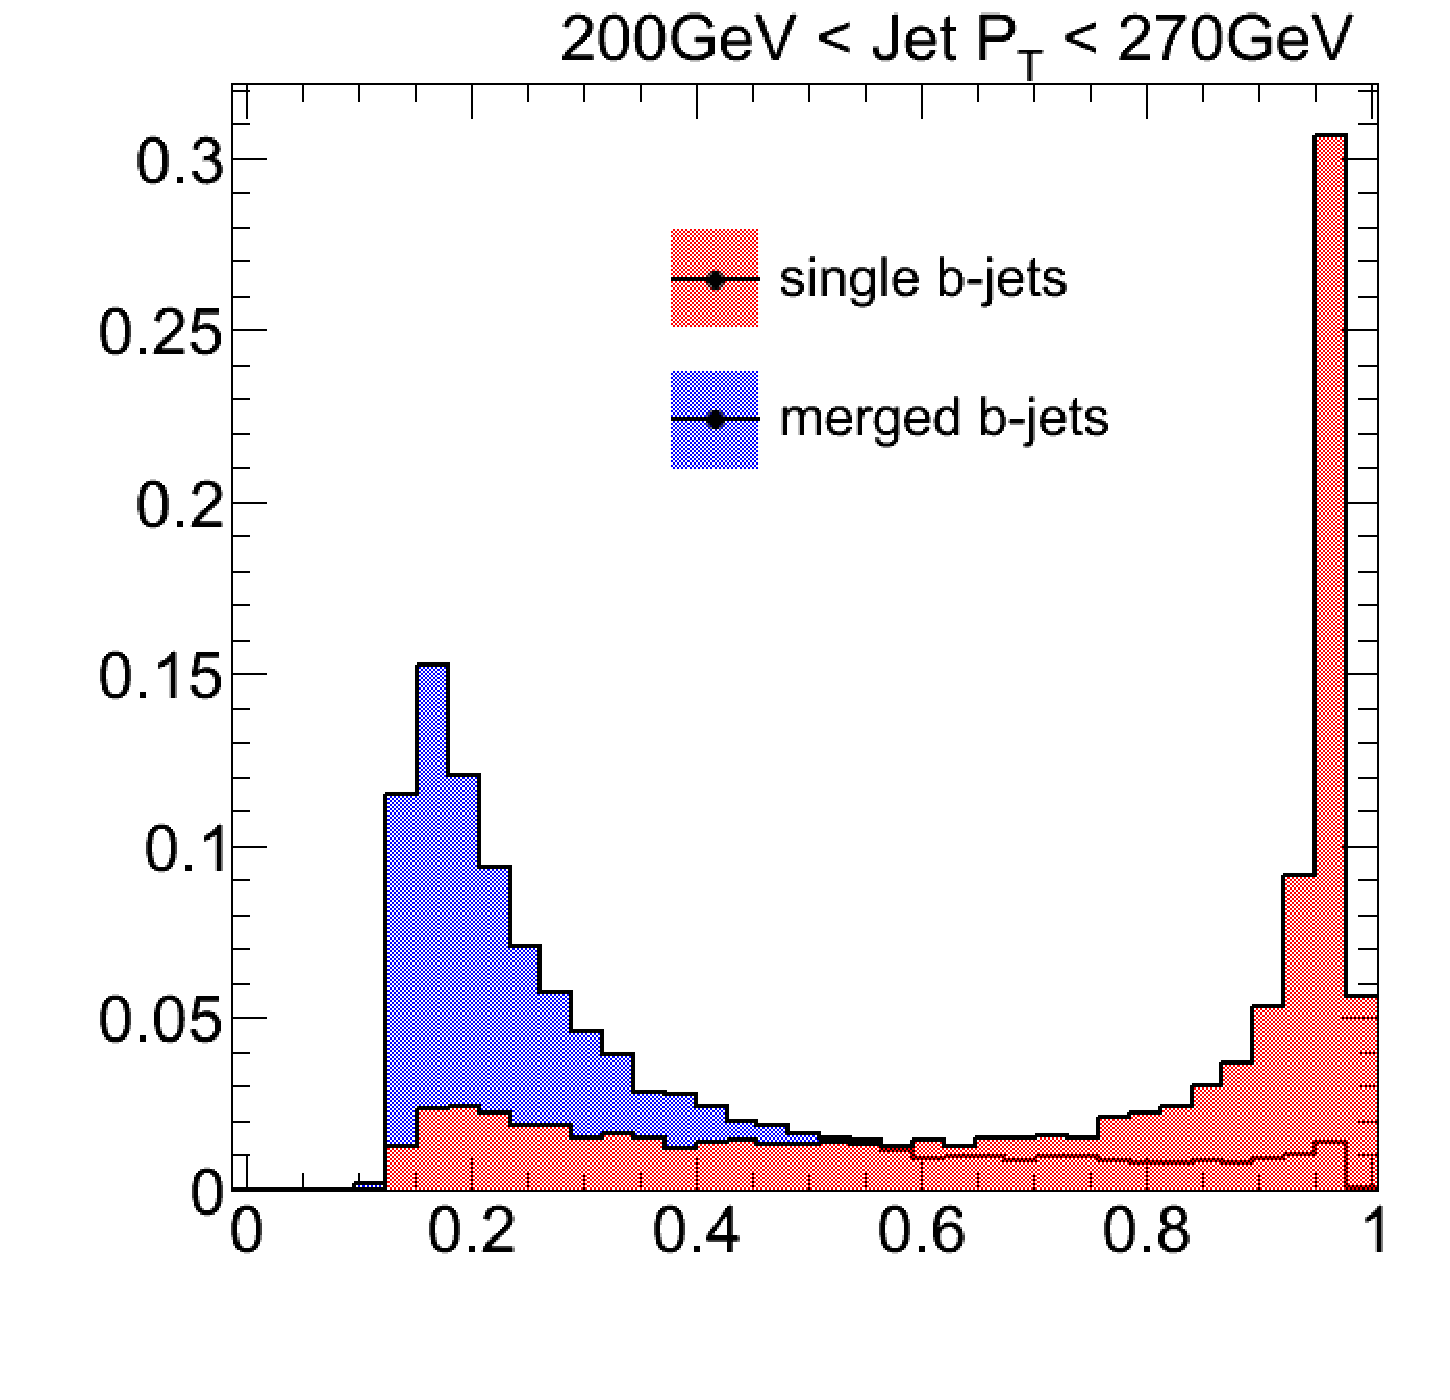
\includegraphics[width=0.32\textwidth]{FIGS/TEMPFigs/MVA_differentMethods/inclusive/NNoutput200_MLP.pdf}
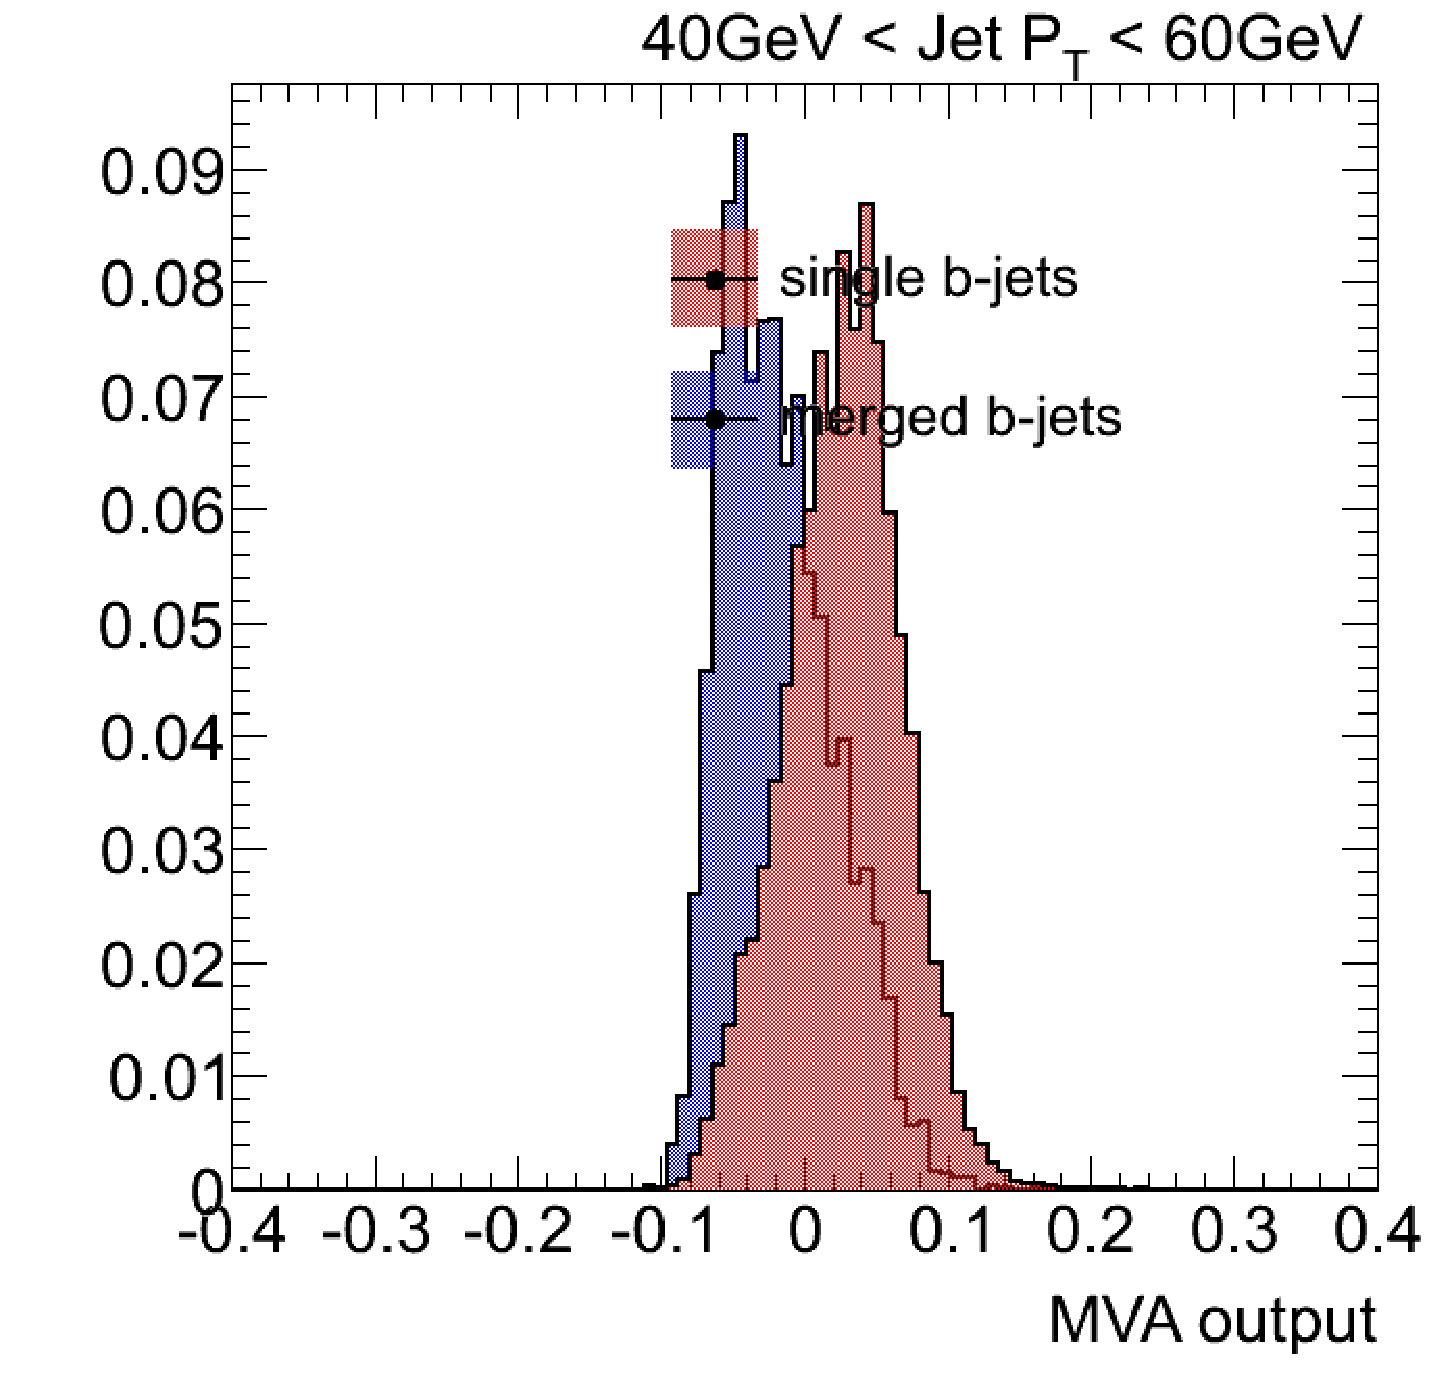
\includegraphics[width=0.32\textwidth]{FIGS/TEMPFigs/MVA_differentMethods/inclusive/NNoutput040_BDT.pdf}
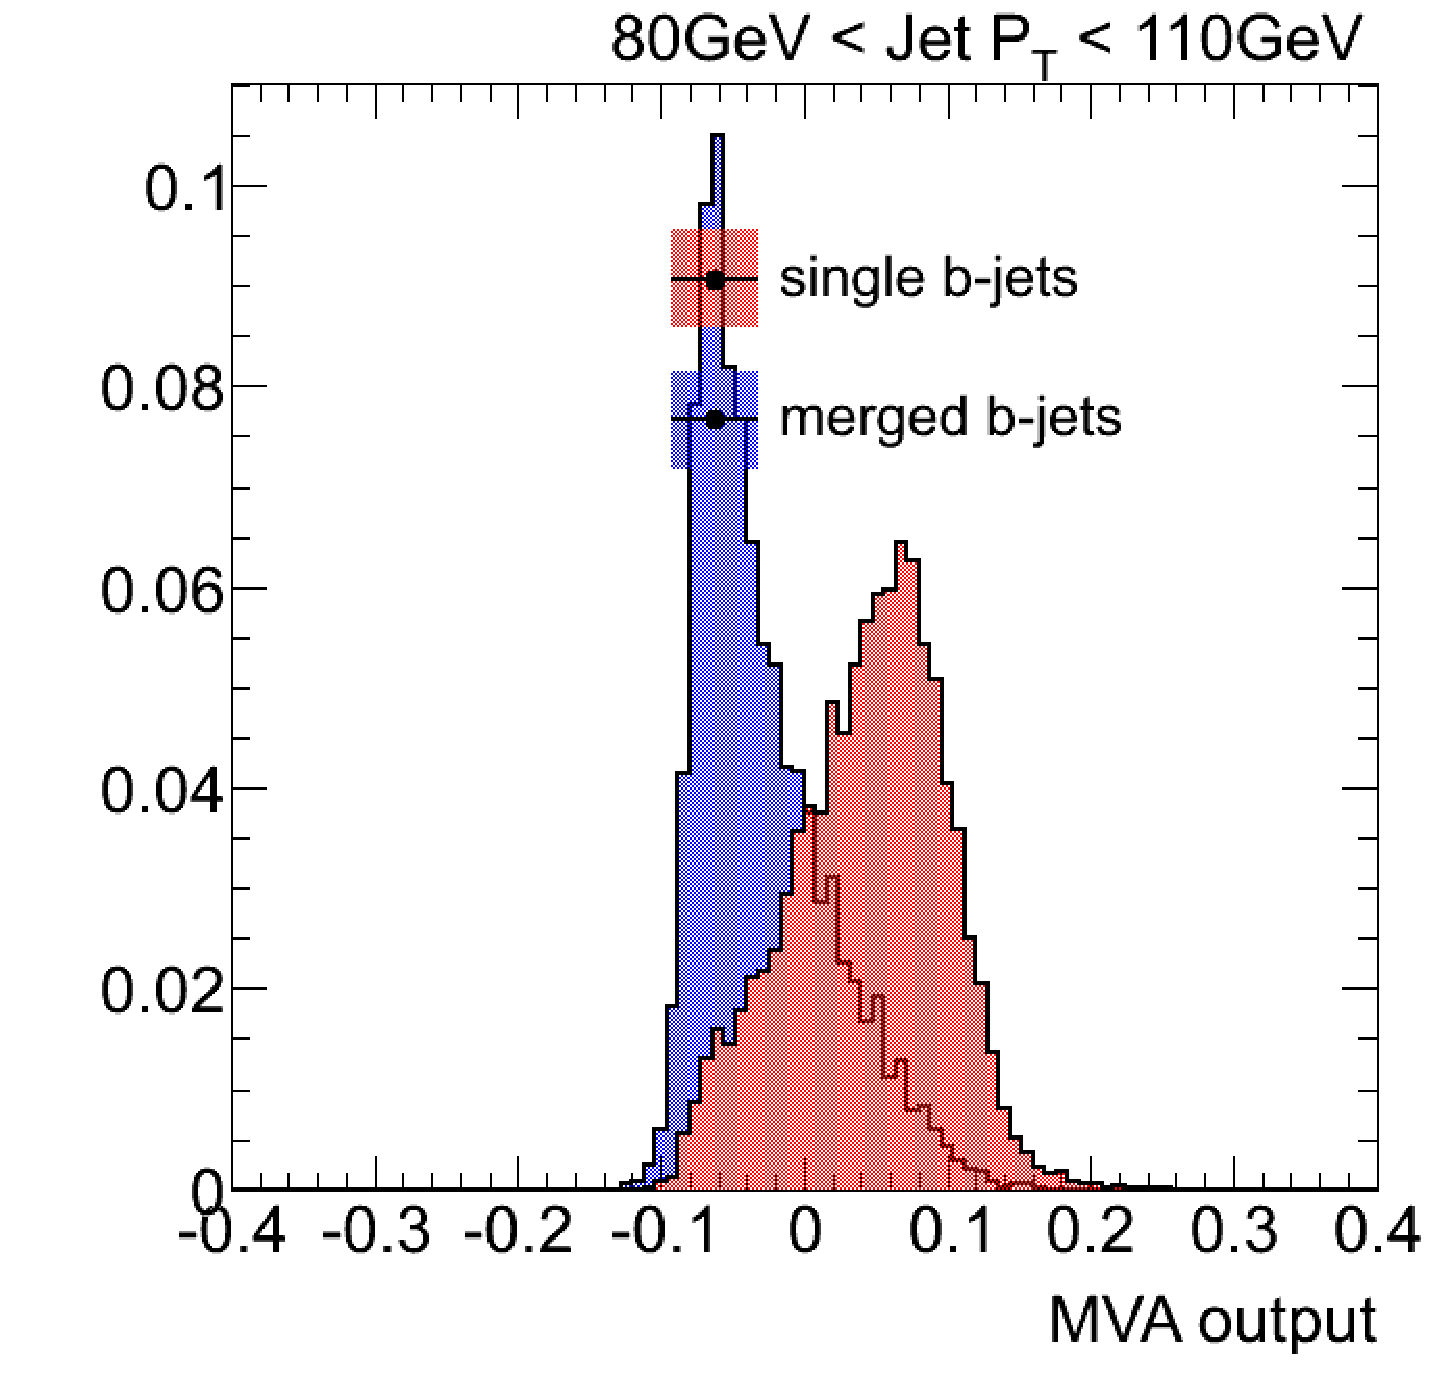
\includegraphics[width=0.32\textwidth]{FIGS/TEMPFigs/MVA_differentMethods/inclusive/NNoutput080_BDT.pdf}
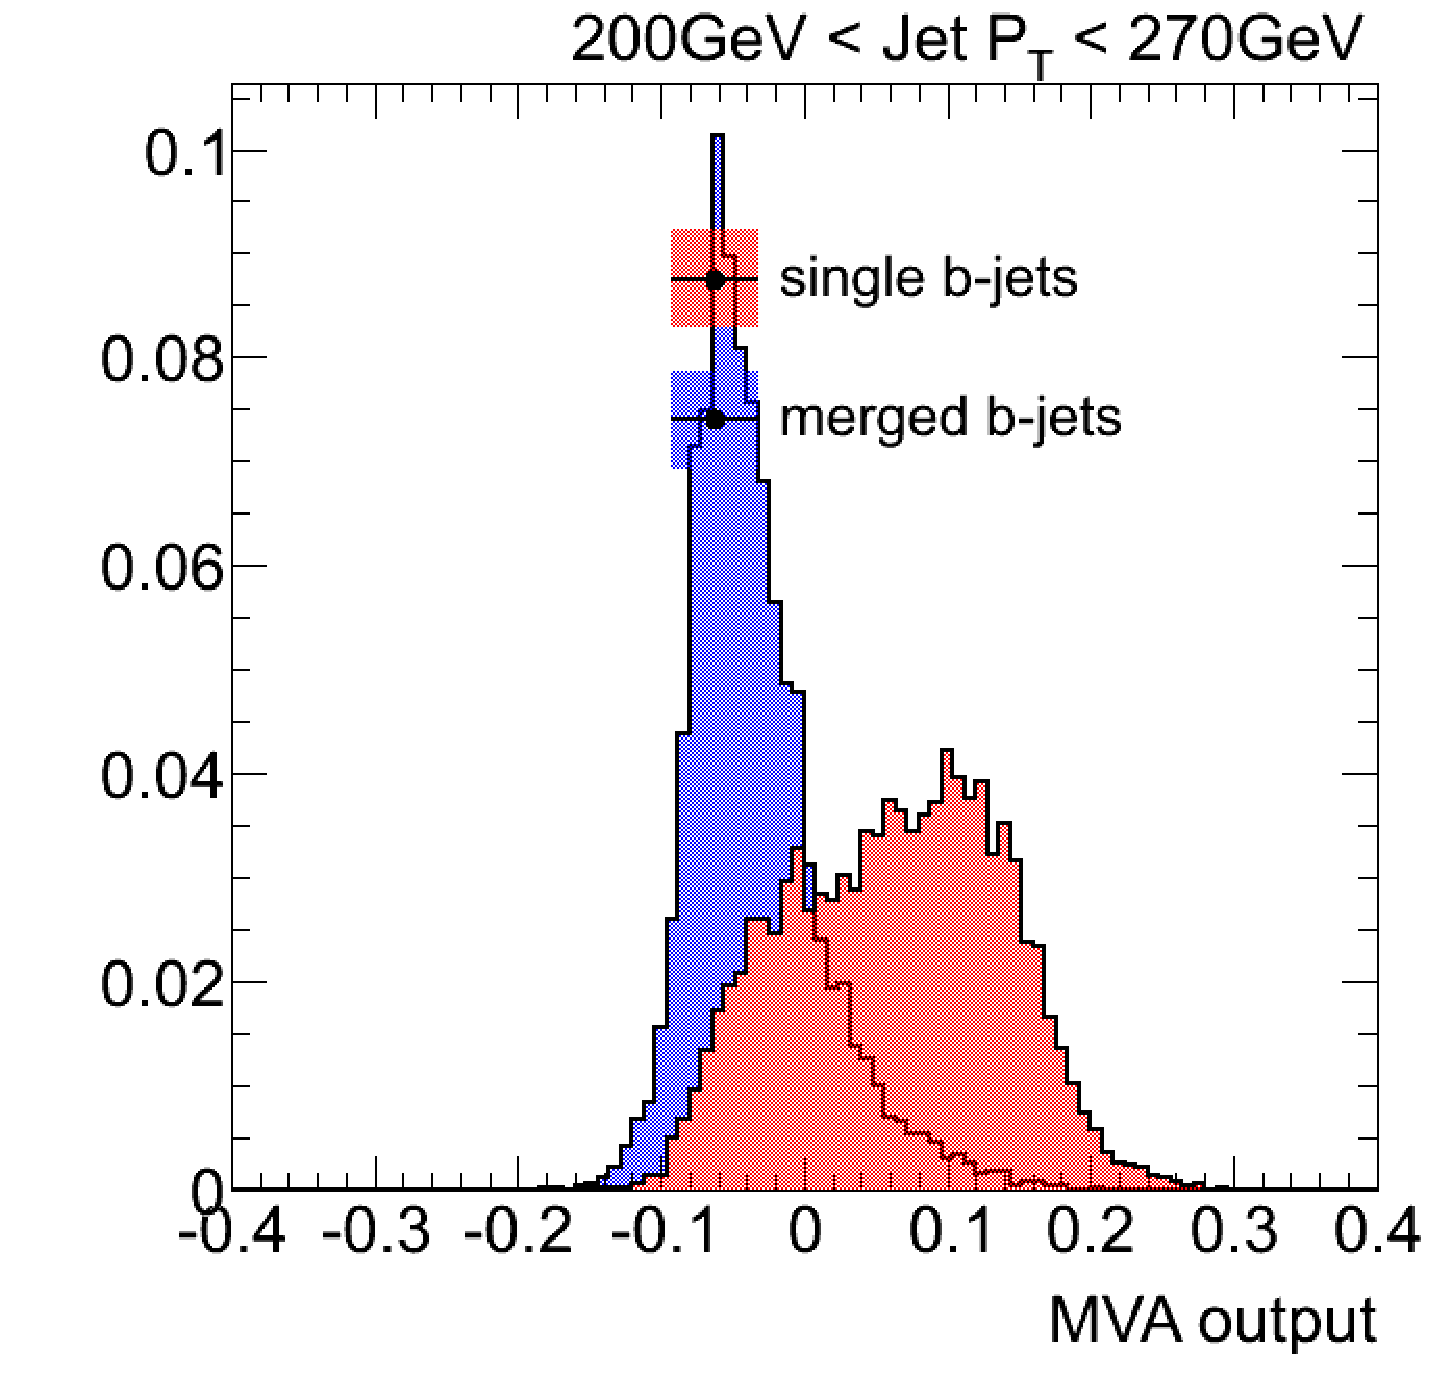
\includegraphics[width=0.32\textwidth]{FIGS/TEMPFigs/MVA_differentMethods/inclusive/NNoutput200_BDT.pdf}
\caption{Distribution of the MVA discriminant outputs, for inclusive training, in single and merged $b$-jets, for low, medium and high jet $\pt$.}
\label{fig:diffmethodsInclusive}
\end{figure}

\begin{figure}[tp]
\centering
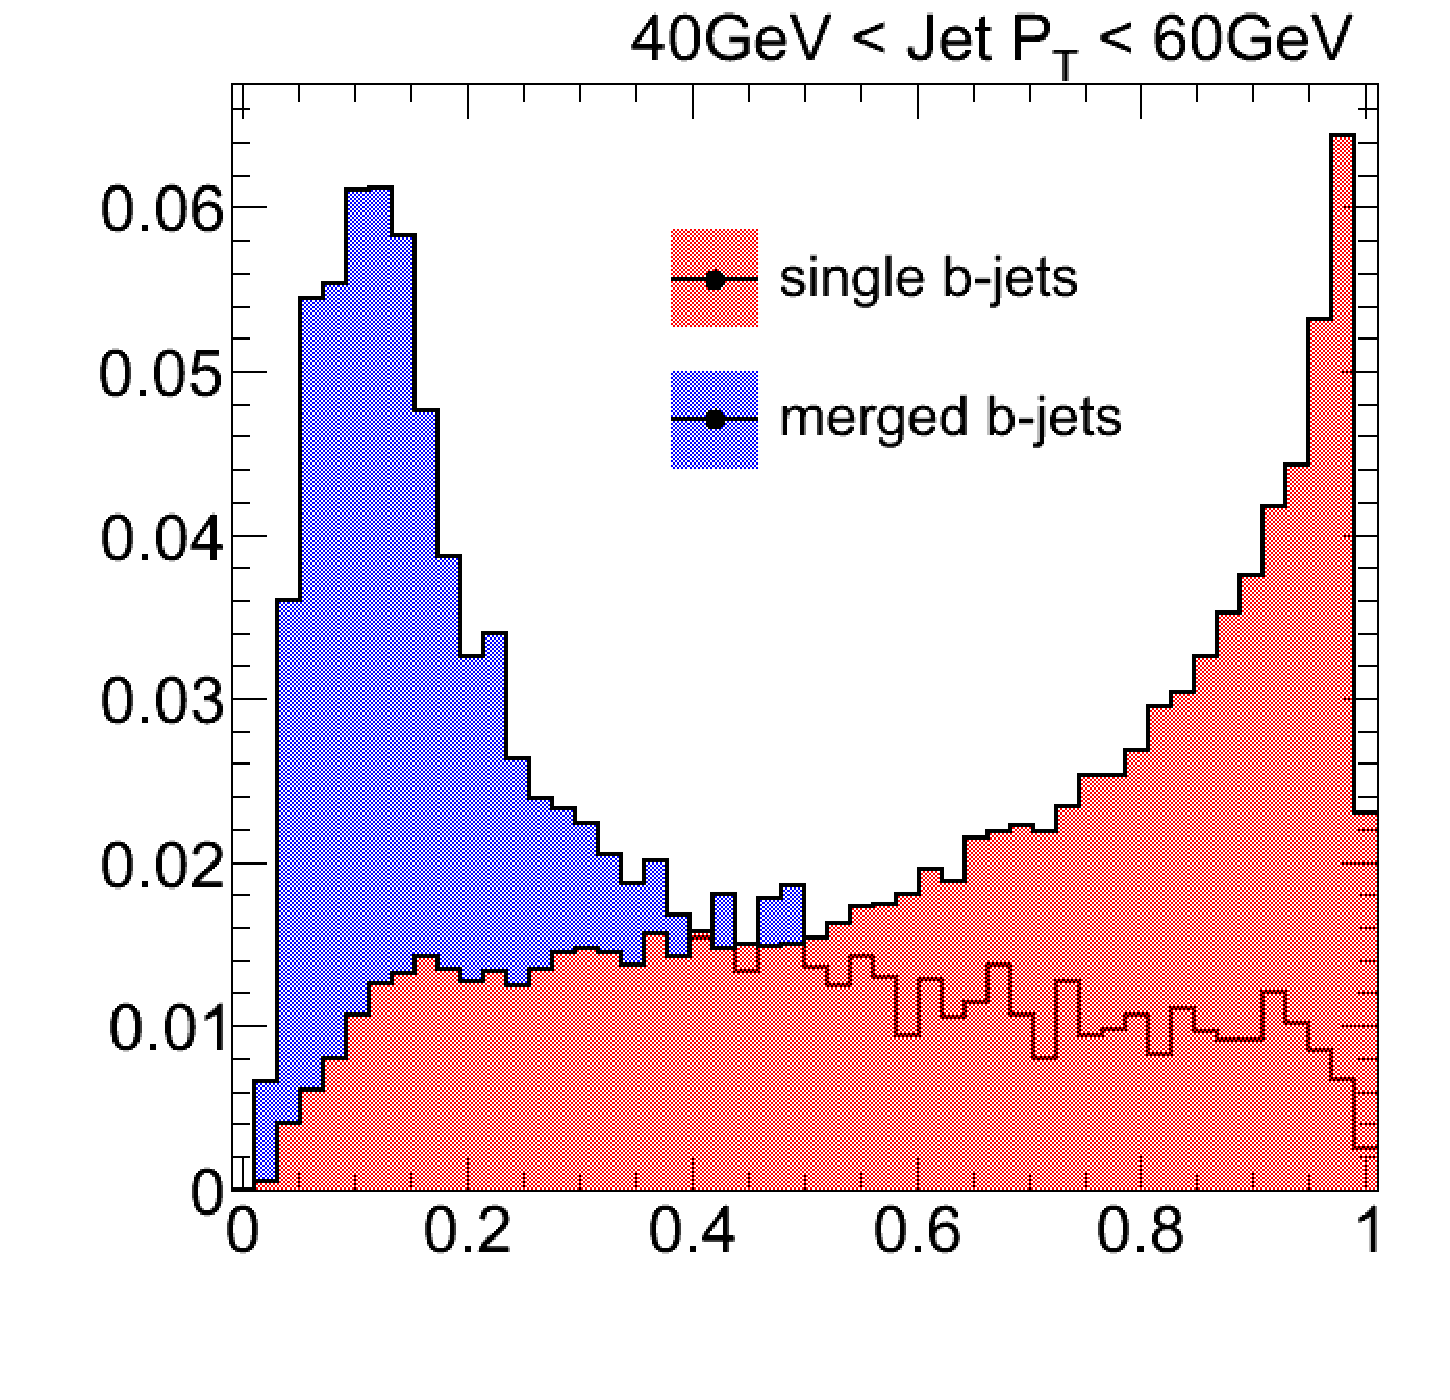
\includegraphics[width=0.32\textwidth]{FIGS/TEMPFigs/MVA_differentMethods/bins/NNoutput040_LihoodKDE.pdf}
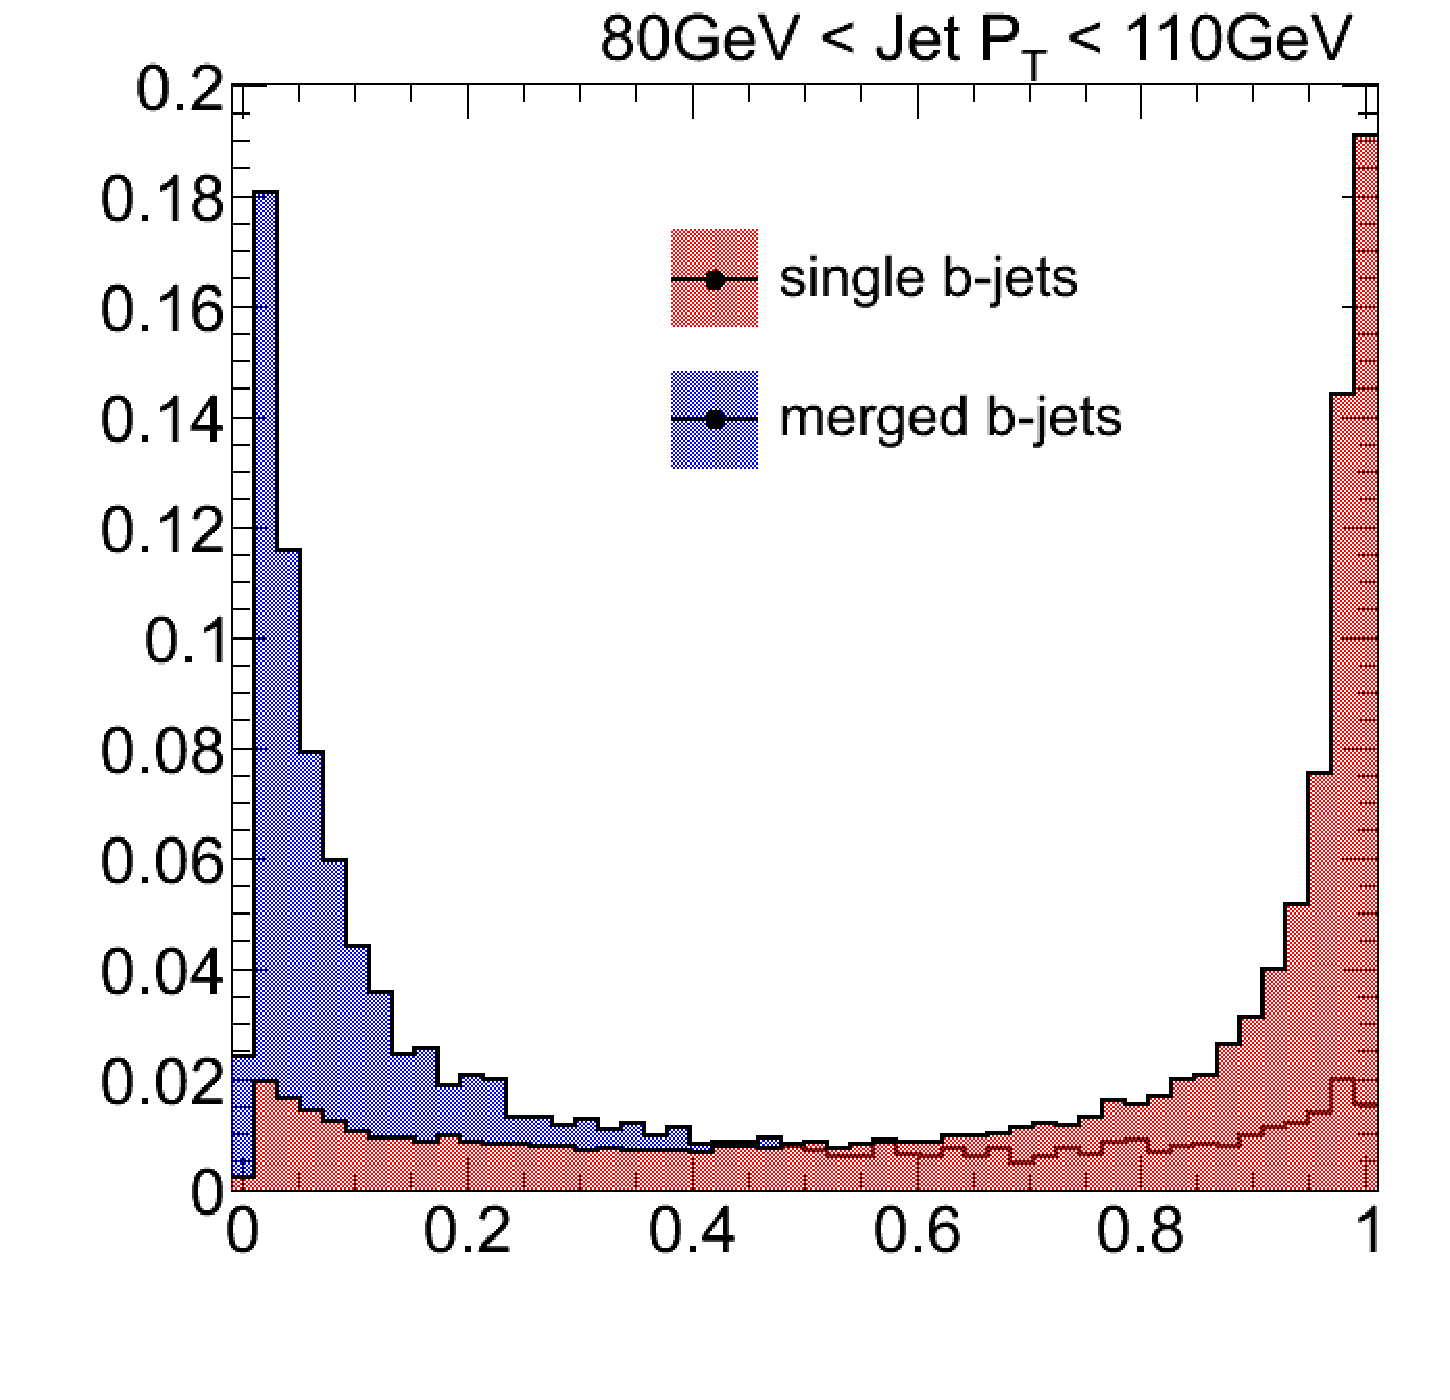
\includegraphics[width=0.32\textwidth]{FIGS/TEMPFigs/MVA_differentMethods/bins/NNoutput080_LihoodKDE.pdf}
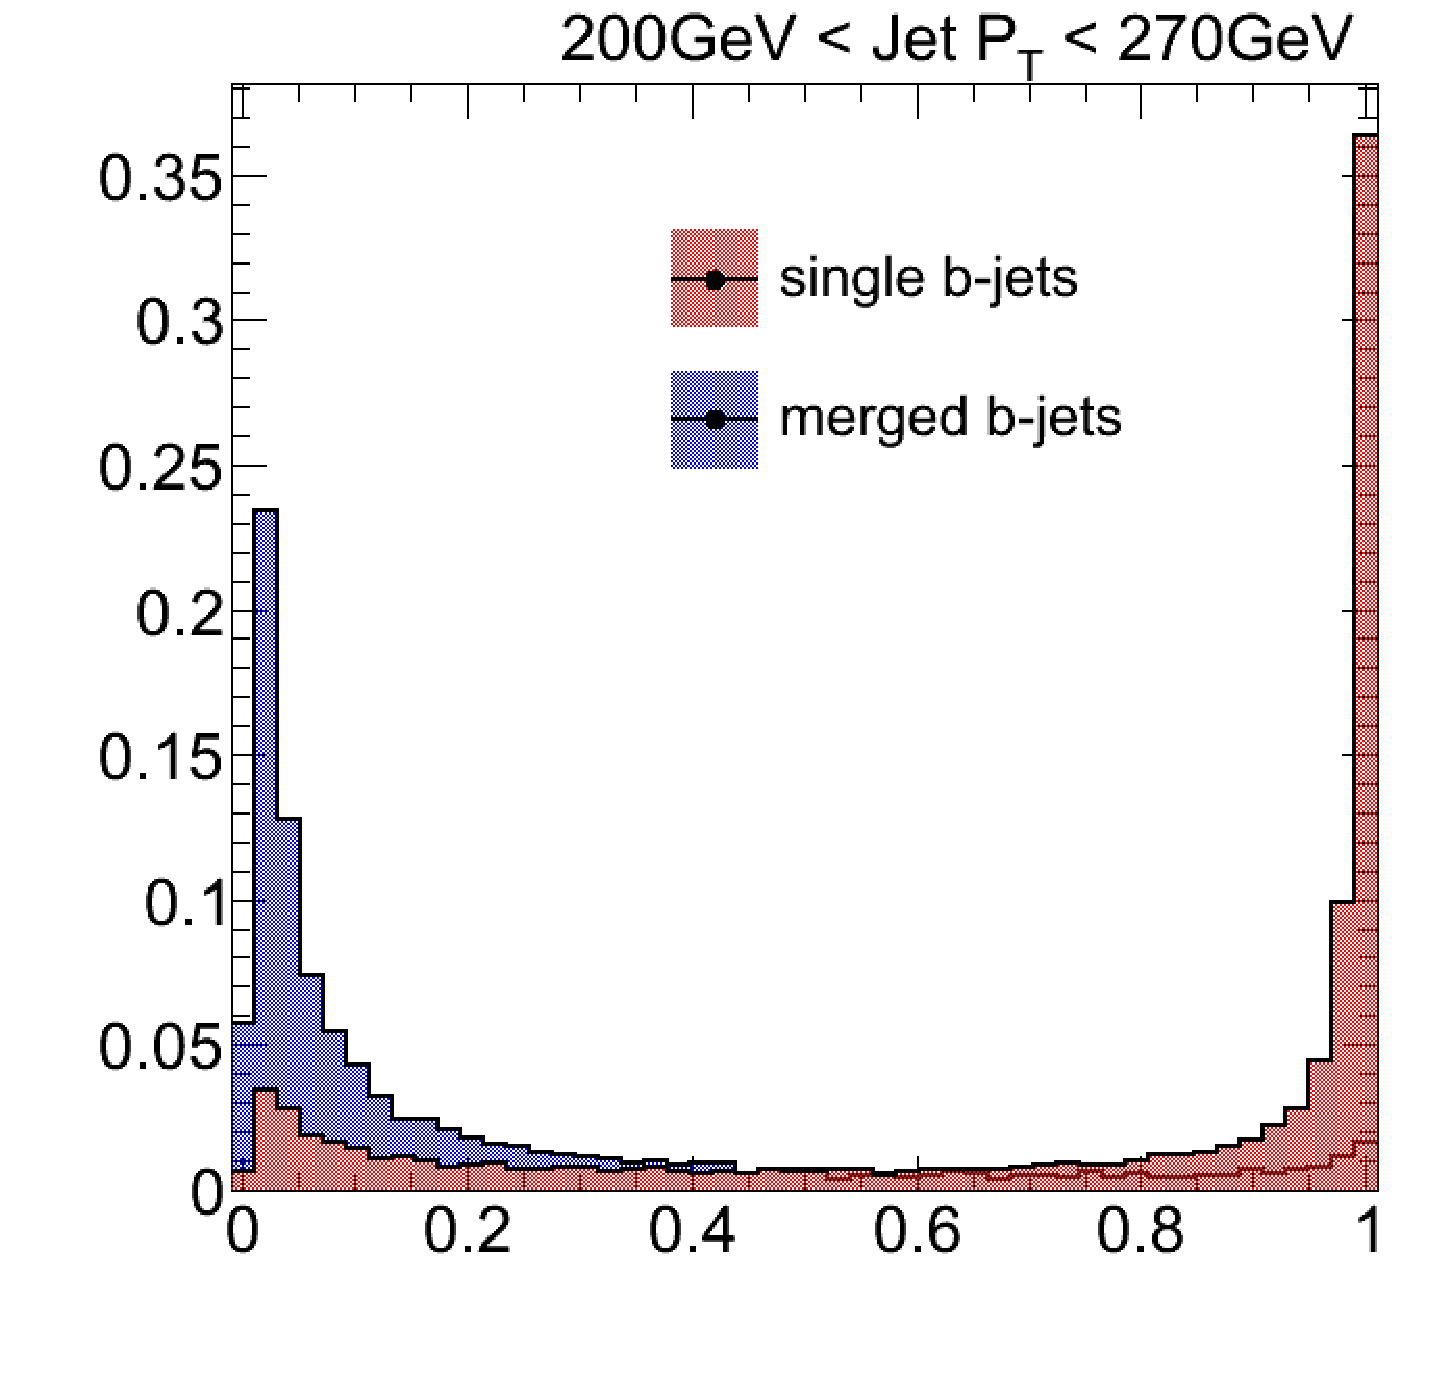
\includegraphics[width=0.32\textwidth]{FIGS/TEMPFigs/MVA_differentMethods/bins/NNoutput200_LihoodKDE.pdf}
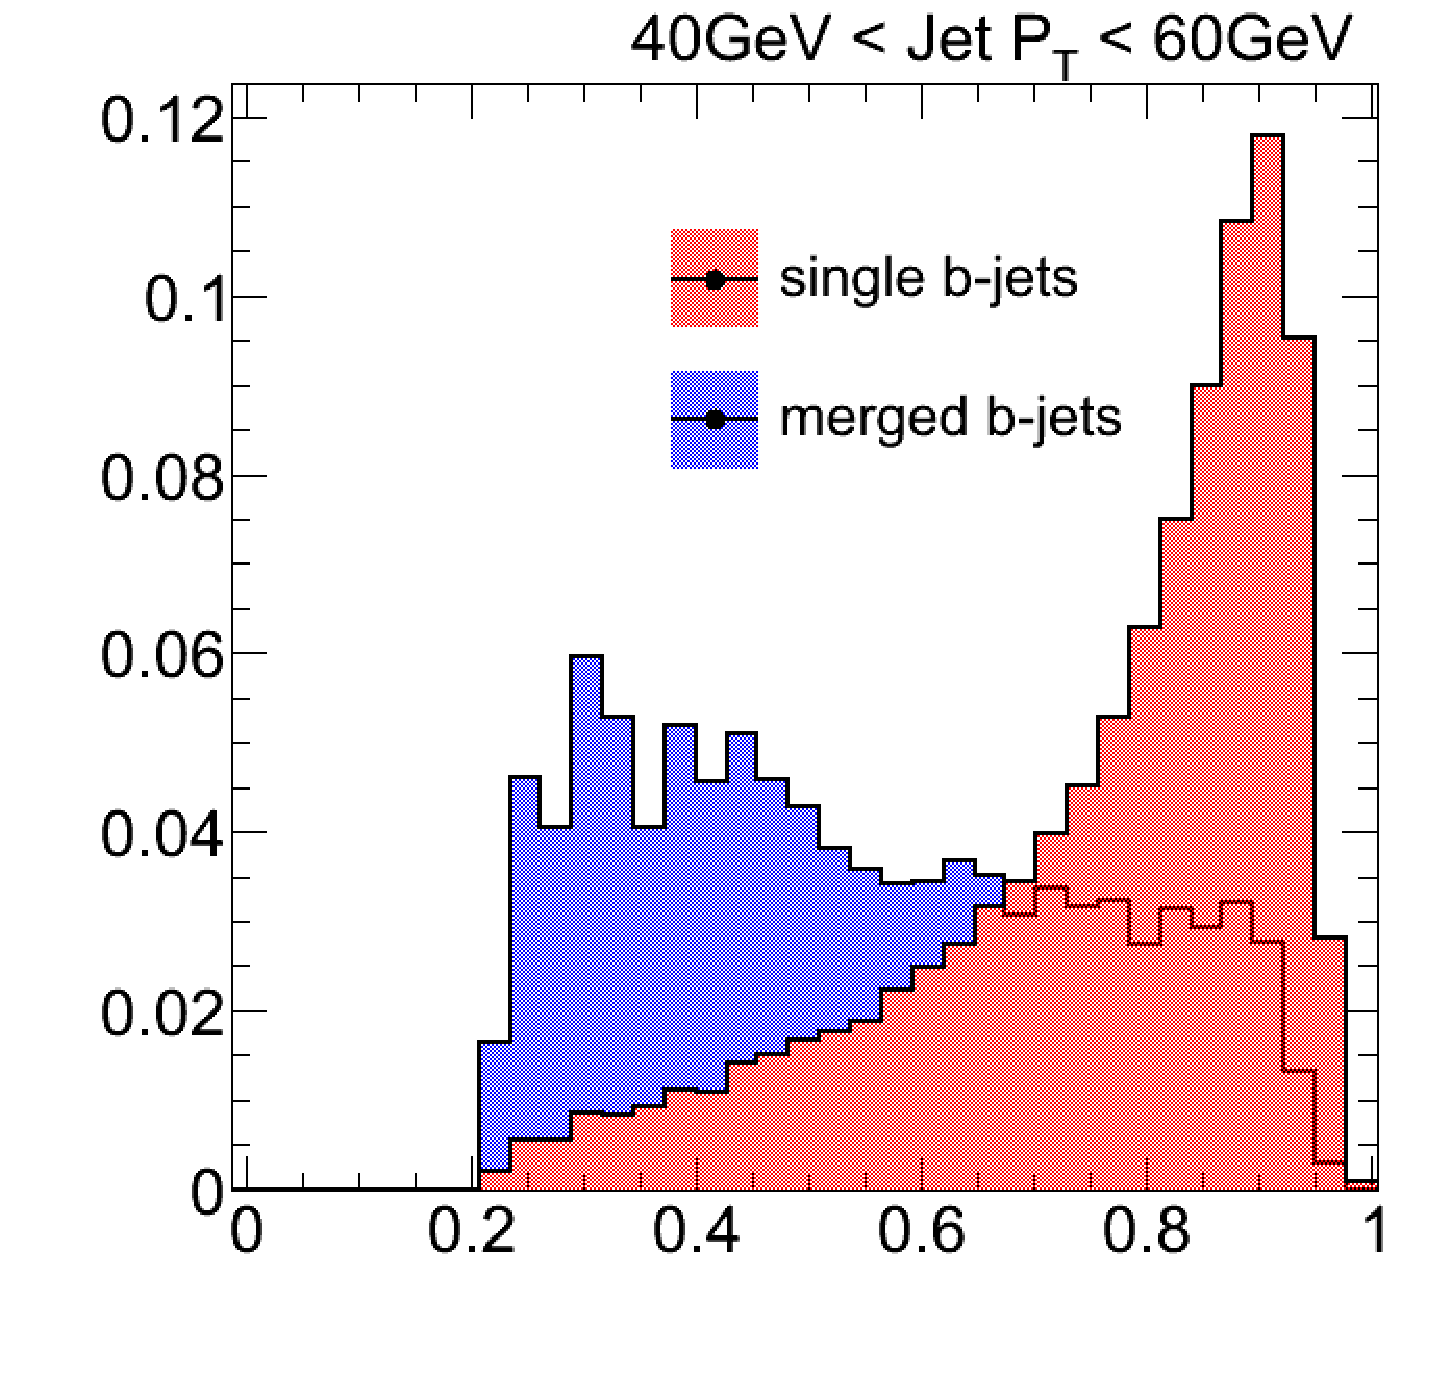
\includegraphics[width=0.32\textwidth]{FIGS/TEMPFigs/MVA_differentMethods/bins/NNoutput040_MLP.pdf}
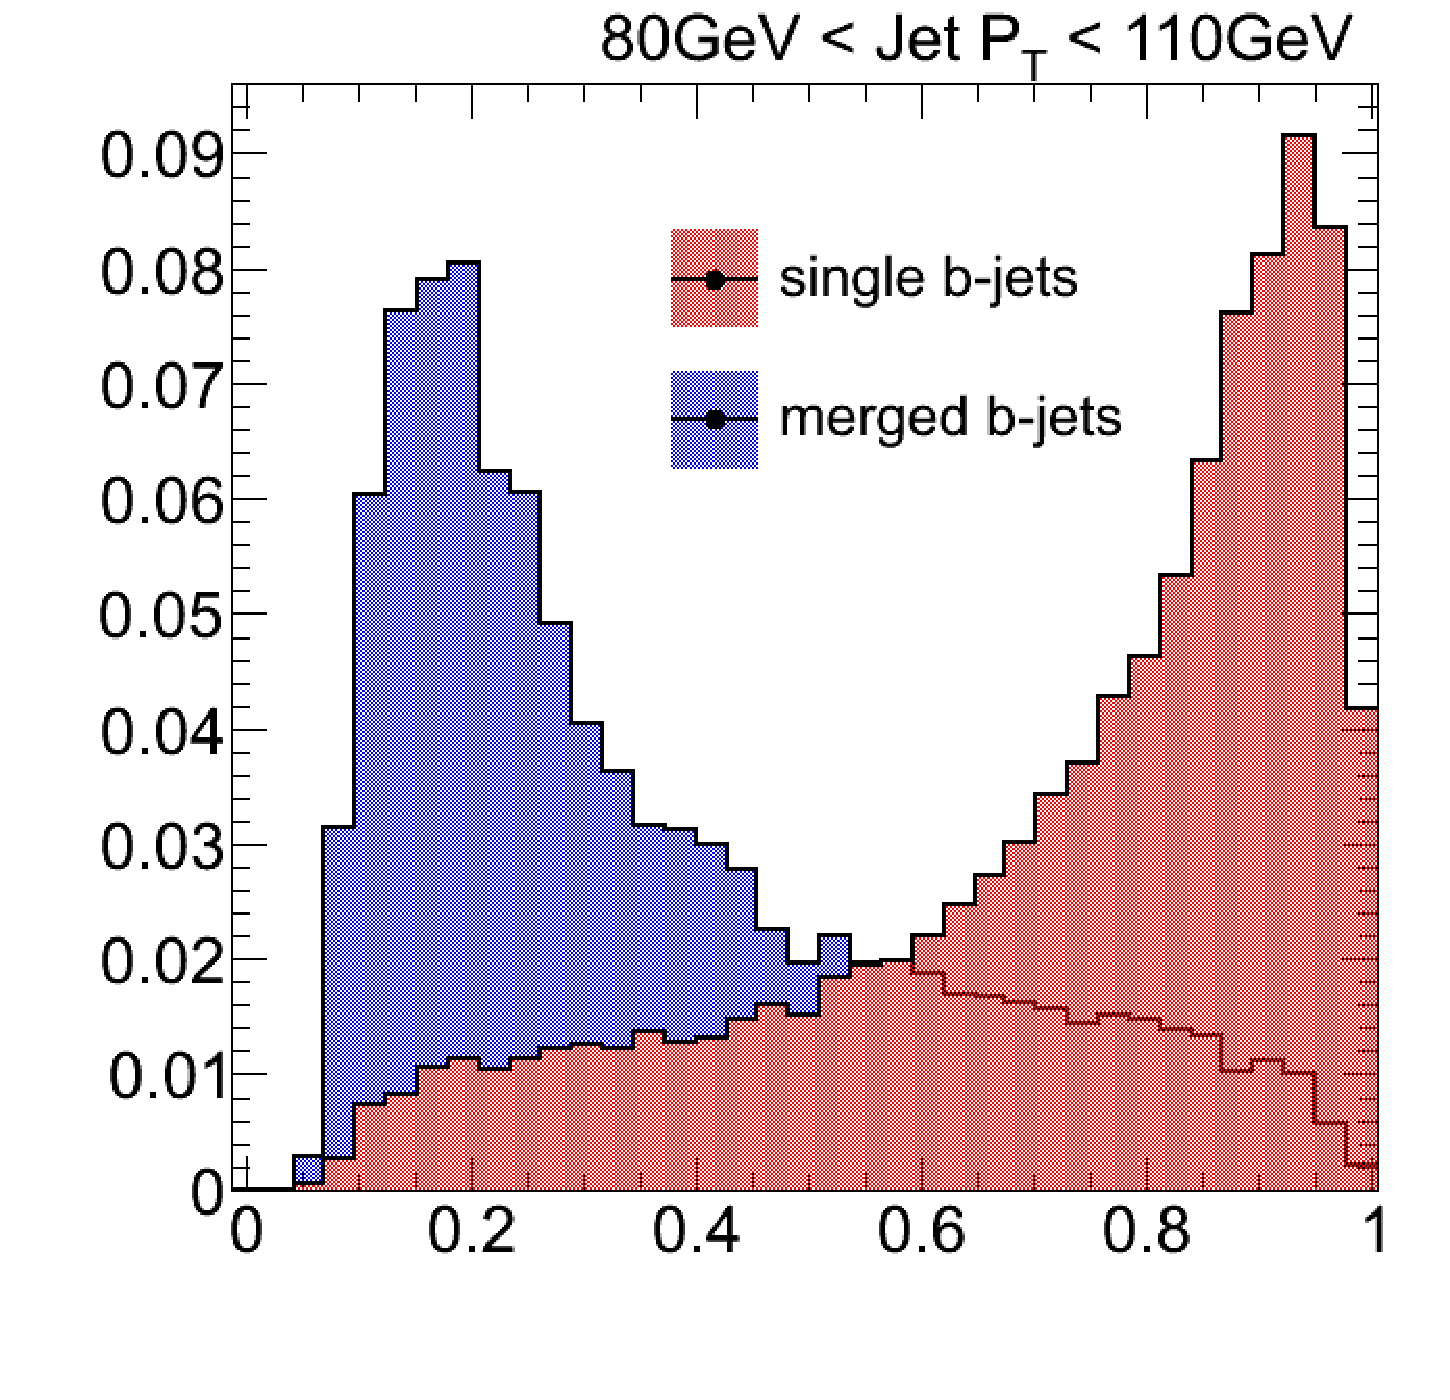
\includegraphics[width=0.32\textwidth]{FIGS/TEMPFigs/MVA_differentMethods/bins/NNoutput080_MLP.pdf}
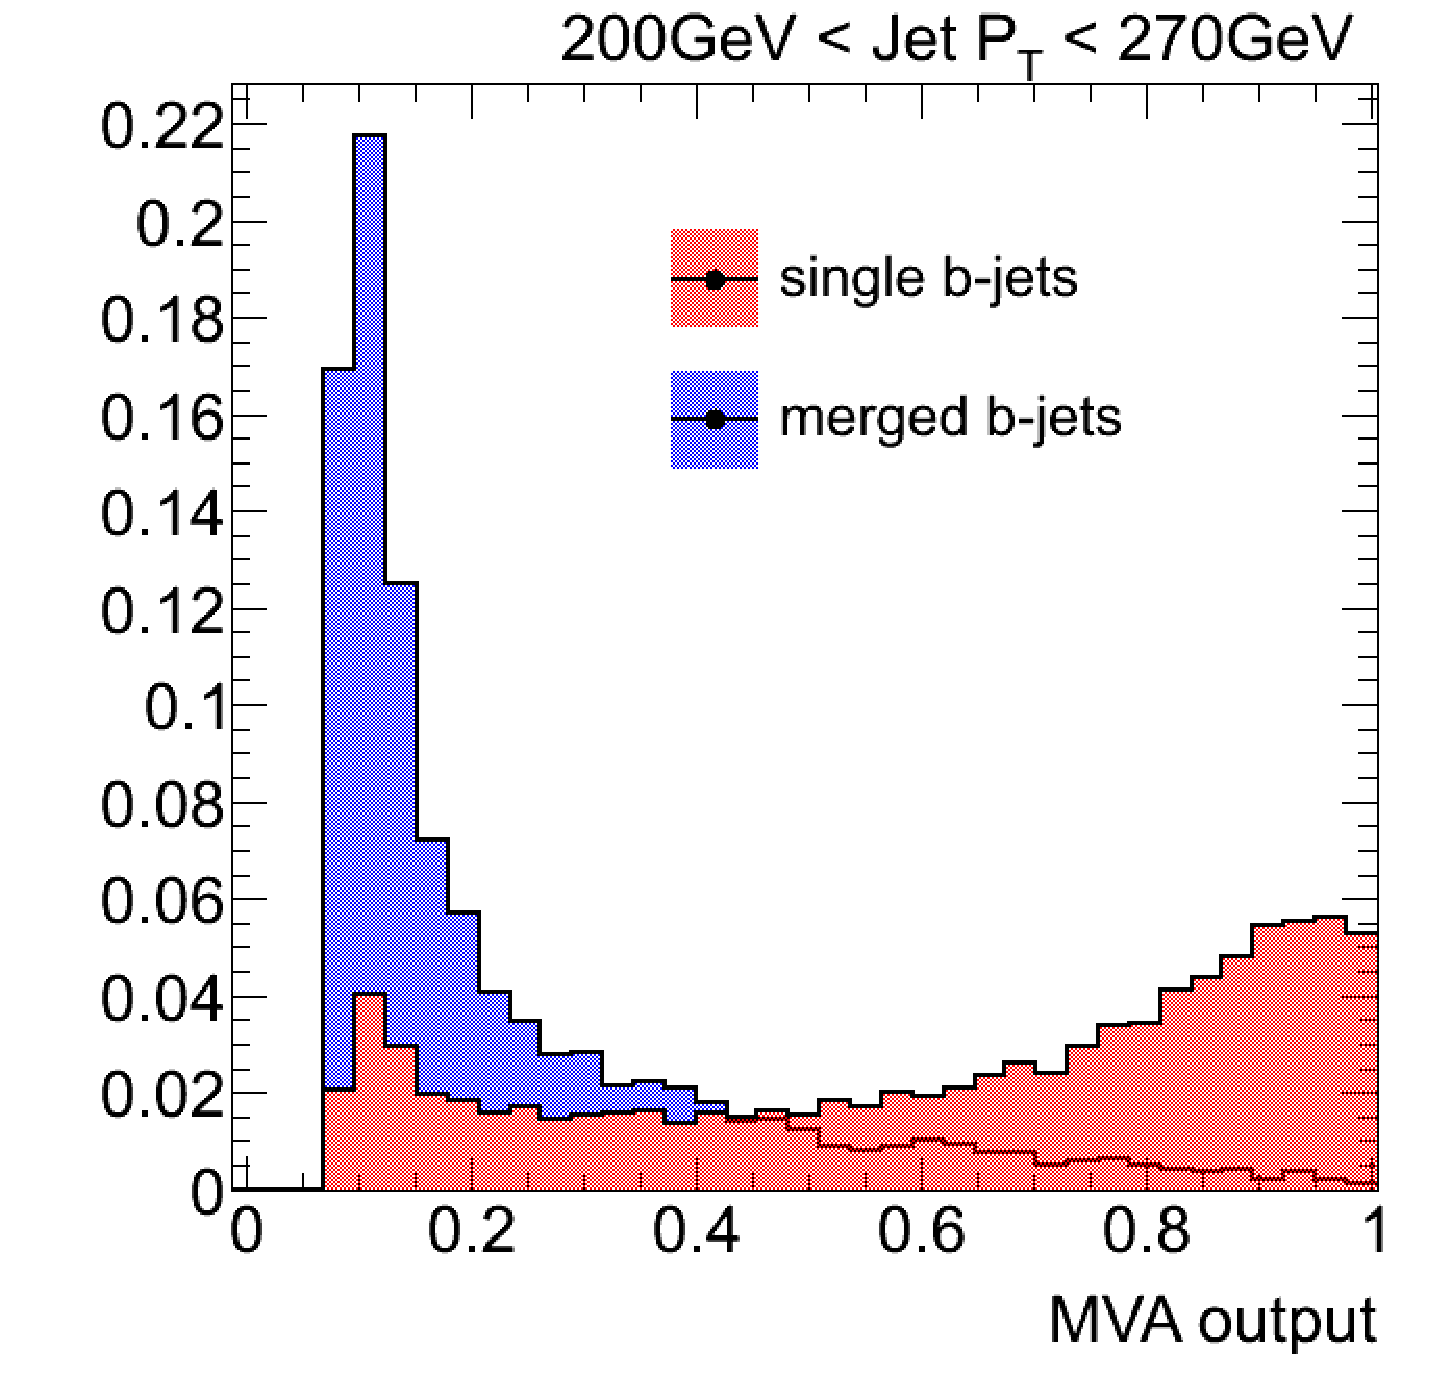
\includegraphics[width=0.32\textwidth]{FIGS/TEMPFigs/MVA_differentMethods/bins/NNoutput200_MLP.pdf}
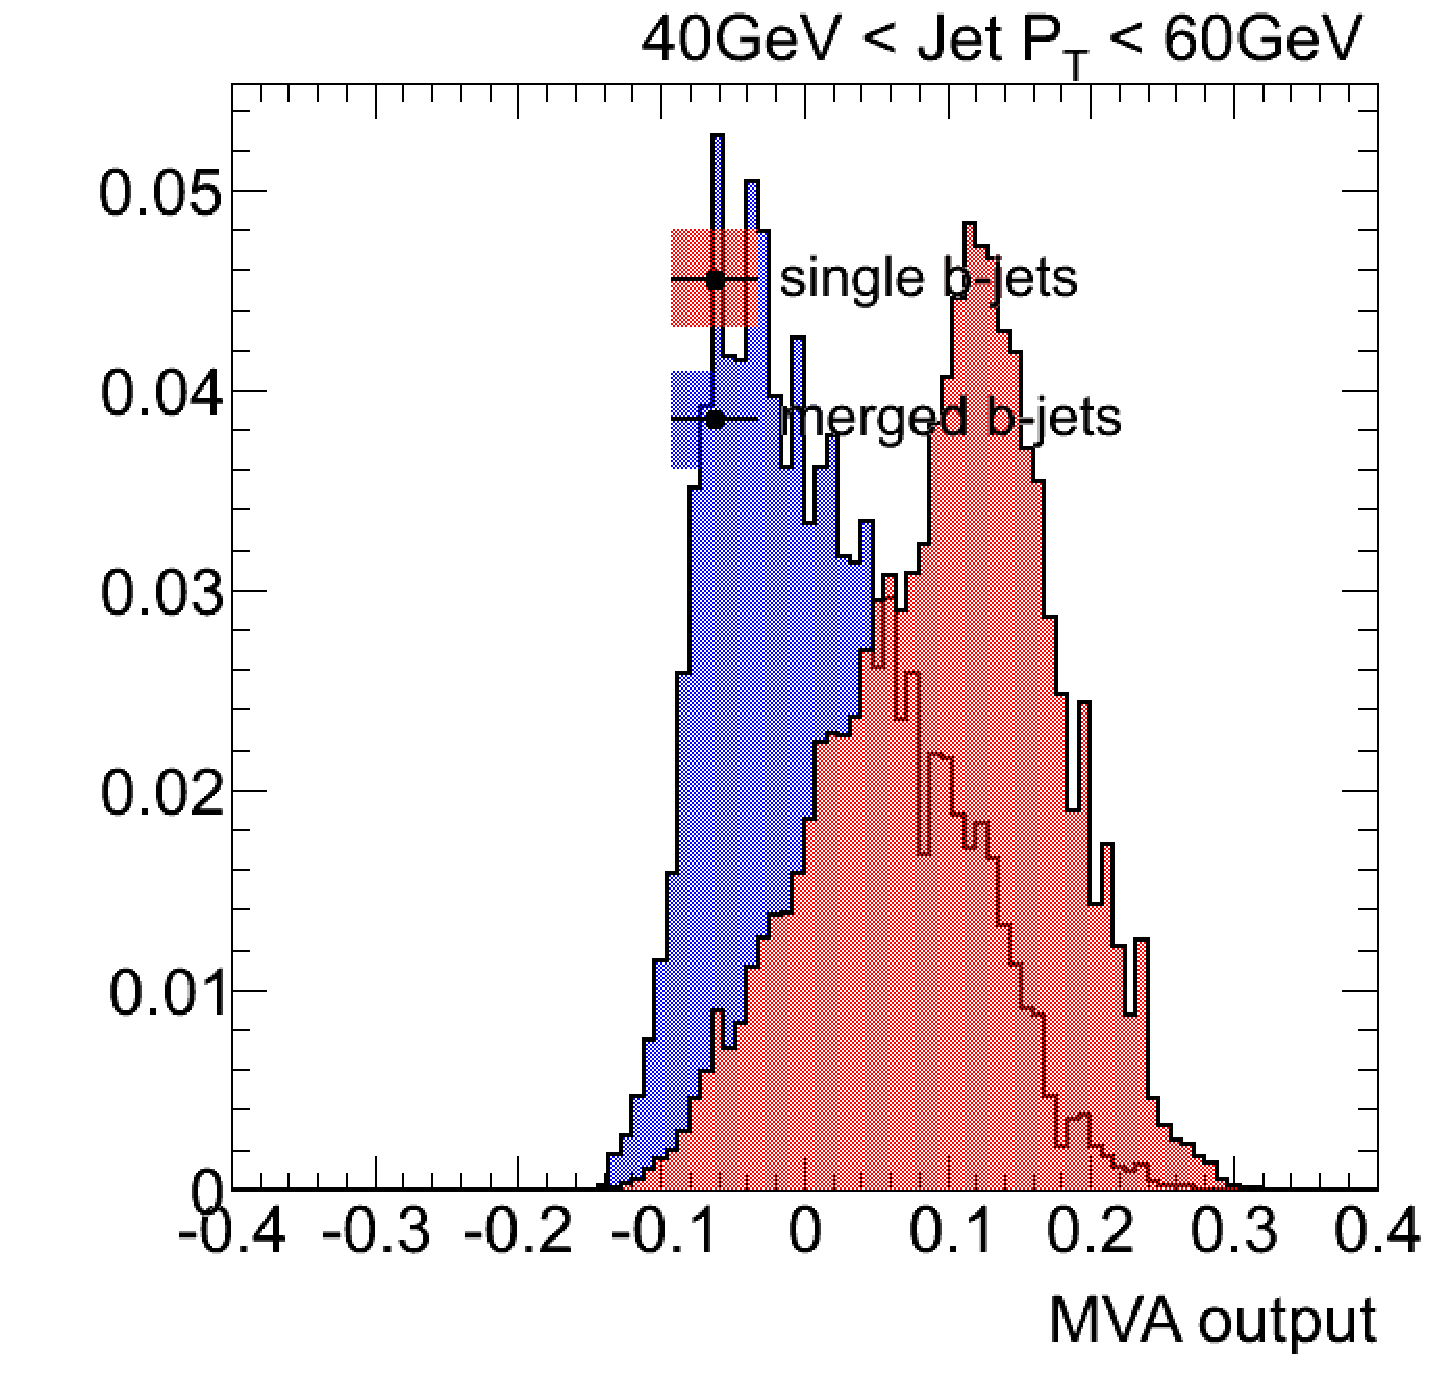
\includegraphics[width=0.32\textwidth]{FIGS/TEMPFigs/MVA_differentMethods/bins/NNoutput040_BDT.pdf}
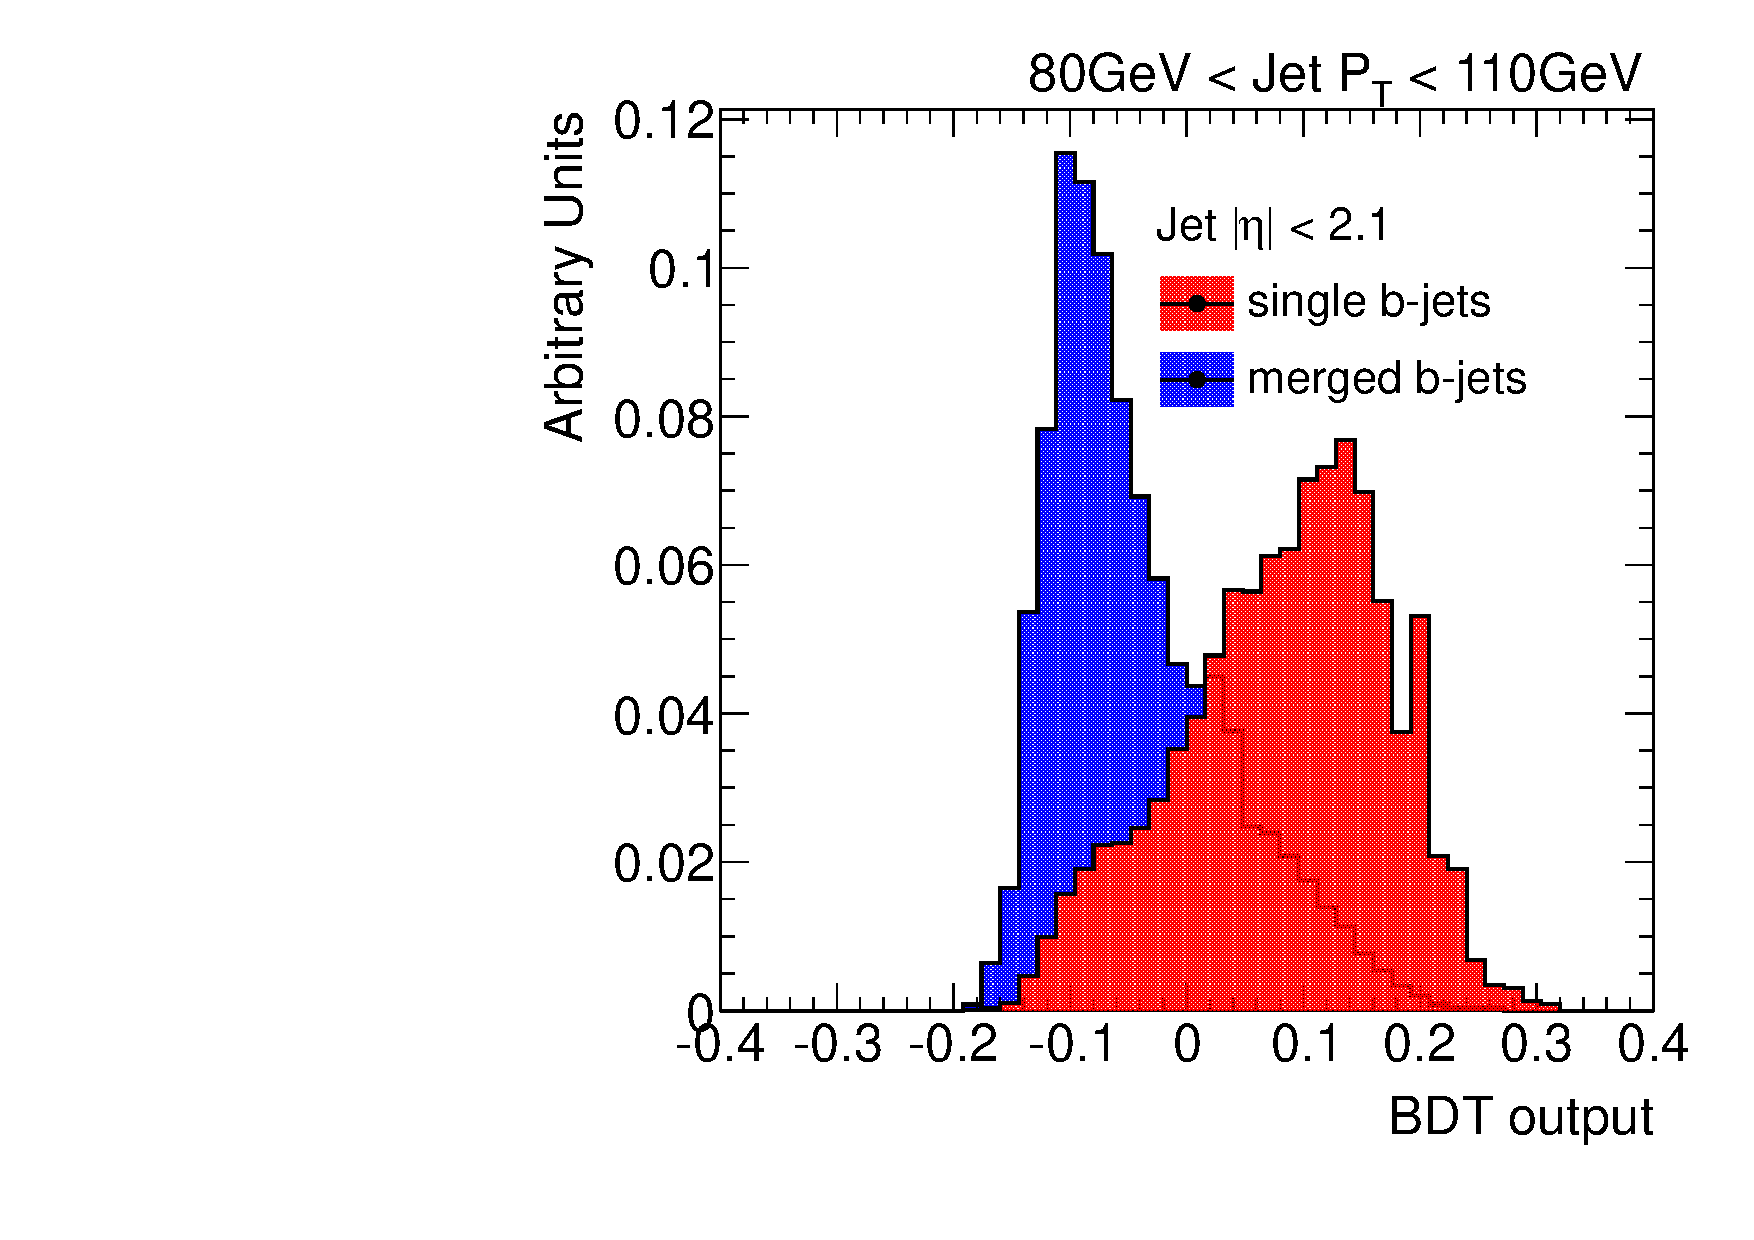
\includegraphics[width=0.32\textwidth]{FIGS/TEMPFigs/MVA_differentMethods/bins/NNoutput080_BDT.pdf}
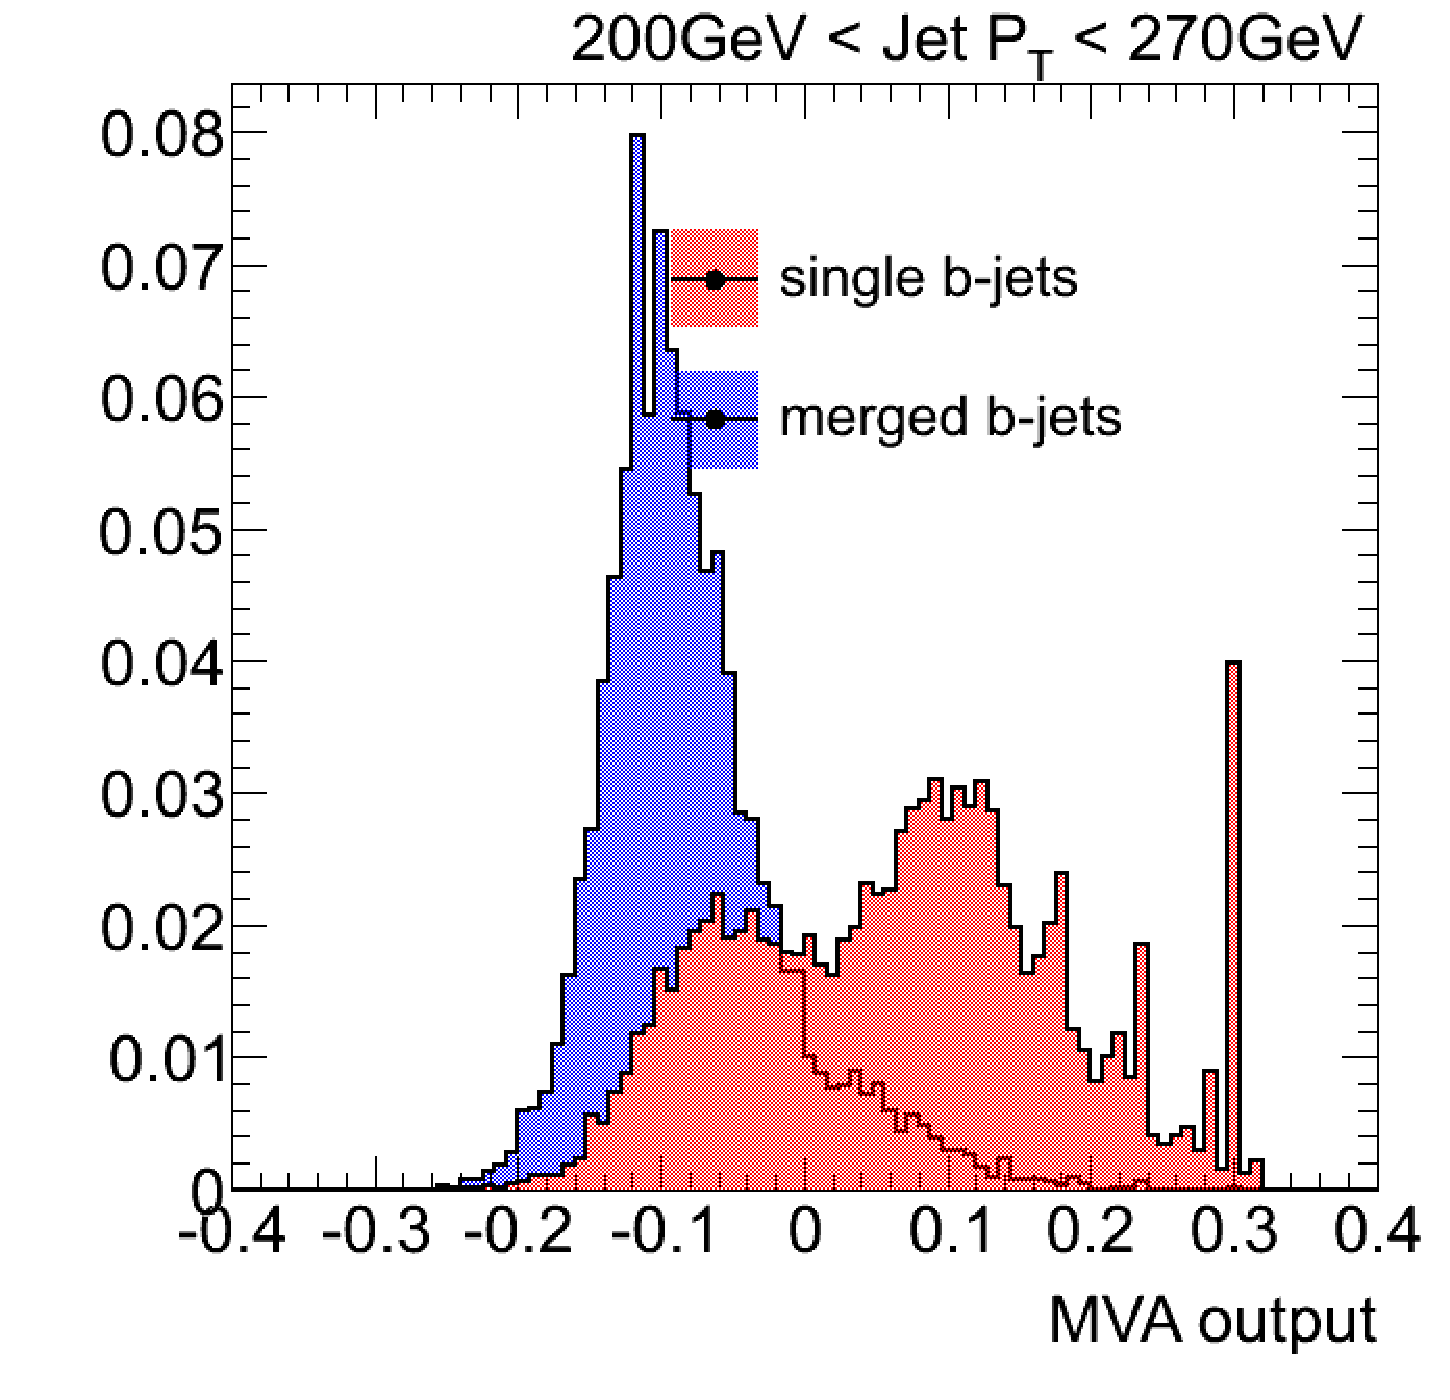
\includegraphics[width=0.32\textwidth]{FIGS/TEMPFigs/MVA_differentMethods/bins/NNoutput200_BDT.pdf}
\caption{Distribution of the MVA discriminant outputs, for training in bins of jet $\pt$, in single and merged $b$-jets, for low, medium and high jet $\pt$.}
\label{fig:diffmethodsBins}
\end{figure}

\begin{figure}[tp]
\centering
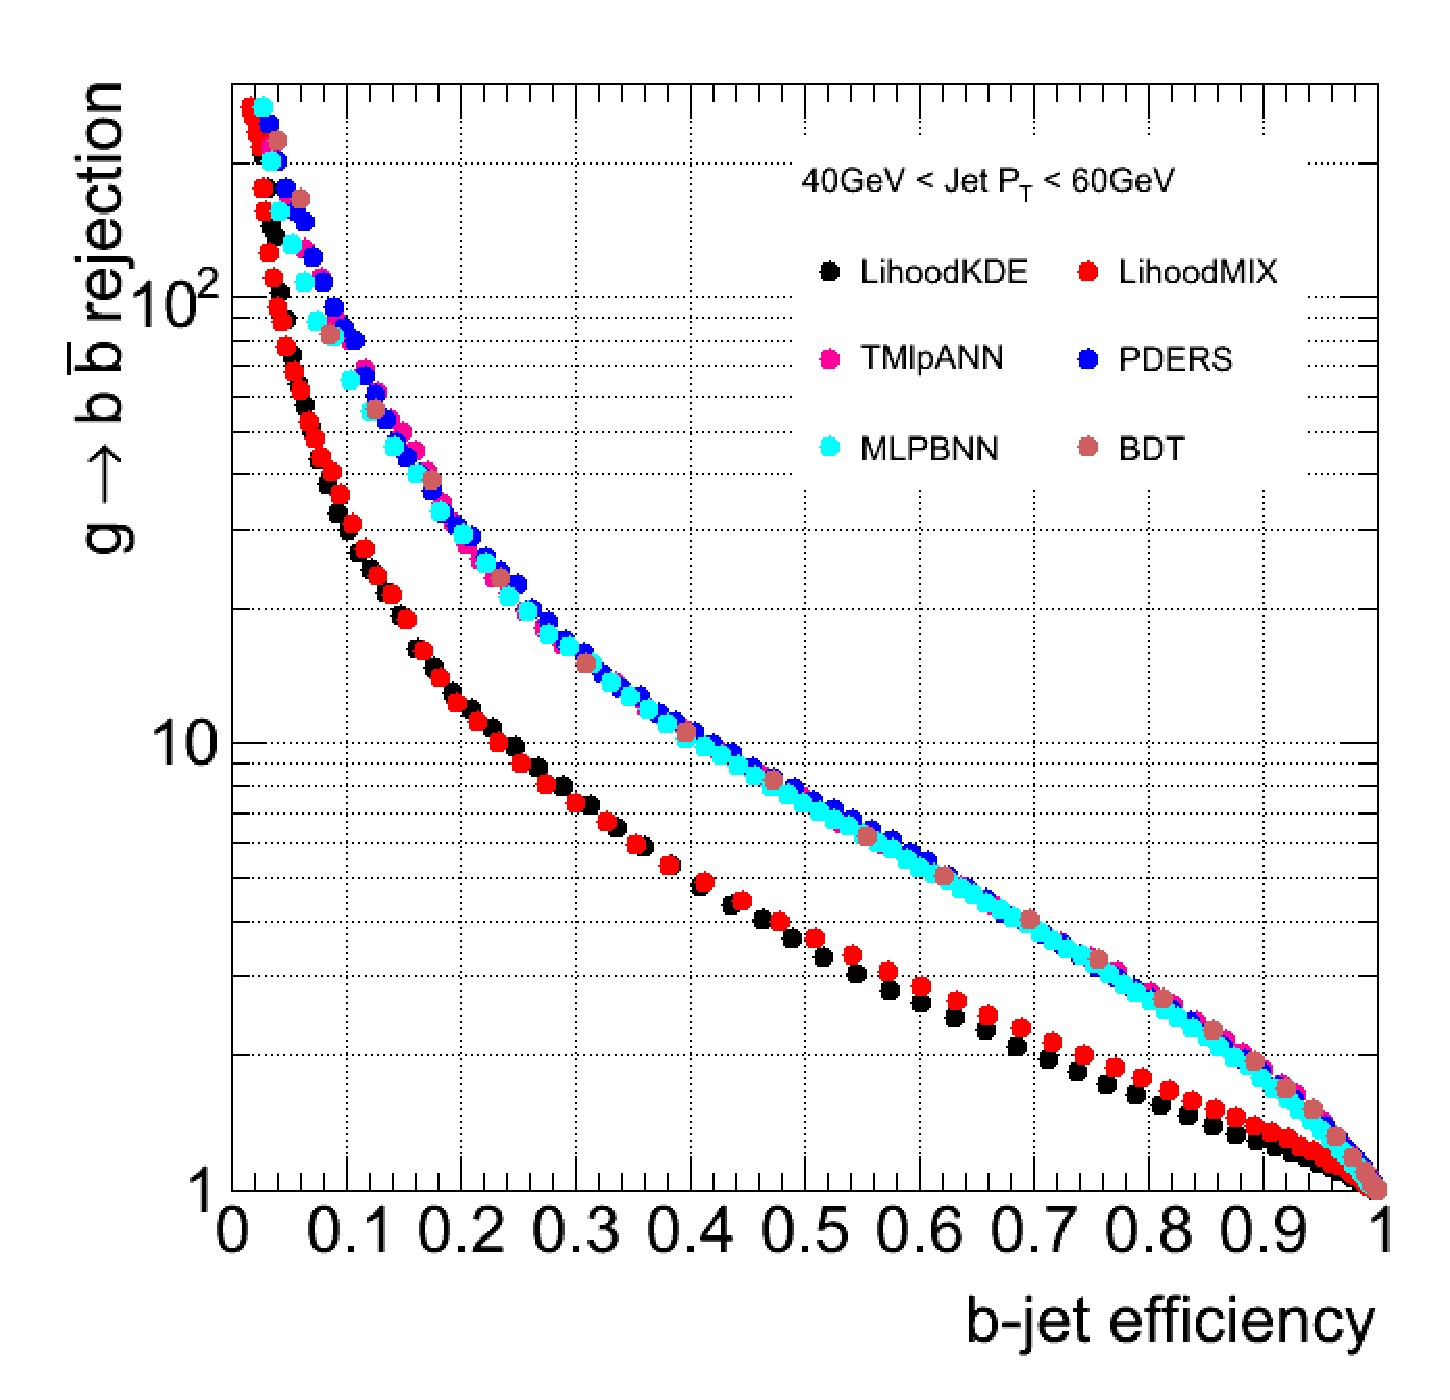
\includegraphics[width=0.49\textwidth]{FIGS/TEMPFigs/MVA_differentMethods/inclusive/MVAs_RejvsEff40.pdf}
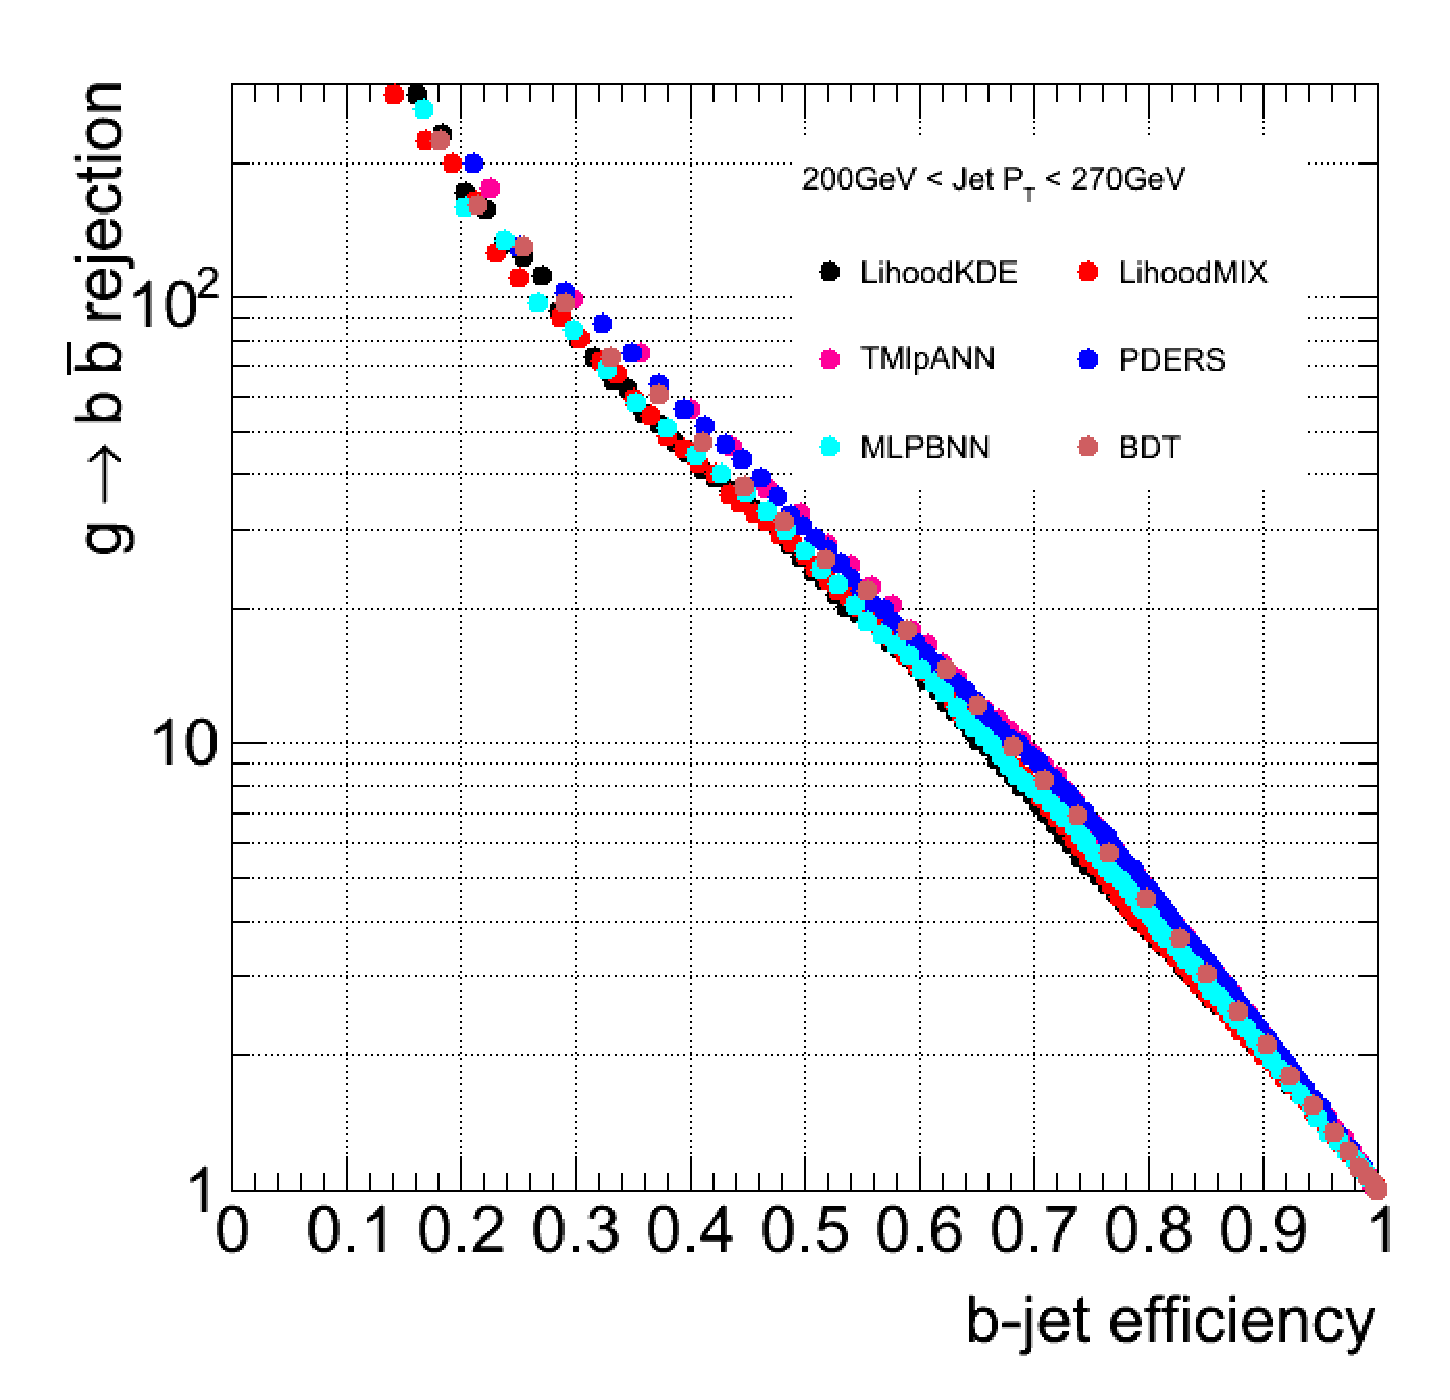
\includegraphics[width=0.49\textwidth]{FIGS/TEMPFigs/MVA_differentMethods/inclusive/MVAs_RejvsEff200.pdf}
\caption{Distribution of the MVA discriminant performance for inclusive training, in single and merged $b$-jets, for low and high jet $\pt$.}
\label{fig:diffmethodsPerfInclusive}
\end{figure}

\begin{figure}[tp]
\centering
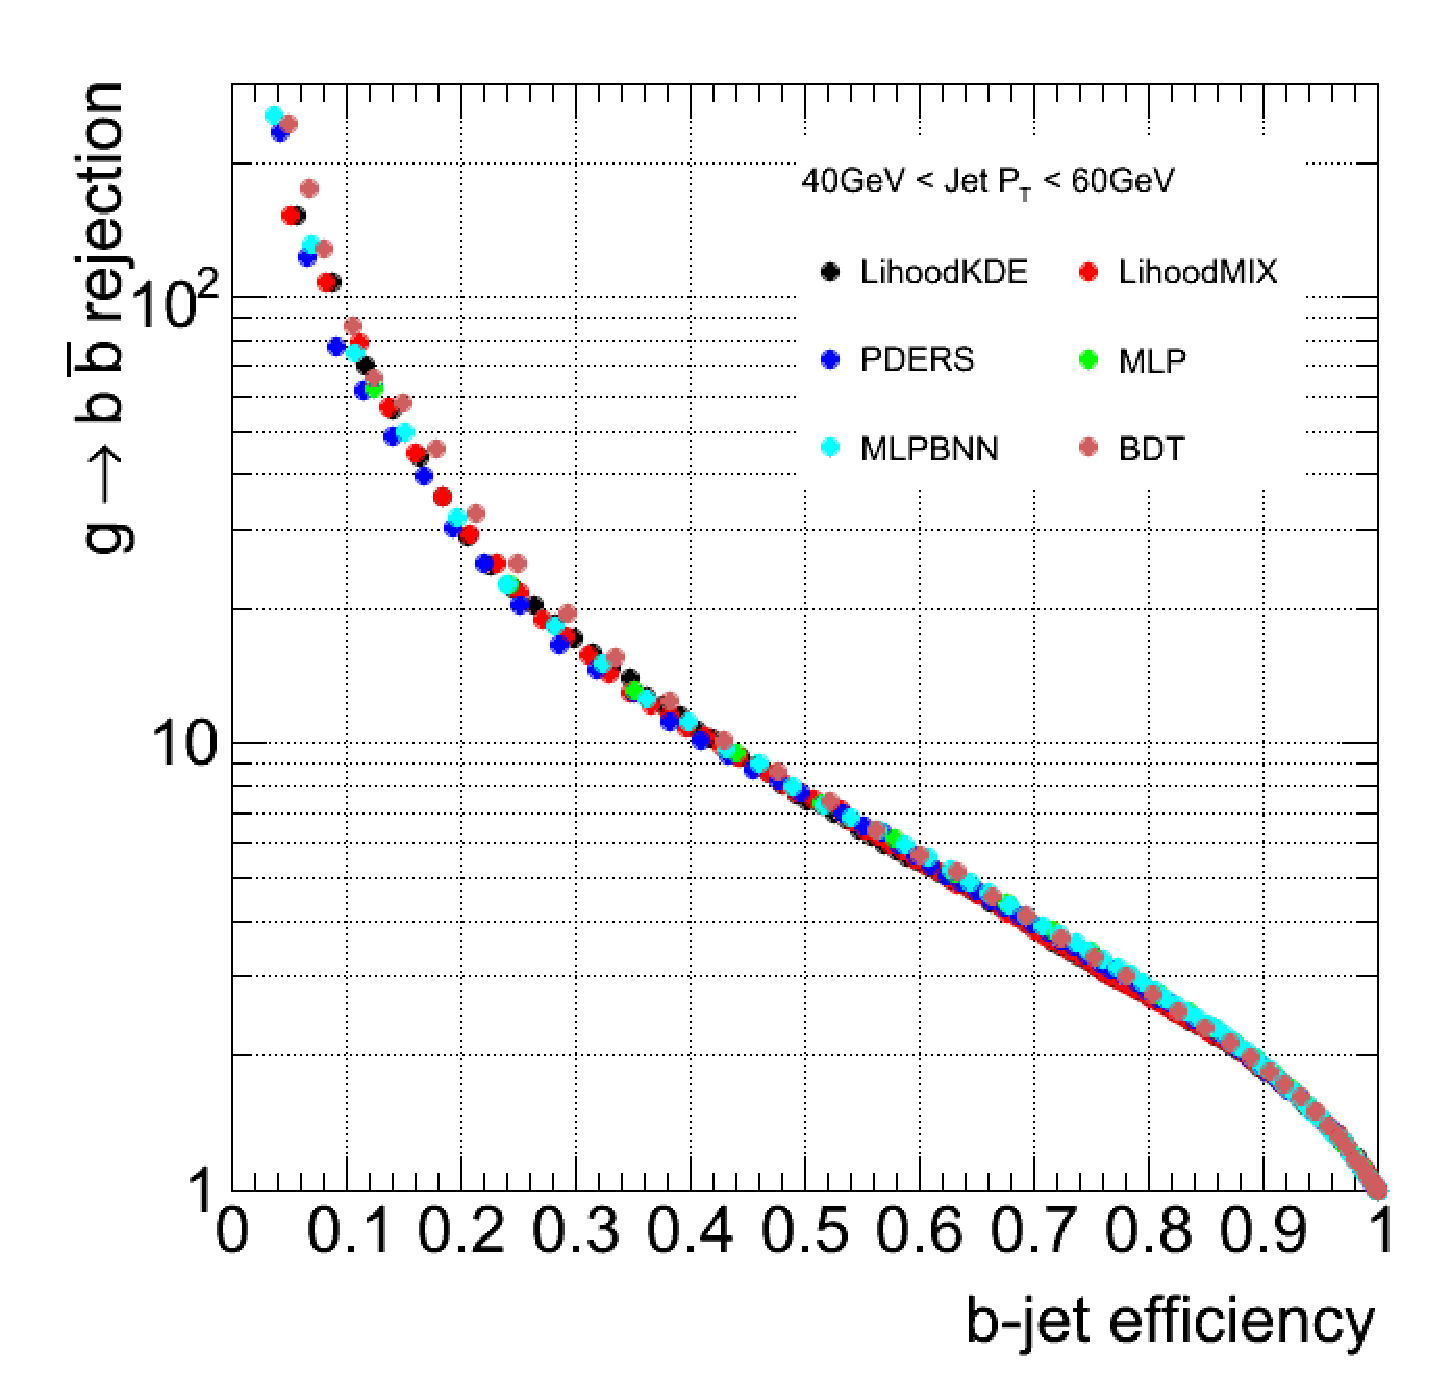
\includegraphics[width=0.49\textwidth]{FIGS/TEMPFigs/MVA_differentMethods/bins/MVAs_RejvsEff40.pdf}
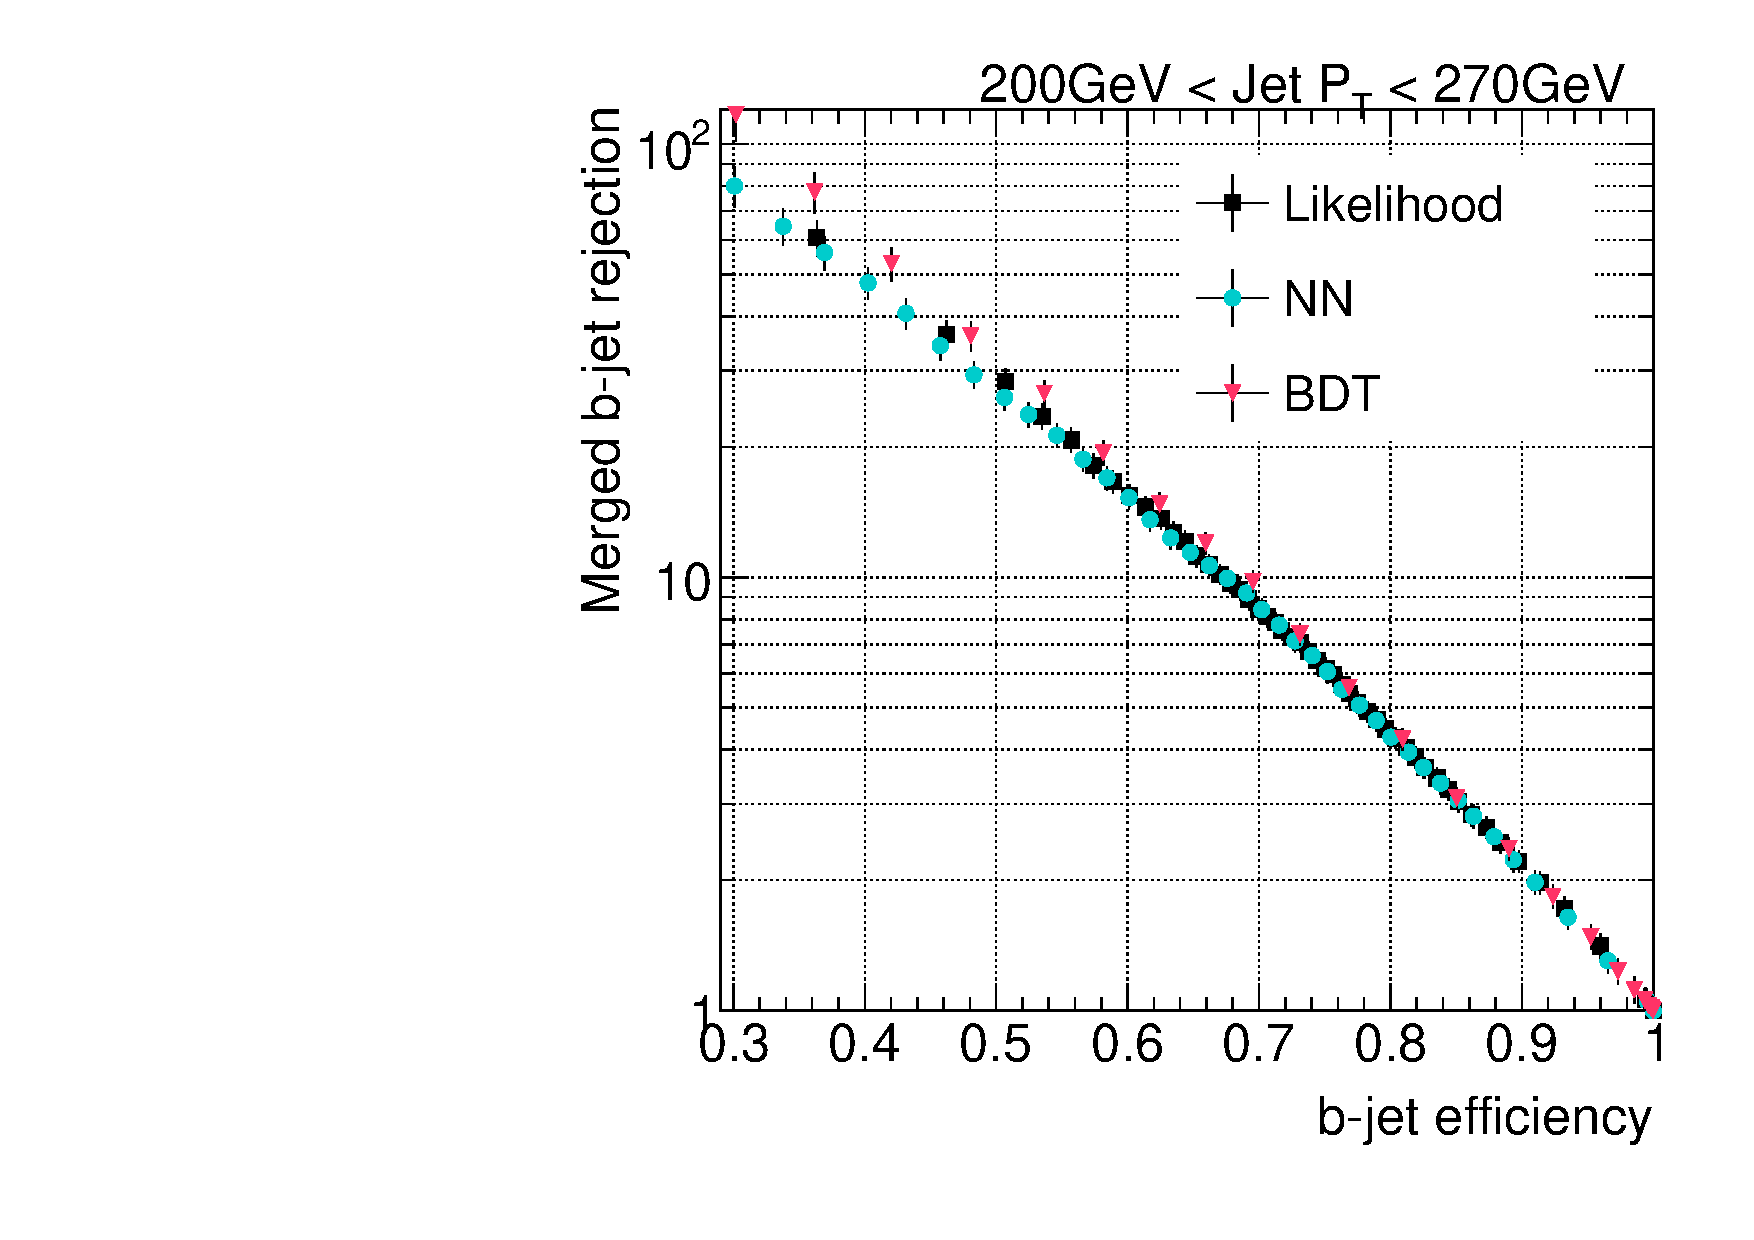
\includegraphics[width=0.49\textwidth]{FIGS/TEMPFigs/MVA_differentMethods/bins/MVAs_RejvsEff200.pdf}
\caption{Distribution of the MVA discriminant performance for training in bins of jet $\pt$, in single and merged $b$-jets, for low and high jet $\pt$.}
\label{fig:diffmethodsPerfBins}
\end{figure}



%------------------------------------------------------------------------
\section{$\bm{ g\rightarrow b\bar{b}}$ likelihood training and performance}
%------------------------------------------------------------------------

A discriminant between single $b$-jets and merged $b$-jets was built by training a simple likelihood estimator in the context of the Toolkit for Multivariate Data Analysis, TMVA~\cite{Hocker:2007ht}.

A sub-set of the dijet Monte Carlo sample was used for training. After the event and jet selections were performed, the $b$-tagged jets with $|\eta| < 2.1$ were classified as signal (single $b$-jets) or background (merged $b$). % depending on whether one or two $b$-hadrons were found within a 0.4 cone around the jet axis. %For the evaluation of the method the same procedure was followed.
The likelihood training was done in bins of calorimeter jet $\pt$. % and only isolated jets were considered. 
Signal and background jets were not weighted by the dijet samples cross-sections to allow the contribution of subleading lower \pt\ jets from high \pt\ events, and thus increase the statistics of merged jets in the low \pt\ bins. For the evaluation of the method the same procedure was followed.


%Several combinations of the tracking and jet shape variables studied in the previous section were tested as input variables. We found that the following combination of three variables offers the best performance:
As mentioned in the previous section, the following combination of three variables was chosen for the multivariate analysis:
\begin{enumerate}\addtolength{\itemsep}{-0.4\baselineskip}
\item
Jet track multiplicity
\item
Track-jet width
\item
$\Delta R$ between the axes of 2 $k_t$ subjets within the jet
\end{enumerate}
%
%A requirement of at least two matching tracks was imposed to all $b$-tagged jets in order to build the third variable listed. This cut was applied in both training and testing samples.

The distribution of the likelihood output for single and merged $b$-jets is shown in  Fig.~\ref{fig:outputinbins} for low, medium and high transverse momentum jets.

\begin{figure}[tp]
\centering
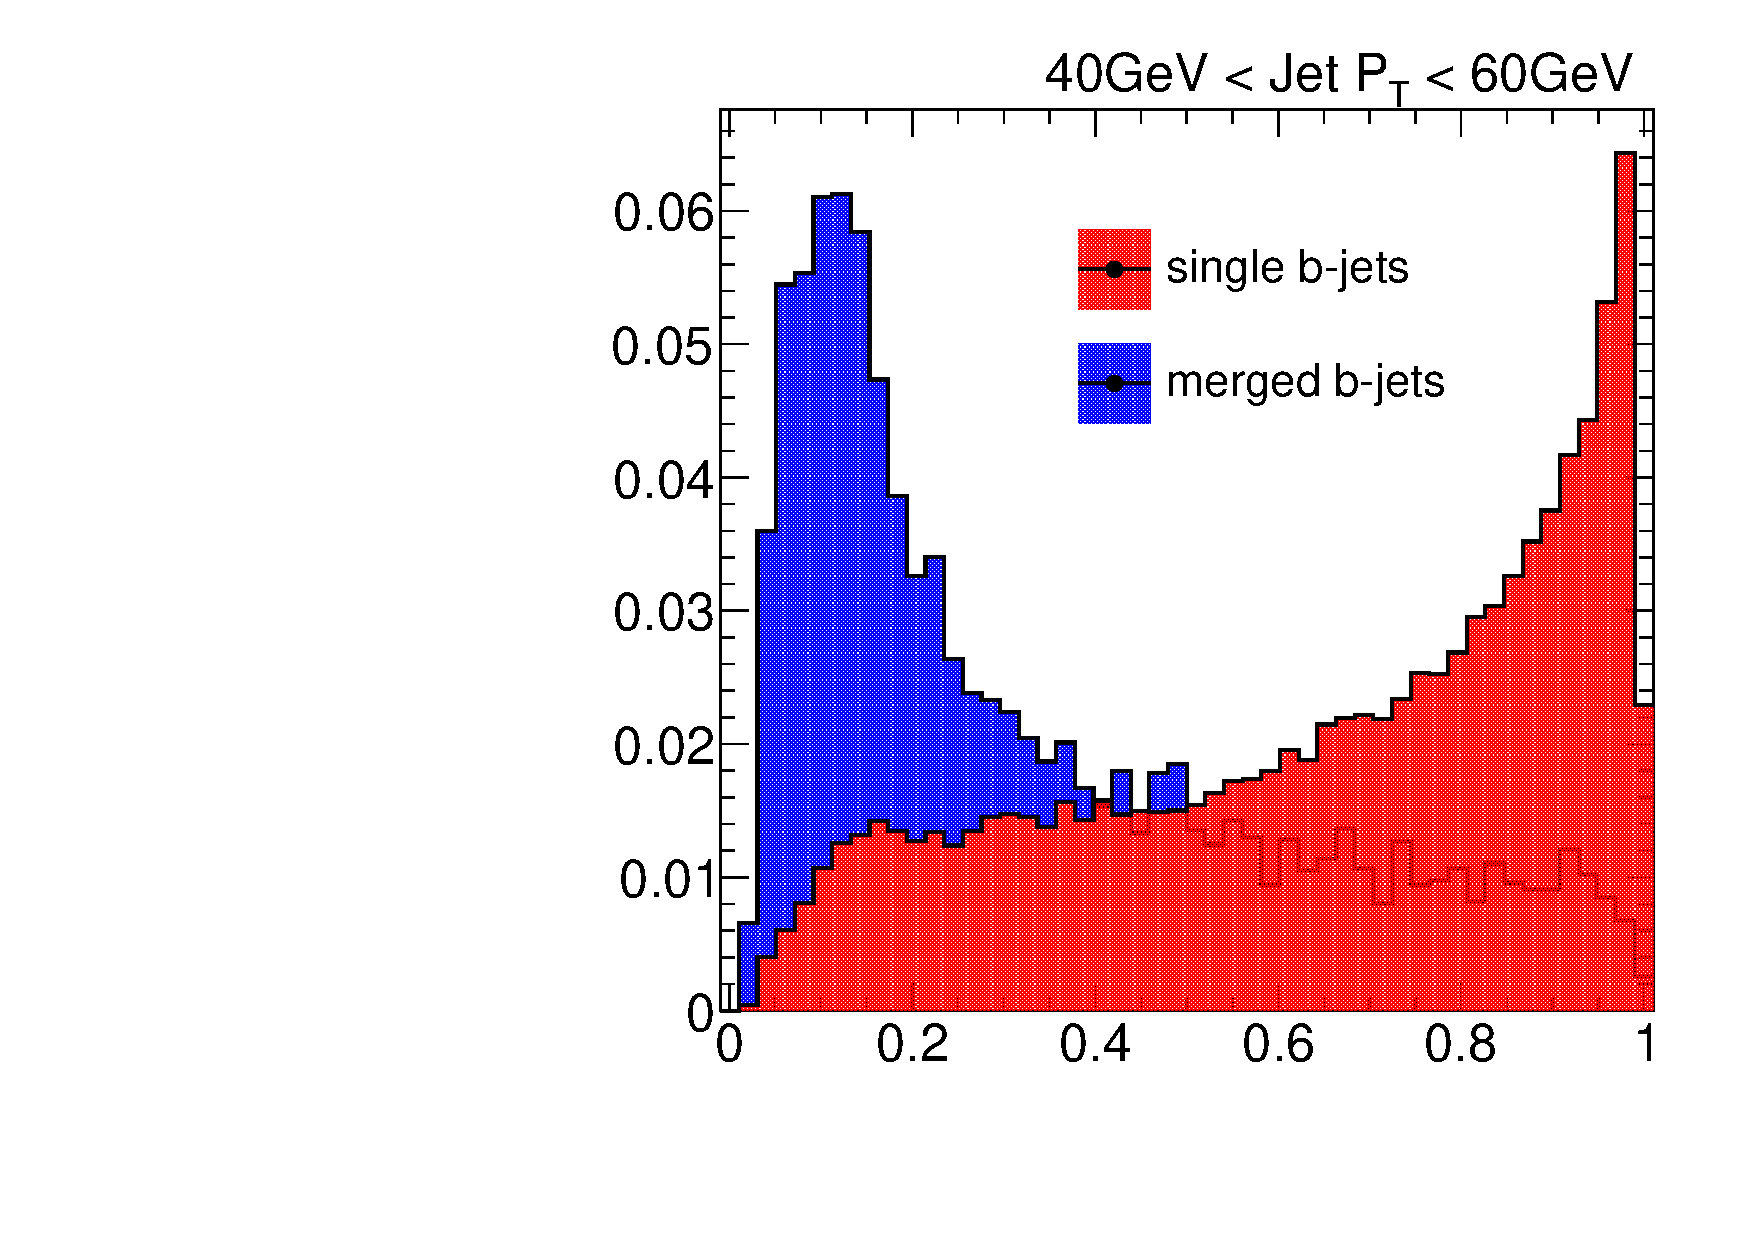
\includegraphics[width=0.32\textwidth,viewport=40 0 540 550]{FIGS/Likelihood/NNoutput040_LihoodKDE.pdf}
%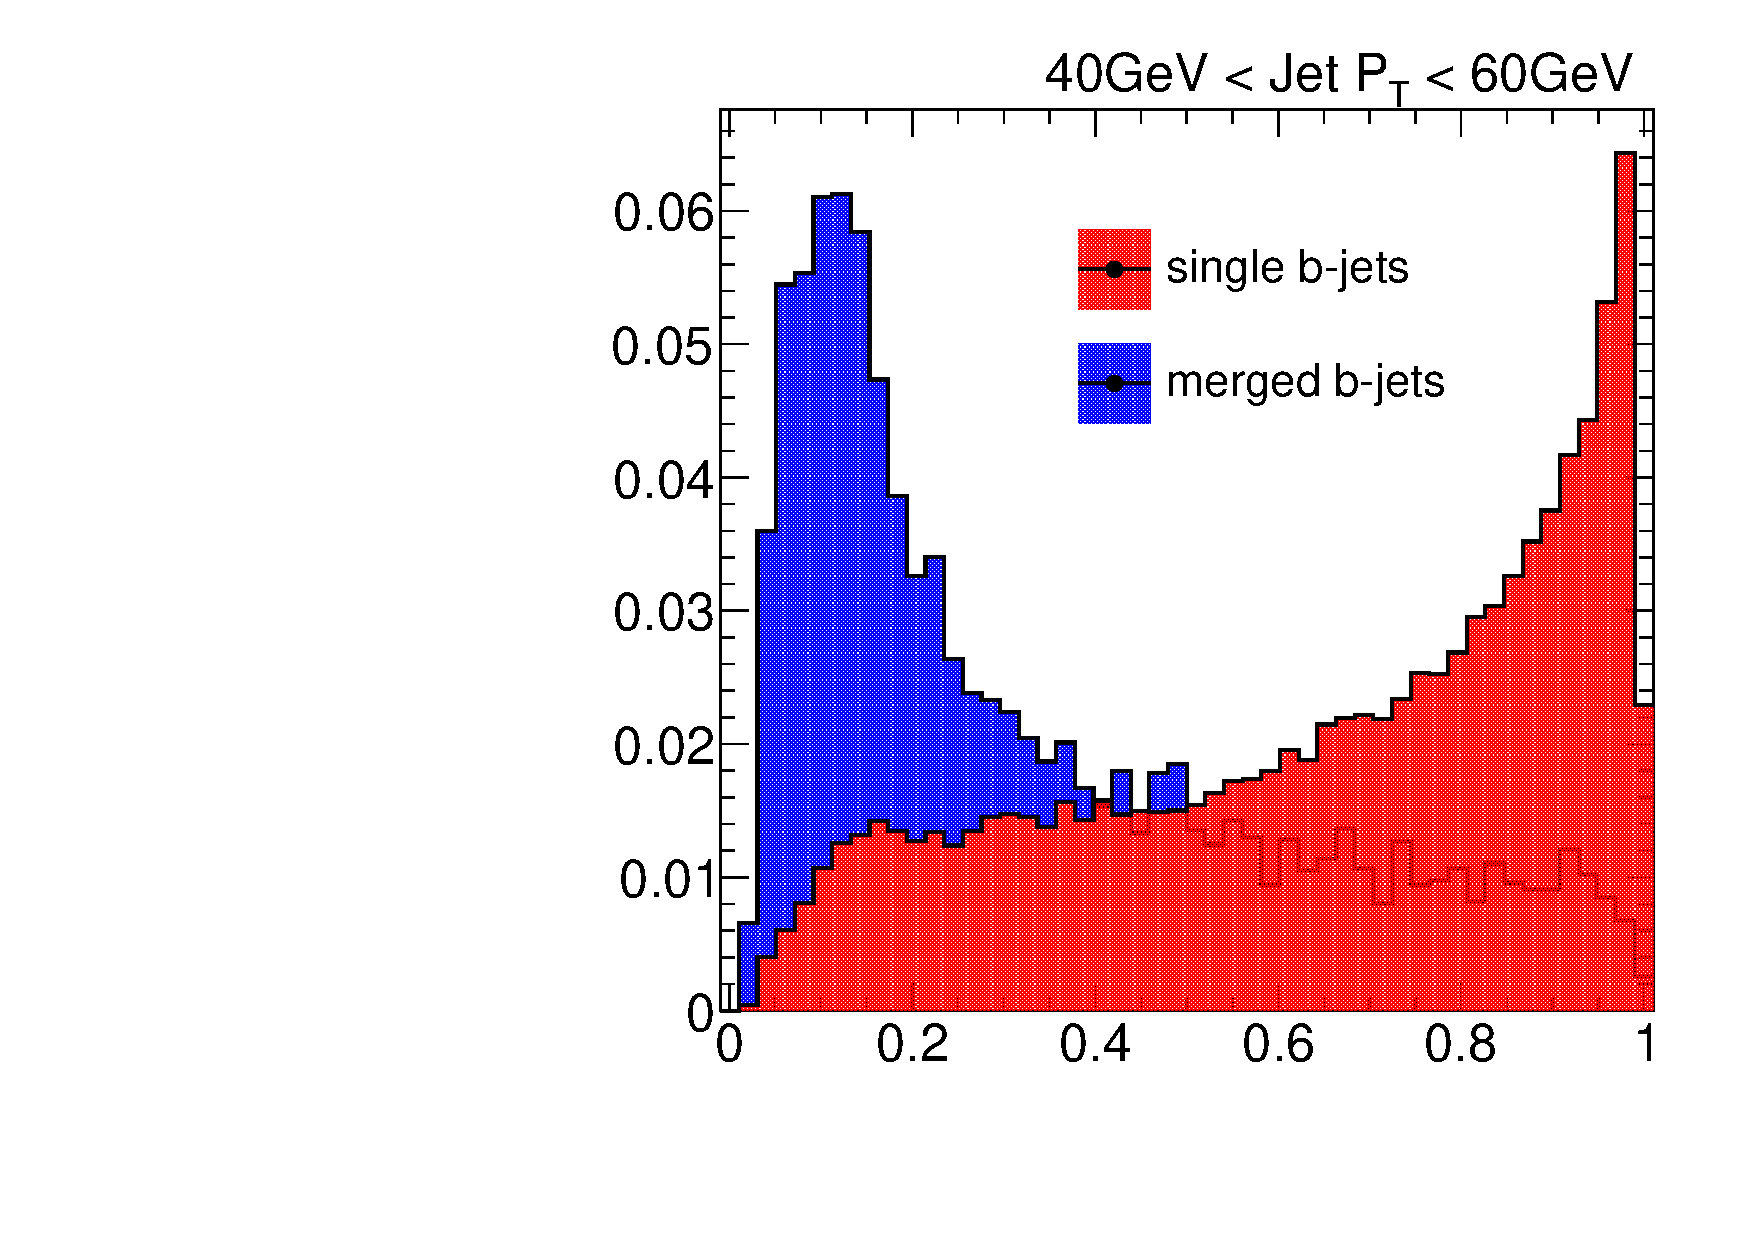
\includegraphics[width=0.32\textwidth]{FIGS/Likelihood/NNoutput040_LihoodKDE.pdf}
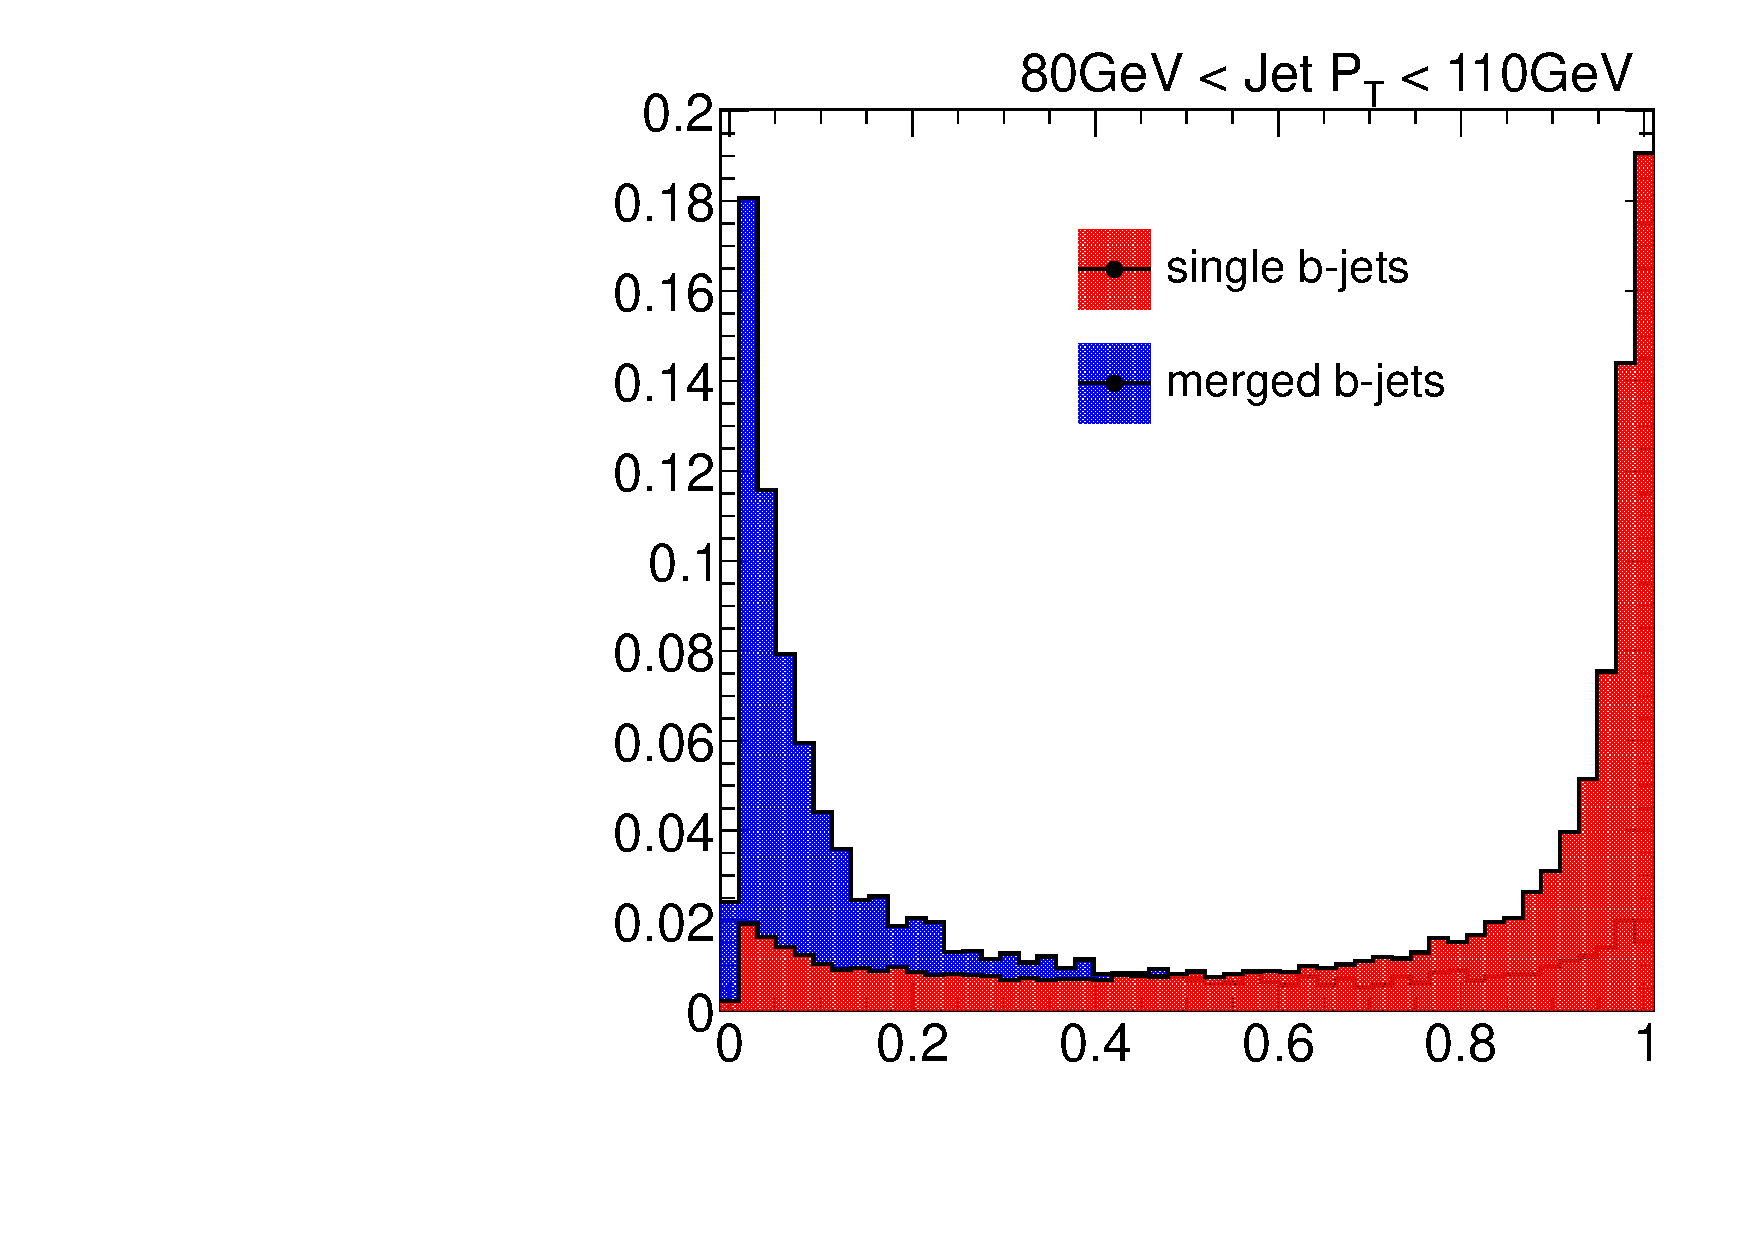
\includegraphics[width=0.32\textwidth,viewport=40 0 540 550,clip]{FIGS/Likelihood/NNoutput080_LihoodKDE.pdf}
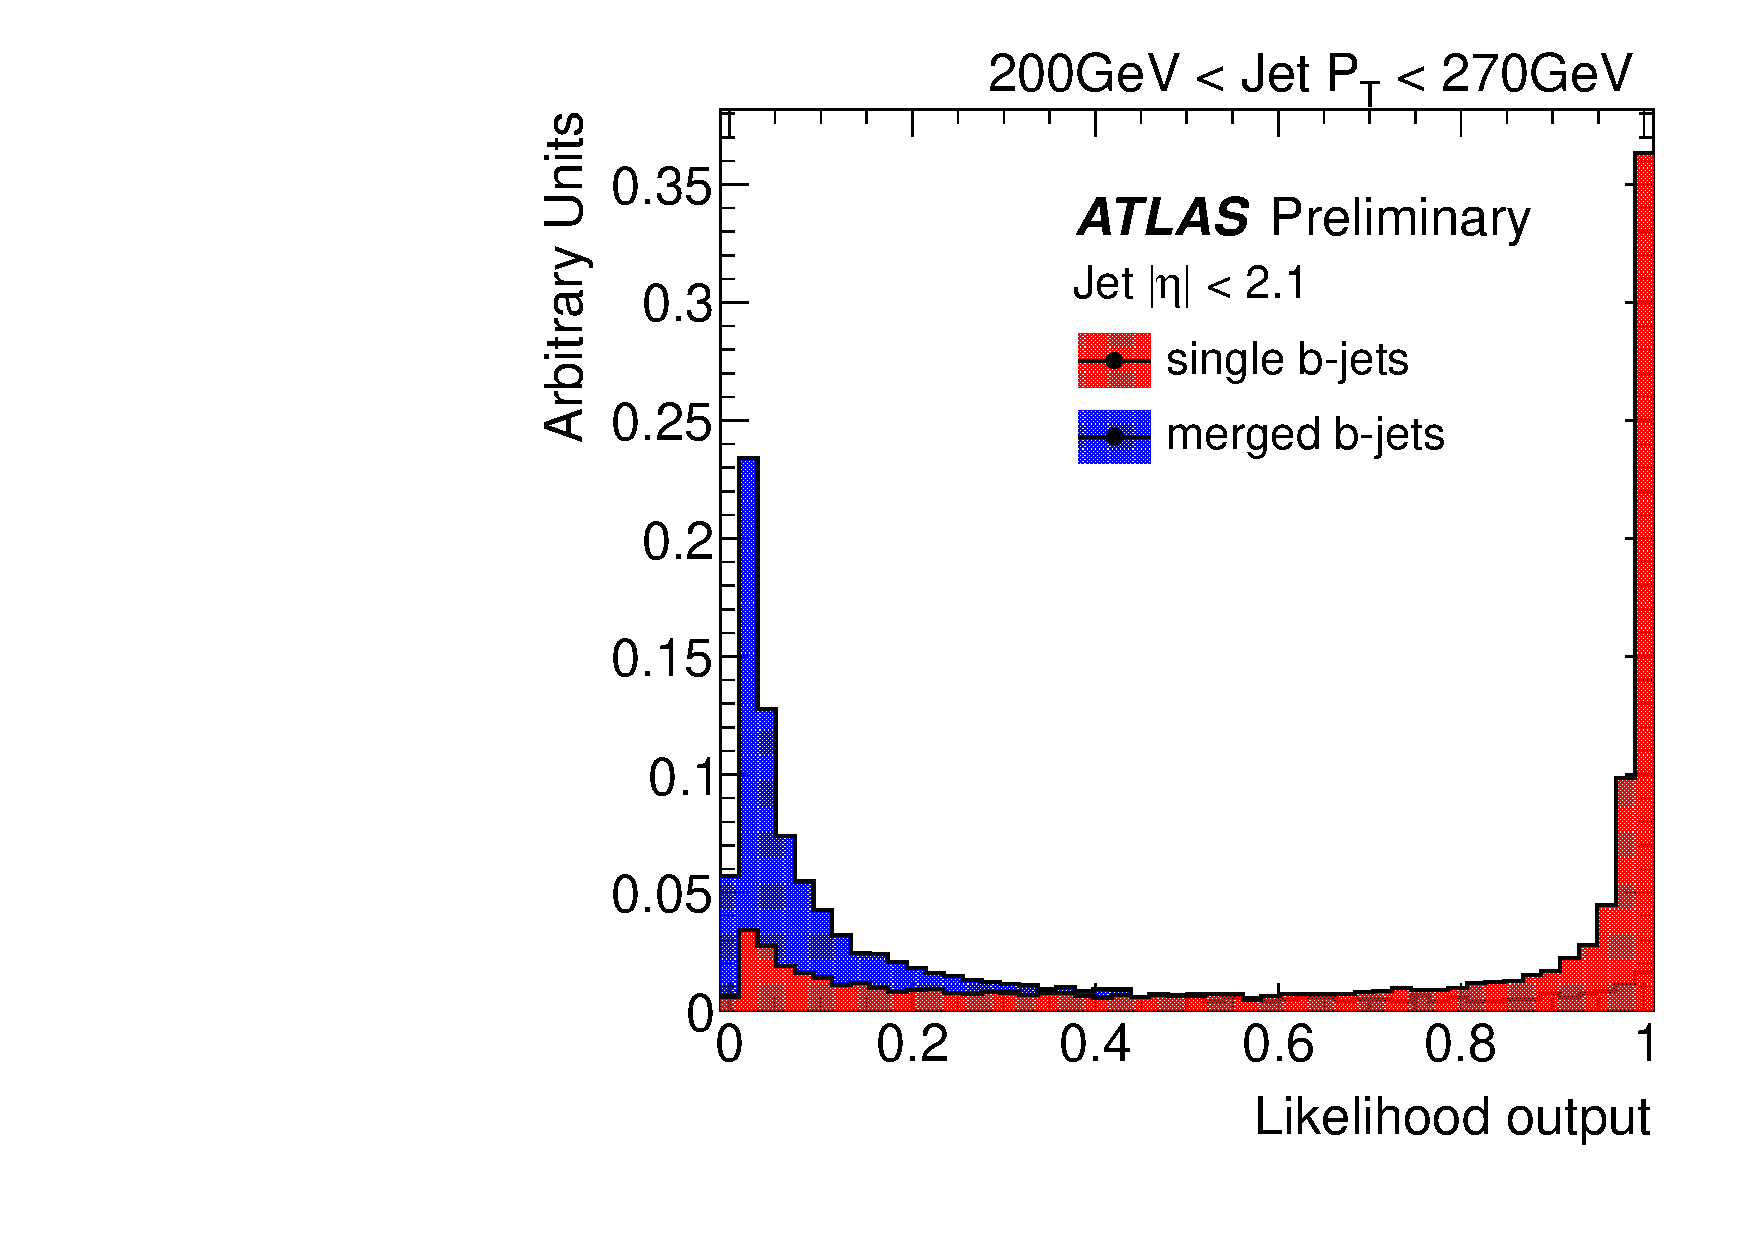
\includegraphics[width=0.32\textwidth,viewport=40 0 540 550,clip]{FIGS/Likelihood/NNoutput200_LihoodKDE.pdf}  
\caption{Distribution of the likelihood output for single and merged $b$-jets for low, medium and high $\pt$ jets.}
\label{fig:outputinbins}
\end{figure}

The performance of the tagger in the simulation can be  %seen in Fig.~\ref{fig:performanceinbins}. In this plot the rejection ($1/\epsilon_{bkg}$) of merged $b$-jets from gluon splitting is shown as a function of single $b$-jet efficiency for the eight bins of jet $\pt$ mentioned in section~\ref{sec:EventSelection}. The performance improves with $\pt$:
displayed in a plot of rejection ($1/\epsilon_{bkg}$) of merged $b$-jets as a function of single $b$-jet efficiency, where $\epsilon_{bkg}$ is the probability that a double $b$-hadron jet passes the single $b$-jet tagger. This is shown in Fig.~\ref{fig:performanceinbins} for the eight bins of jet $\pt$ mentioned in section~\ref{sec:EventSelection}. The performance improves with $\pt$:


\begin{itemize}\addtolength{\itemsep}{-0.4\baselineskip}
\item
$\pt>40$ GeV: %\\[1mm]
rejection above 8 at 50\% eff.
% over 85\% rejection at 50\% eff.
\item
$\pt>60$ GeV: %\\[1mm]
rejection above 10 at 50\% eff.
 %90\% rejection at 50\% eff.
\item
$\pt>200$ GeV: %\\[1mm]
rejection above 30 at 50\% eff.
 %over 95\% rejection at 50\% eff.
\end{itemize}


\begin{figure}[tp]
\centering
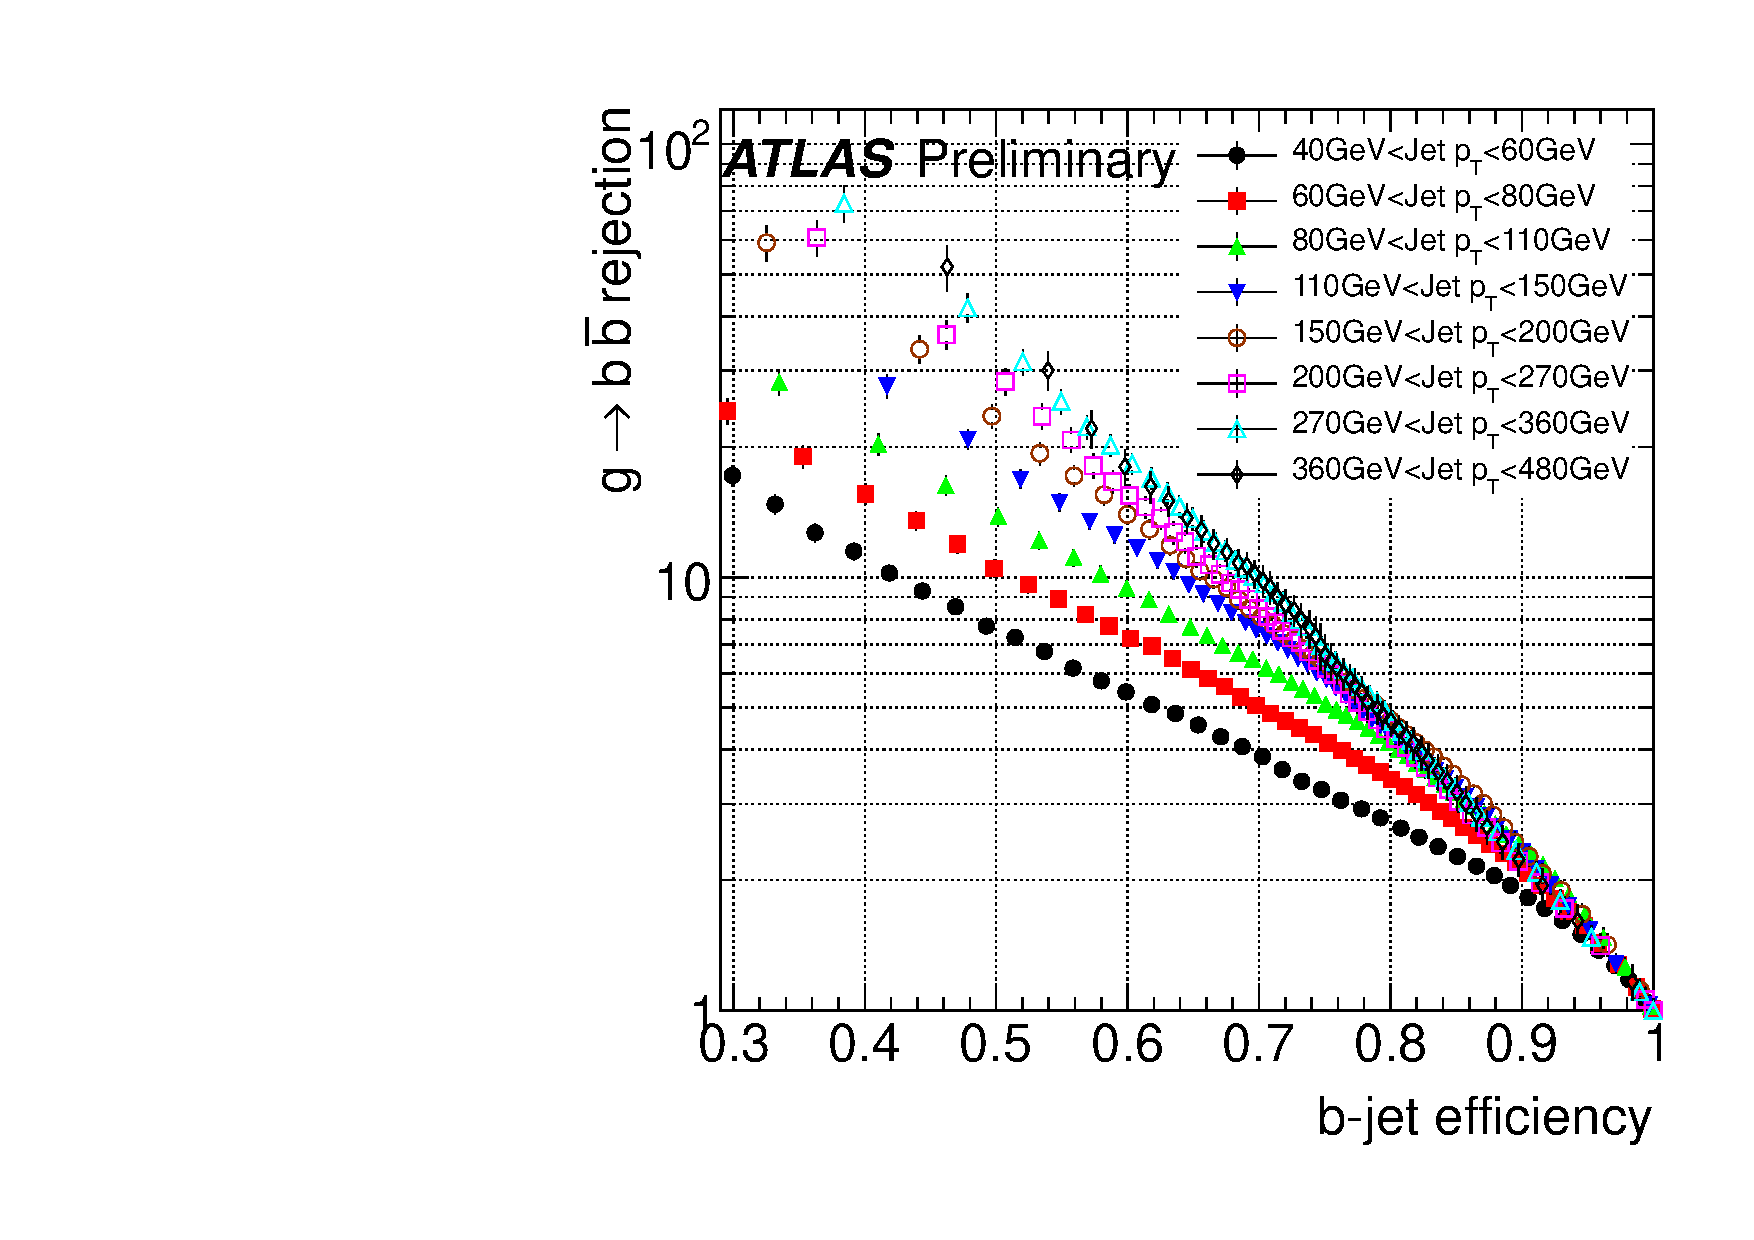
\includegraphics[width=0.7\textwidth]{FIGS/Likelihood/KDE_RejvsEff.pdf}
\caption{Rejection of merged $b$-jets as a function of single $b$-jet efficiency for dijet events in 8 jet $\pt$ bins.}
\label{fig:performanceinbins}
\end{figure}


The rejection of merged jets attained as a function of \pt\ for the 50\% and 60\% single $b$-jet efficiency working points are summarized in Table~\ref{tb:rejection}, together with their relative statistical error. These are propagated from the Poisson fluctuations of the number of events in the merged and single $b$ distributions. The error is slightly lower for the 60\% efficiency working point because a higher efficiency allows for a greater number of Monte Carlo events to measure the performance. %the higher the efficiency, the larger the number of Monte Carlo events available to measure the performance.




\begin{table}[!hbt] %[h]
\renewcommand{\arraystretch}{1.2}
\centering
\begin{tabular}{ | c || c | c || c | c||}
  \hline
  Jet \pt & \multicolumn{2}{c||}{single $b$-jet efficiency 50\%} & 
            \multicolumn{2}{c||}{single $b$-jet efficiency 60\%}\\ \cline{2-5}
    (GeV )  & Rejection & ~stat.err.~ & Rejection & ~stat.err.~ \\ \hline
%   40 - 60 &  ~7.6 &  4\%  &  ~5.4  &  3\%    \\ 
%   60 - 80 &  10.4 &  4\%  &  ~7.3  &  4\%    \\ 
%   80 - 110&  13.9 &  5\%  &  ~9.4  &  4\%    \\ 
%  110 - 150&  18.7 &  5\%  &  12.0  &  4\%    \\ 
%  150 - 200&  23.2 &  5\%  &  14.0  &  5\%    \\ 
%  200 - 270&  29.5 &  7\%  &  15.6  &  6\%    \\ 
%  270 - 360&  36.4 &  7\%  &  18.7  &  6\%    \\ 
%  360 - 480&  41.4 &  8\%  &  18.2  &  8\%    \\ \hline
   40 - 60 &  ~8 &  4\%  &  ~5  &  3\%    \\ 
   60 - 80 &  ~10 &  4\%  &  ~7  &  4\%    \\ 
   80 - 110&  ~14 &  5\%  &  ~9  &  4\%    \\ 
  110 - 150&  19 &  5\%  &  12  &  4\%    \\ 
  150 - 200&  23 &  5\%  &  14  &  5\%    \\ 
  200 - 270&  30 &  7\%  &  16  &  6\%    \\ 
  270 - 360&  36 &  7\%  &  19  &  6\%    \\ 
  360 - 480&  41 &  8\%  &  18  &  8\%    \\ \hline
\end{tabular}
\caption{The merged $b$-jet rejection for the 50\% and 60\% efficiency working points in bins of $\pt$.}
\label{tb:rejection}
\end{table}





%------------------------------------------------------------------------
\section{Systematic uncertainties}\label{sec:gbbSystematics}
%------------------------------------------------------------------------
The development, training and performance determination of the tagger is based on simulated events. Although the agreement between simulation and data explored in section~\ref{sec:validation} is a necessary validation condition, it is also important to investigate how the tagger performance depends on systematics relevant in the data. In particular we have considered:
%
%There are uncertainties in the data that, although not spoiling the data/MC agreement, might change the performance of the tagger. This uncertainties would also be present in an eventual future data-driven determination of the performance as  the data are not known better that this.The following systematic effects have been studied and their influence on the tagger performance ascertained:
%
%In order to study the systematic uncertainties in the method the following contributions were evaluated:
\begin{itemize}\addtolength{\itemsep}{-0.4\baselineskip}
\item
presence of additional interactions (pile-up);
\item
uncertainty in the $b$-jet tagging efficiency; % and b-jet energy scale?
\item
uncertainty in the track reconstruction efficiency;
\item
uncertainty in the track transverse momentum resolution;
\item
uncertainty in the jet transverse momentum resolution;
\item
uncertainty in the $b$-jet energy scale.
%the effect of jet isolation
%\item
%other $\Delta R$ cuts for B-labeling and matching
\end{itemize}

{ \em I. Pile-up}
\\[3mm]
  The size of this effect was studied by comparing the performance of the likelihood discriminant with $b$-jets in events with small (1-9) and large (9-20) number of primary vertices. 
%The comparison of the performance in these two sub-samples can be seen in Fig.~\ref{fig:performanceinbinsMu}. 
As expected from the use of tracking (as opposed to calorimeter) variables no significant dependence with pile-up is observed within statistics. %Of the 16 determinations (2 working points with 8 \pt\ bins each) of performance differences between high and low number of primary vertices events, it is observed that 6 of them are positive and 10 negative, with a global mean of 0.3\%. We conclude that the effect is negligible compared to other source of uncertainties.
Performance differences between high and low number of primary vertices events are $\leq$~0.3\% and therefore negligible compared to other sources of uncertainties. The impact of pile-up might be larger in 2012.

%

%\begin{figure}[tp]
%\centering
%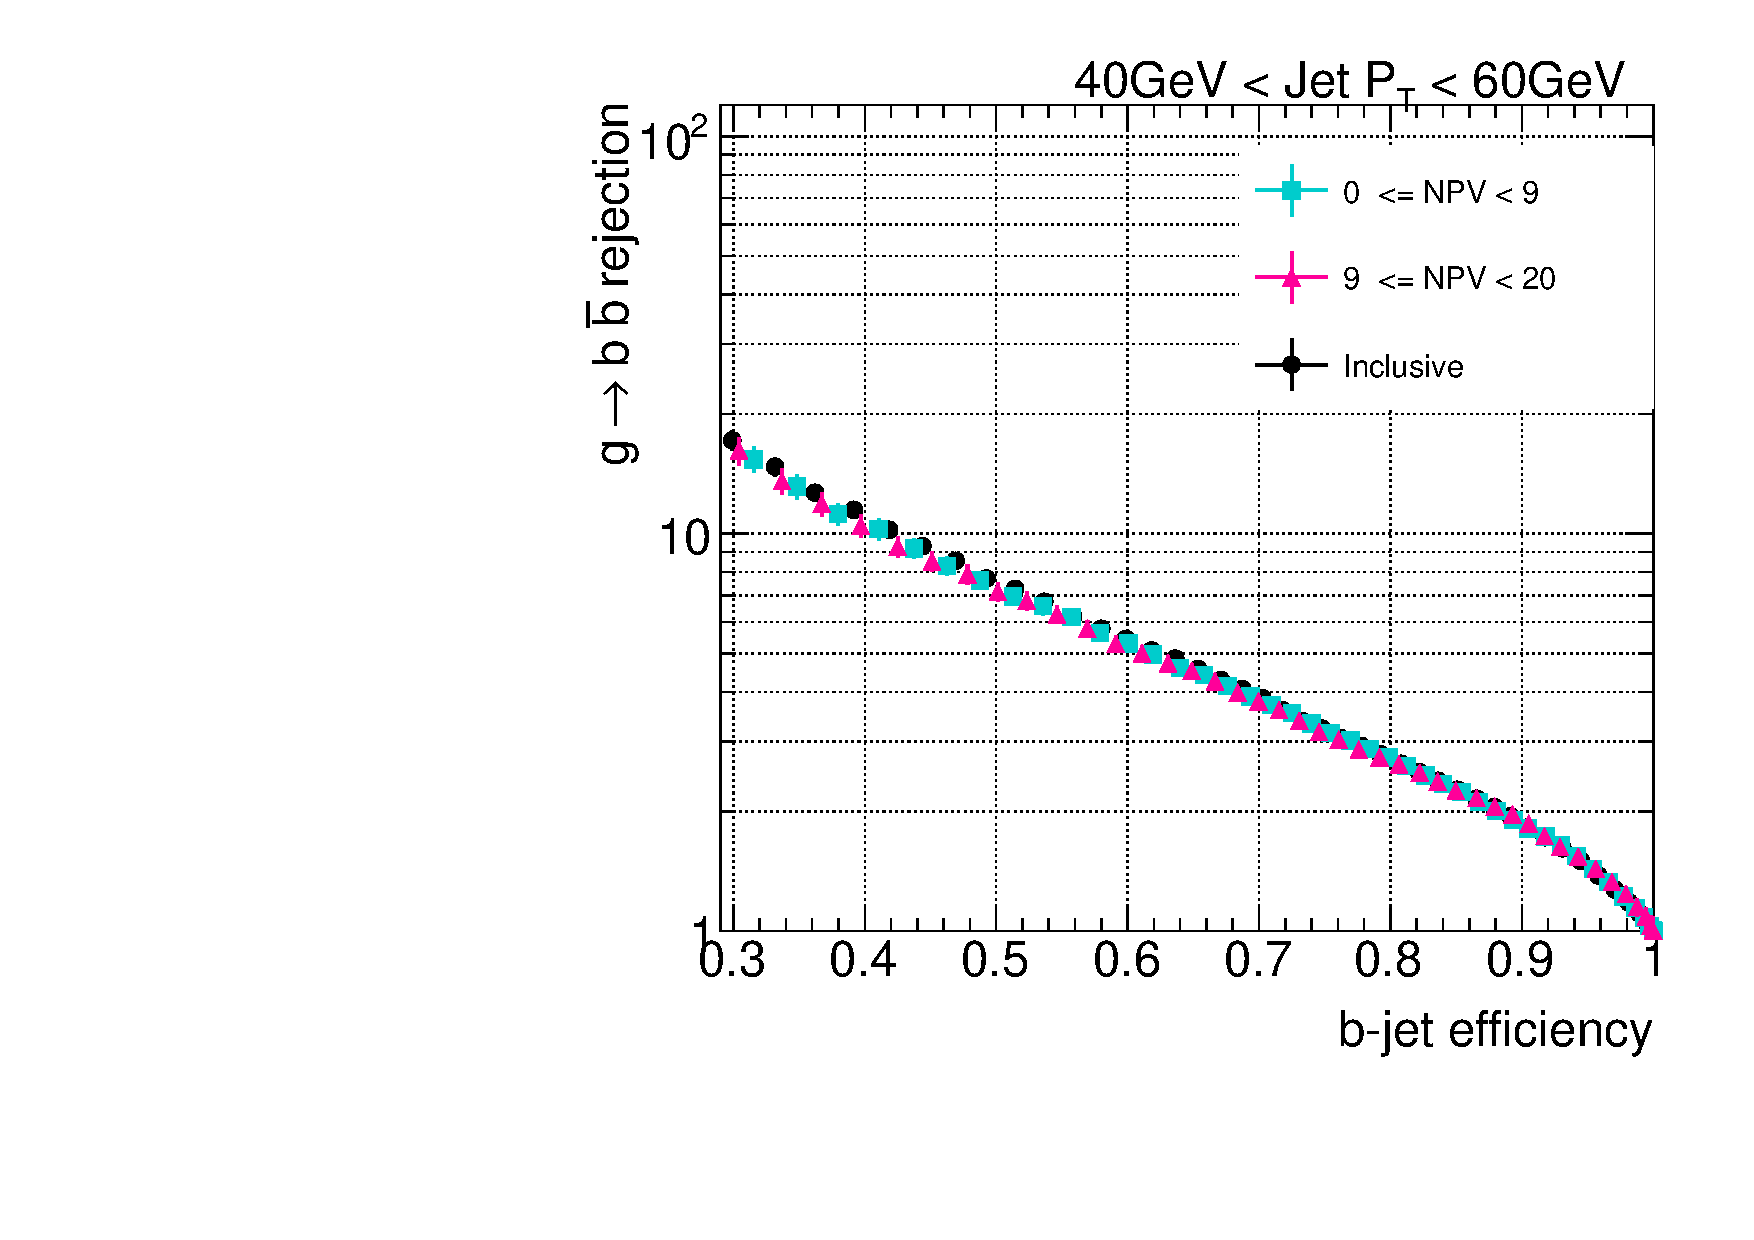
\includegraphics[width=0.49\textwidth]{FIGS/systematics/50BinsLlhoodKDE_ISO_PileUp_rejvseff040.pdf}
%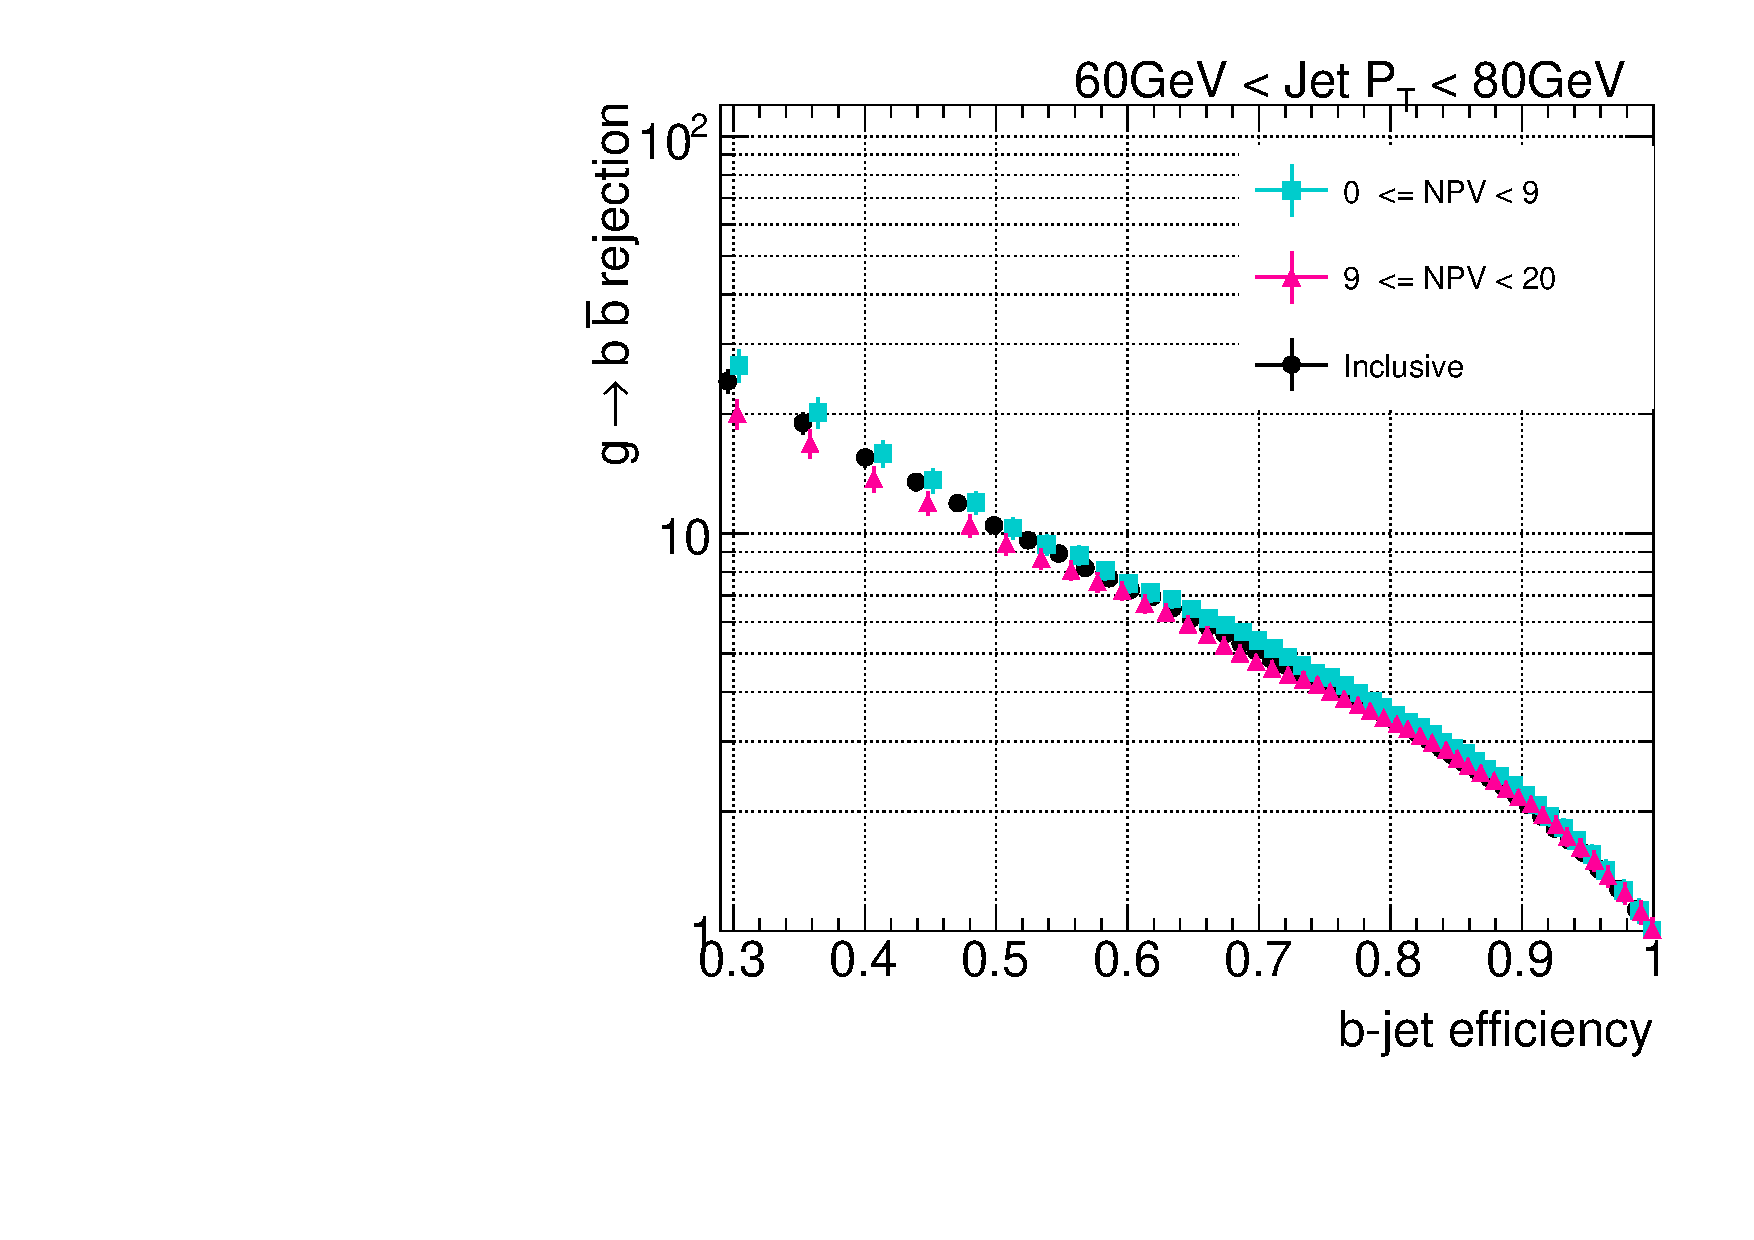
\includegraphics[width=0.49\textwidth]{FIGS/systematics/50BinsLlhoodKDE_ISO_PileUp_rejvseff060.pdf}
%\caption{Rejection of $g\rightarrow b \bar{b}$ merged b-jets as a function of $b$-jet efficiency in bins of $N_{\rm vtx}$ for two low jet $\pt$ bins.}
%\label{fig:performanceinbinsMu}
%\end{figure}

\vspace{3mm}
{\em II. b-tagging efficiency} %energy scale and 
\\[3mm]
The performance of heavy-flavor tagging in Monte Carlo events is calibrated to experimental data by means of the scale factors (SFs). %measured by the $b$-tagging group. 
These are defined as the ratio of the heavy-flavor tagging efficiency in data over that in Monte Carlo for the different jet flavors. They are measured by the $b$-tagging group,  %, and probably also as a function of jet pT and η 
%Such a measurement carries a systematic uncertainty, and in order to estimate its effect a conservative approach is followed: %https://twiki.cern.ch/twiki/bin/viewauth/AtlasProtected/BTaggingCalibrationDataInterface
and their measurement carries a systematic uncertainty.  

To estimate the impact of this uncertainty a conservative approach is followed: the SFs are varied in all the $\pt$ bins simultaneously by one standard deviation both in the up and down directions. The MC distributions weighted by the varied SFs show no major deviations from the nominal.  %The result of this procedure for the distribution of two of the tracking variables used in our discriminant is illustrated in Fig.~\ref{fig:btaggingSFs}. 
In the same manner, the effect of the $b$-tagging calibration uncertainty on the likelihood peformance is $< 1$\%, negligible with respect to the statistical uncertainty.
% as it can be seen in Fig.~\ref{fig:btaggingSFsPerf}.
This was indeed expected. The scale factors depend on the true flavor of the jet and on its \pt, but these are basically constant in the performance determination, which is based on single flavor (true $b$-) jets classified in \pt-bins.


%\begin{figure}[tp]
%\centering
%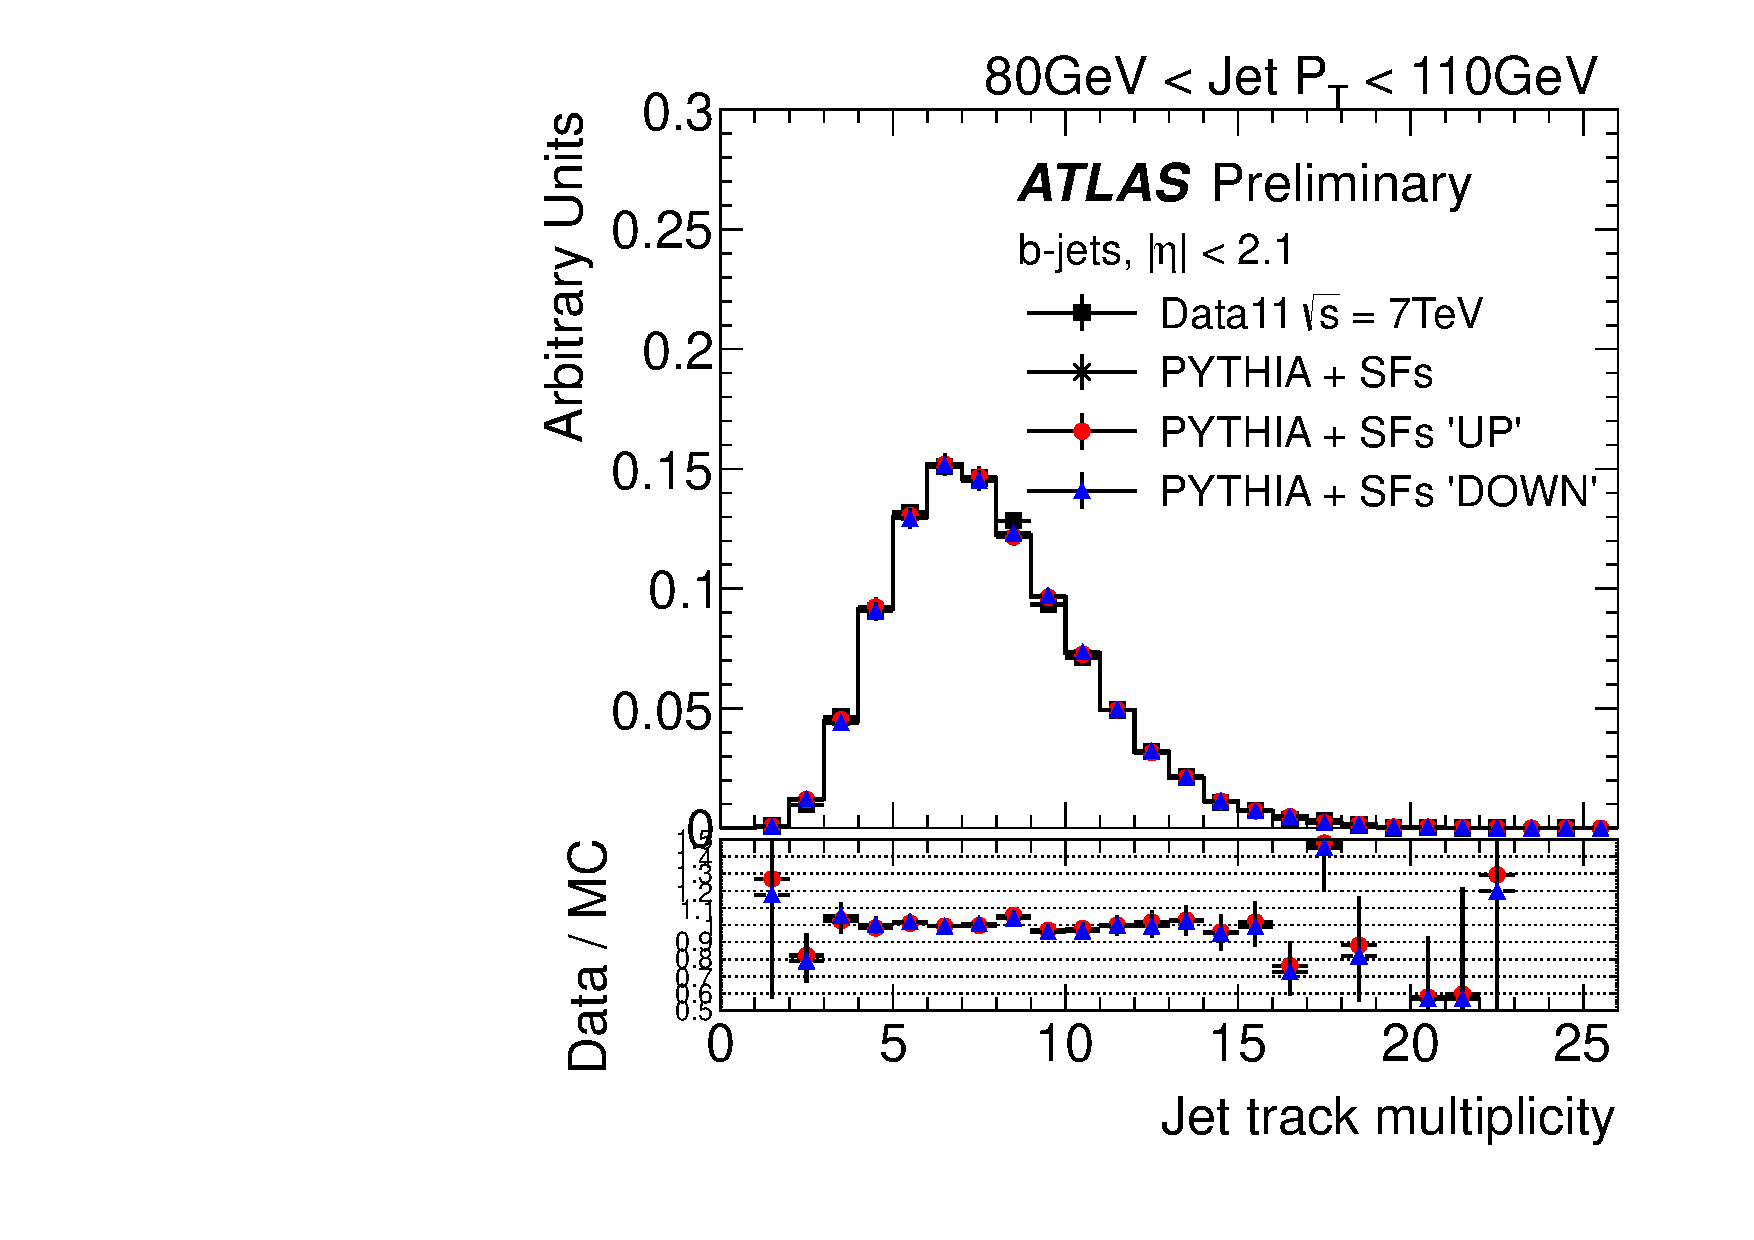
\includegraphics[width=0.49\textwidth]{FIGS/systematics/BTagCalib_DataVarNtrkPT080.pdf}
%%%%%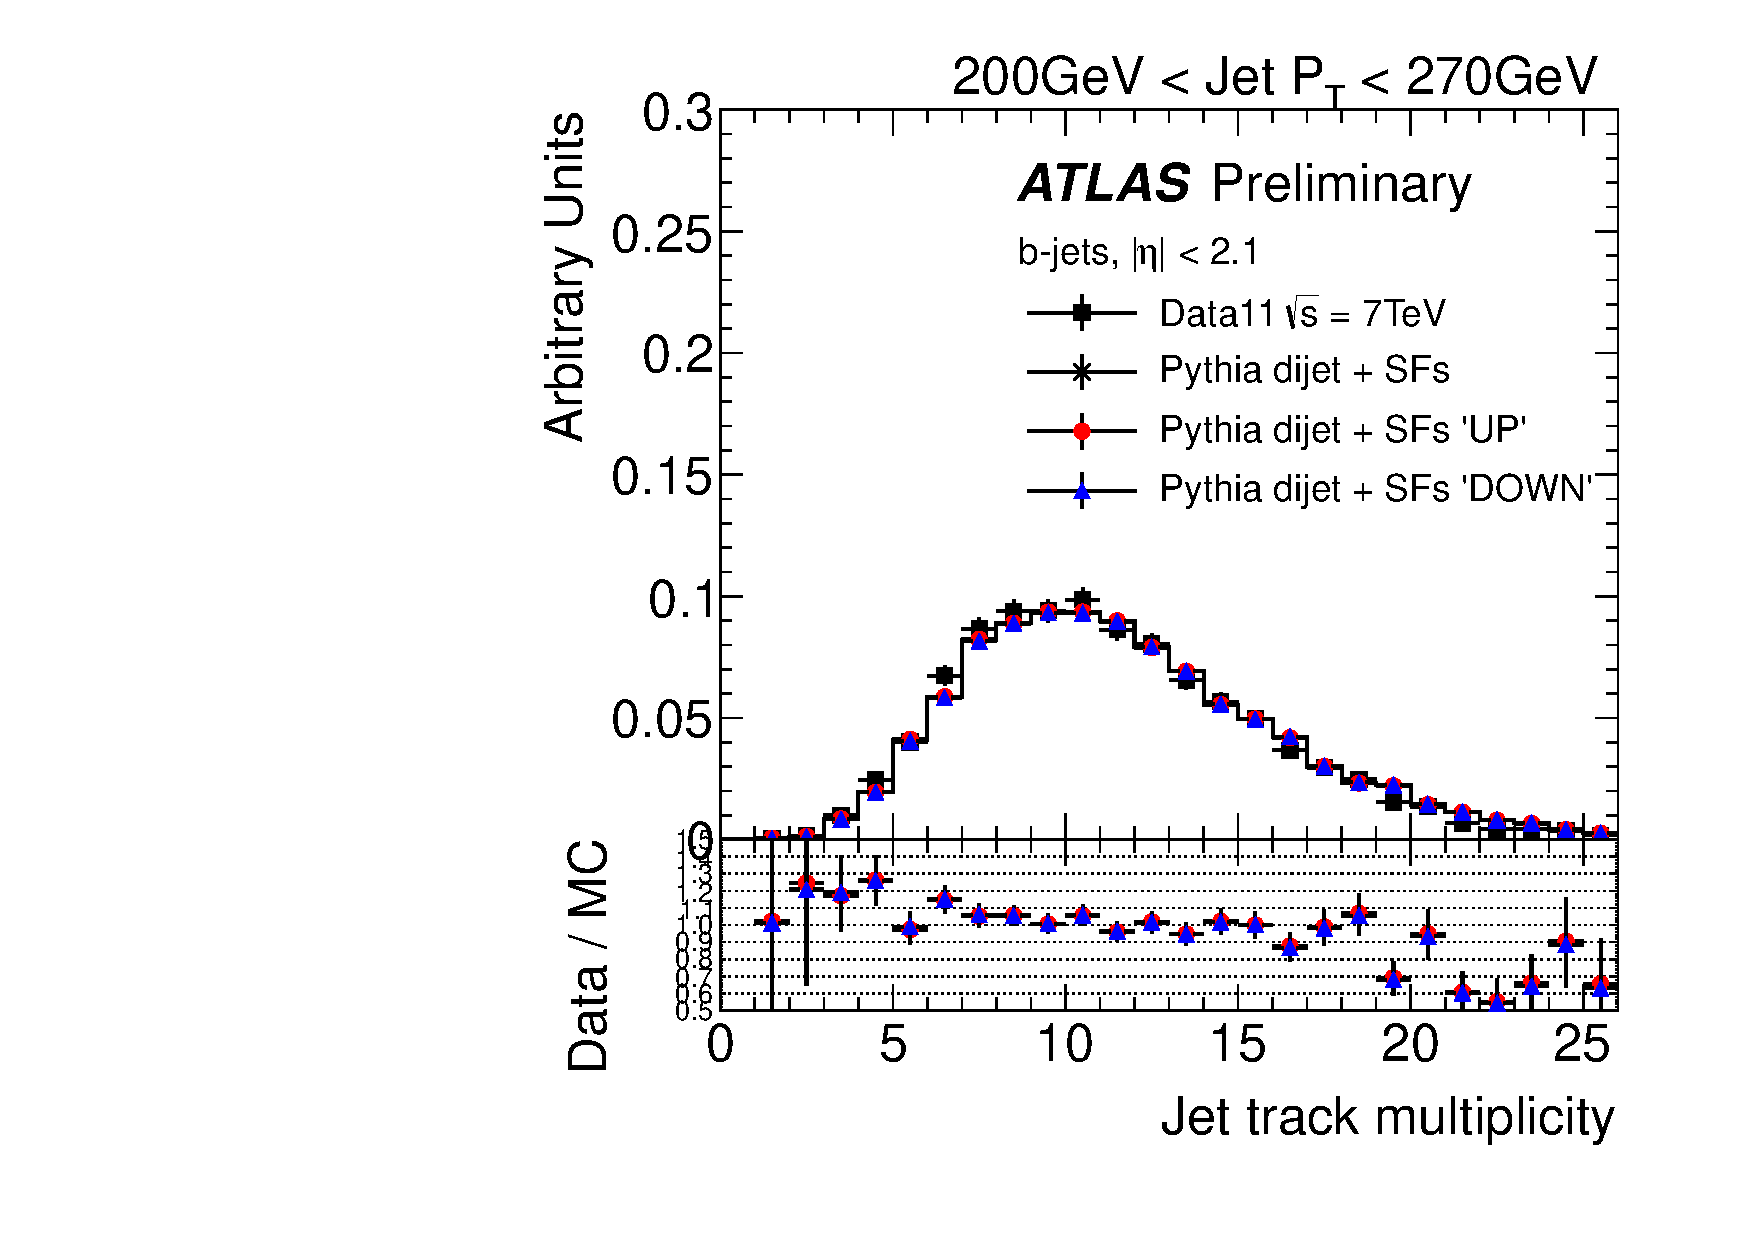
\includegraphics[width=0.49\textwidth]{FIGS/systematics/BTagCalib_DataVarNtrkPT200.pdf}
%%%%%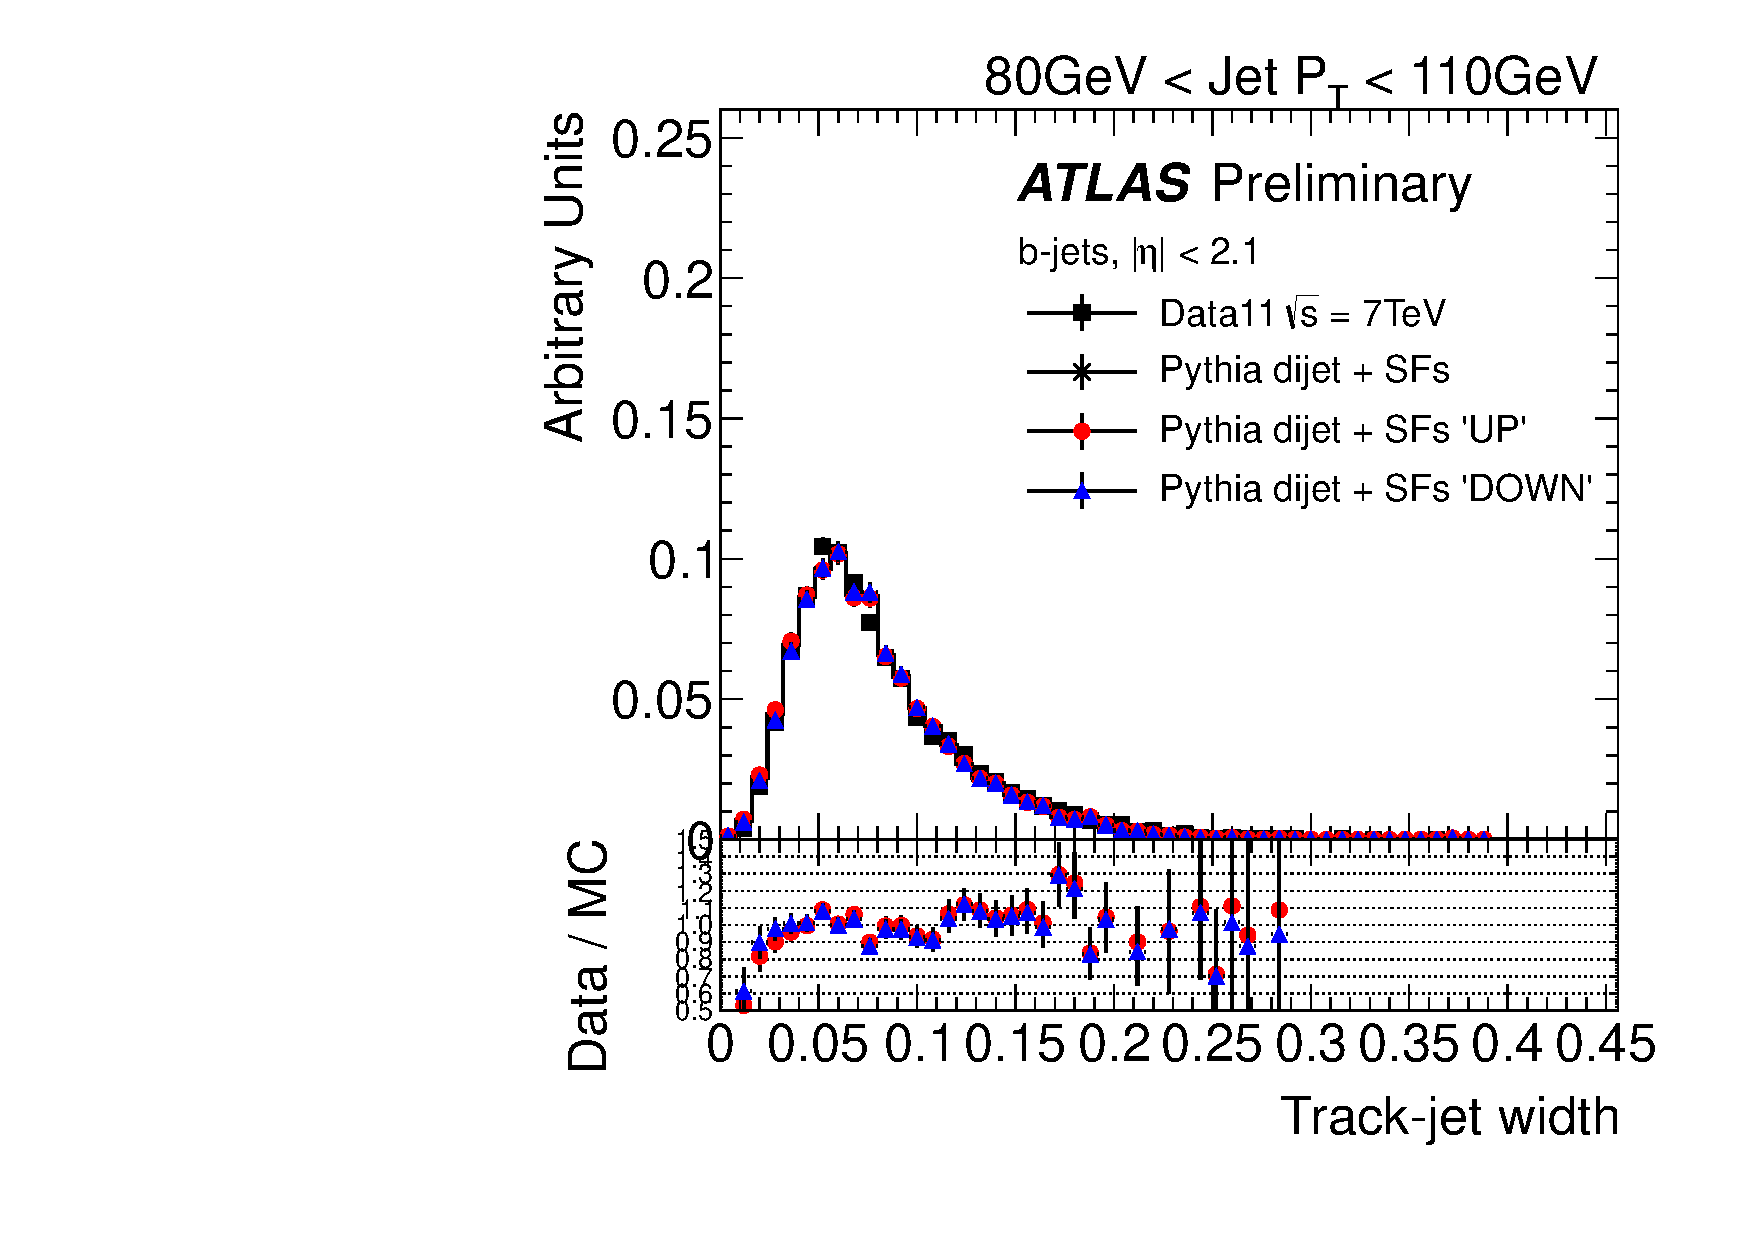
\includegraphics[width=0.49\textwidth]{FIGS/systematics/BTagCalib_DataVarTrkWidthPT080.pdf}
%%%%%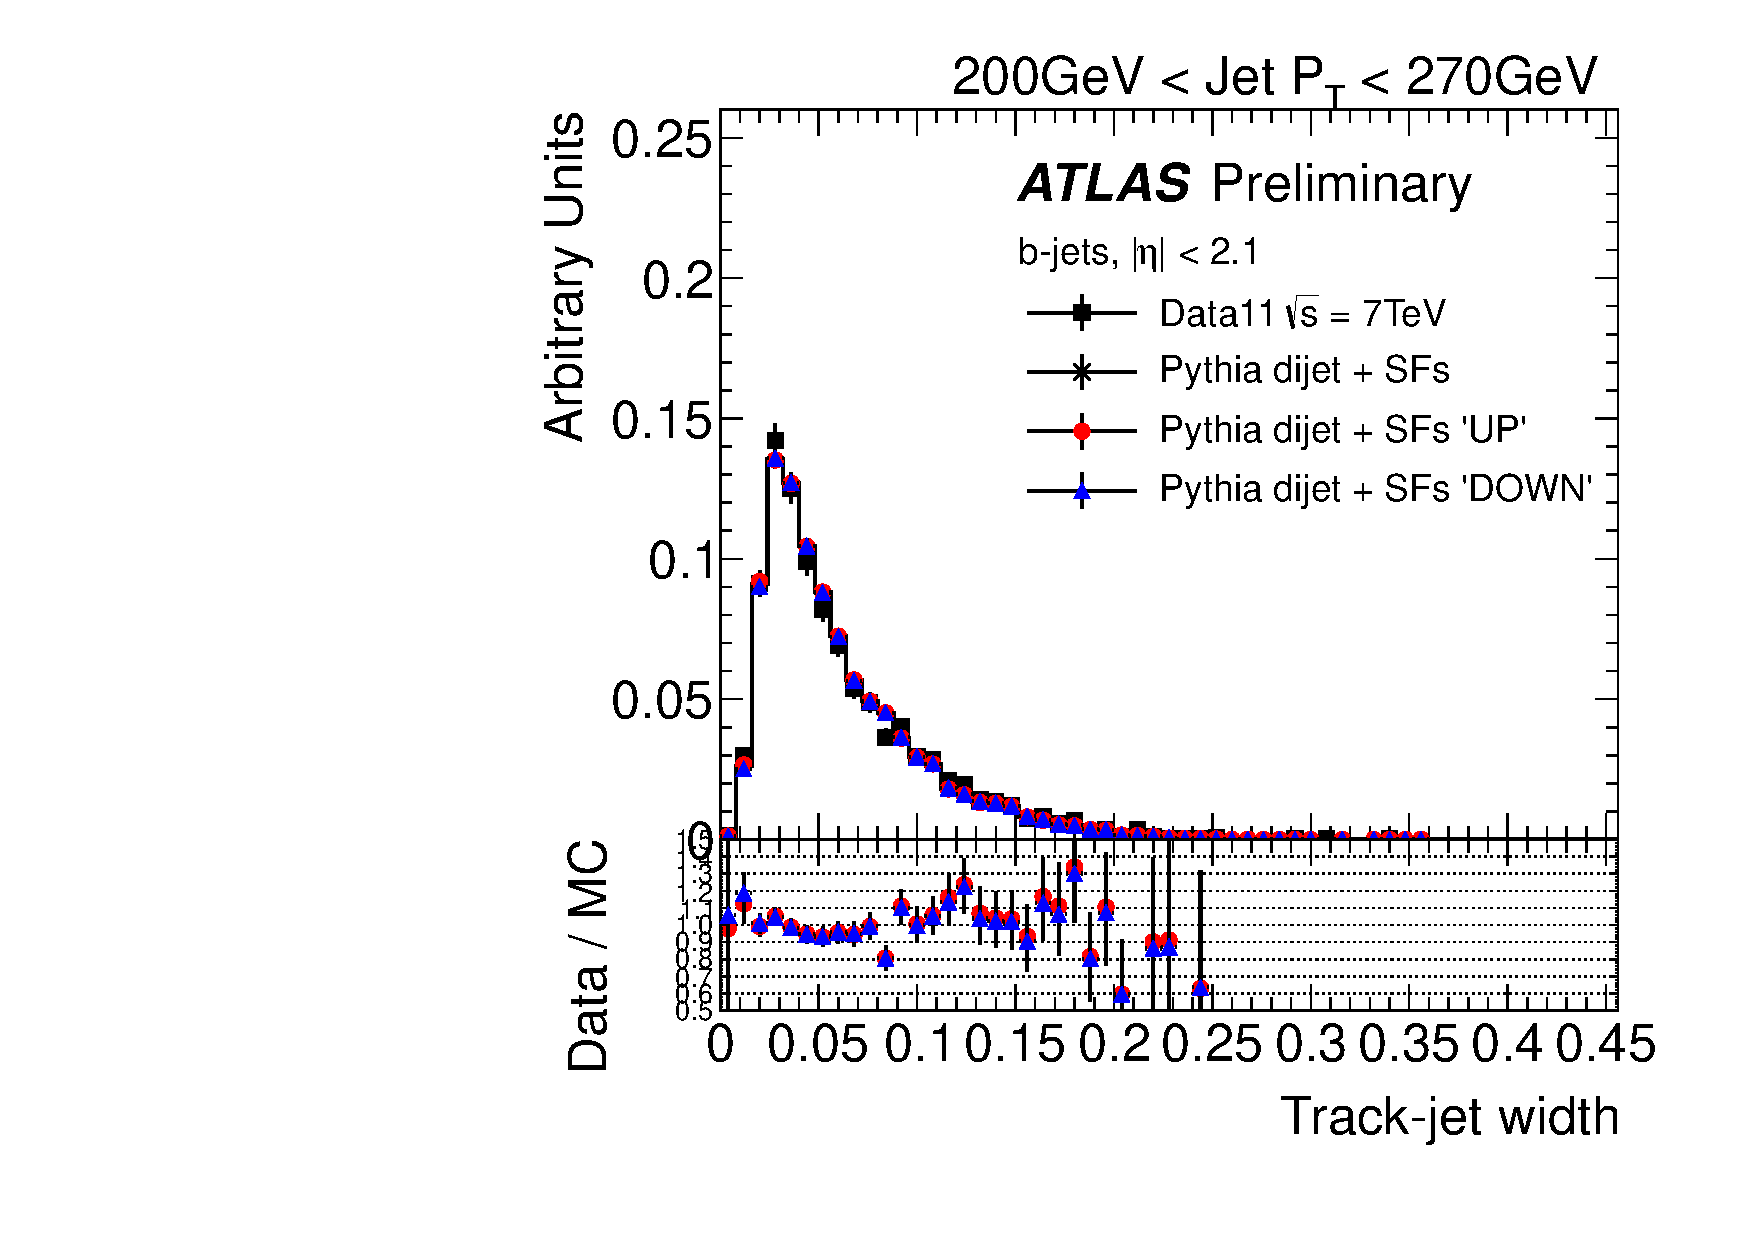
\includegraphics[width=0.49\textwidth]{FIGS/systematics/BTagCalib_DataVarTrkWidthPT200.pdf}
%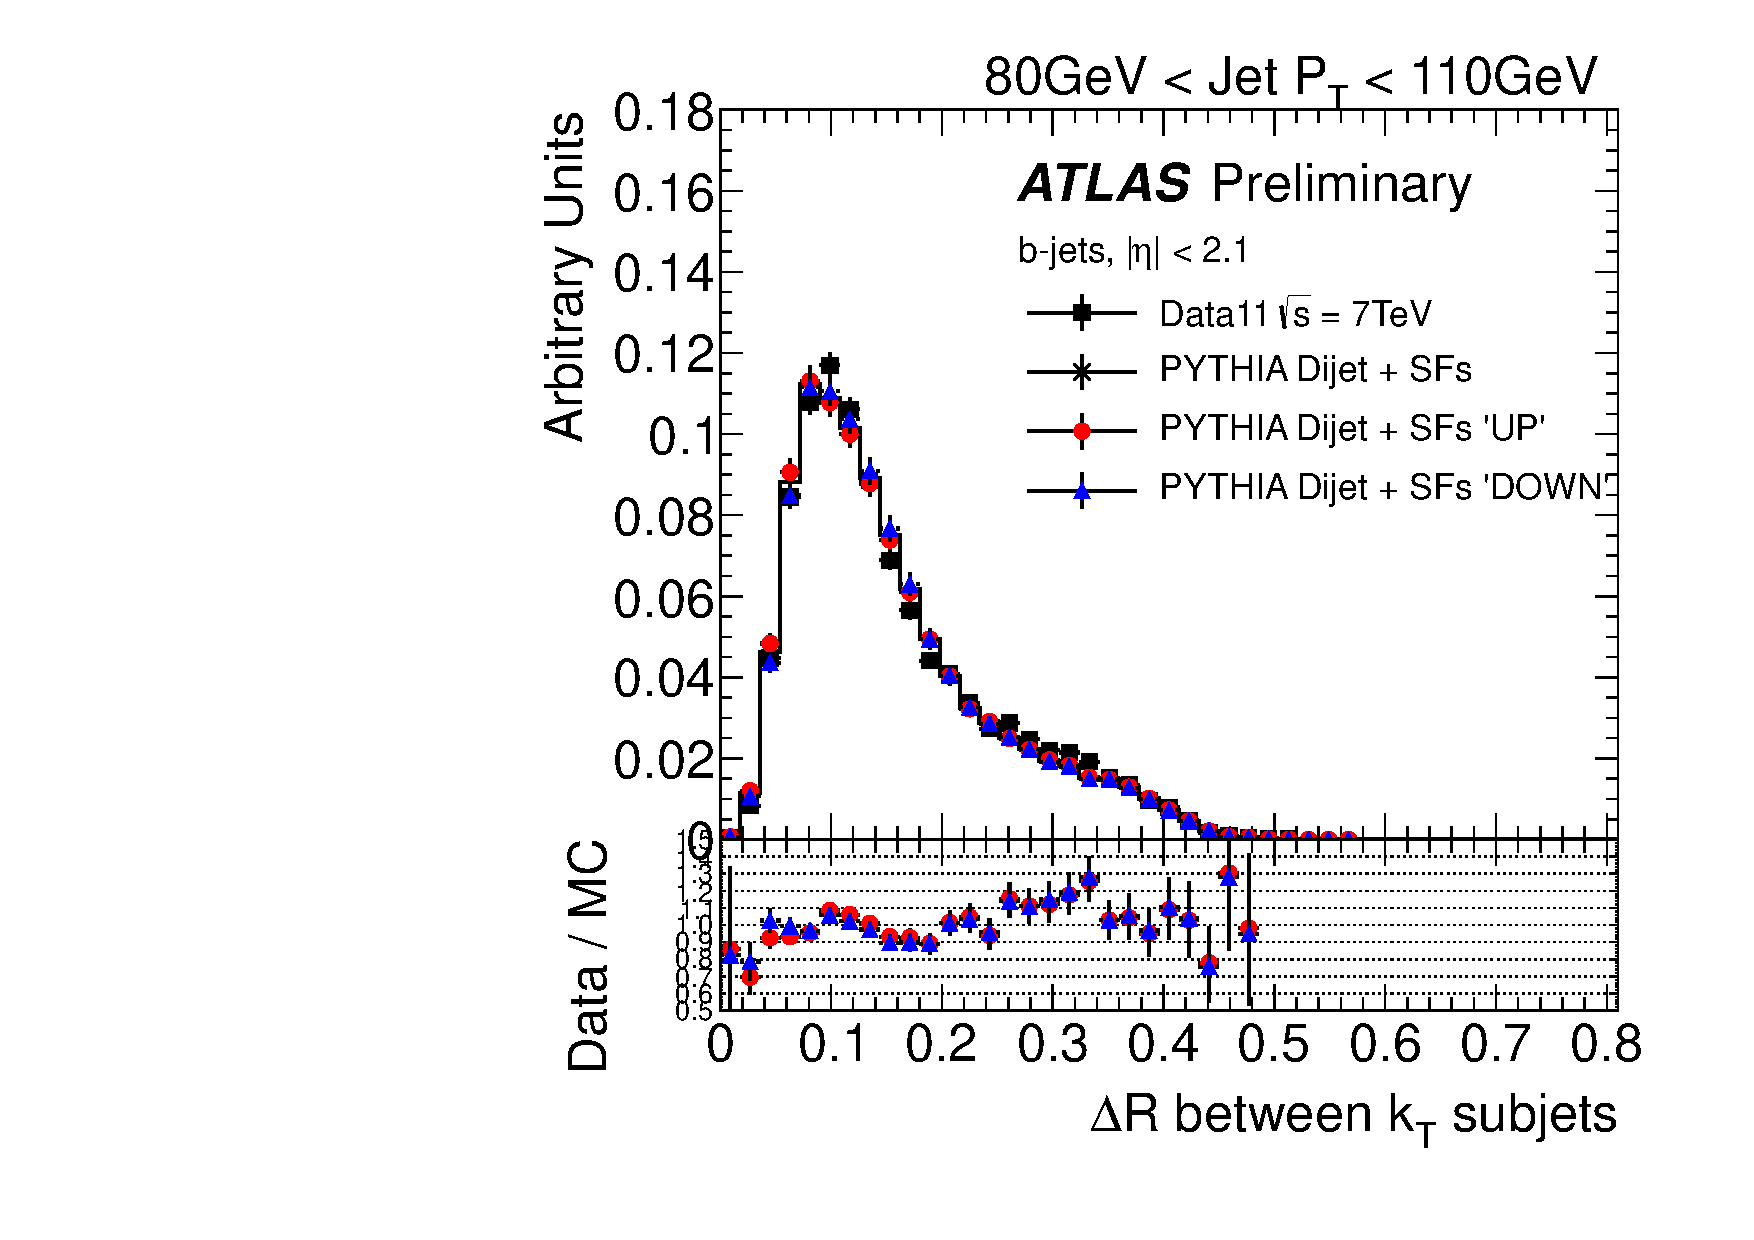
\includegraphics[width=0.49\textwidth]{FIGS/systematics/BTagCalib_DataVarDRktaxisPT080.pdf}
%%%%%%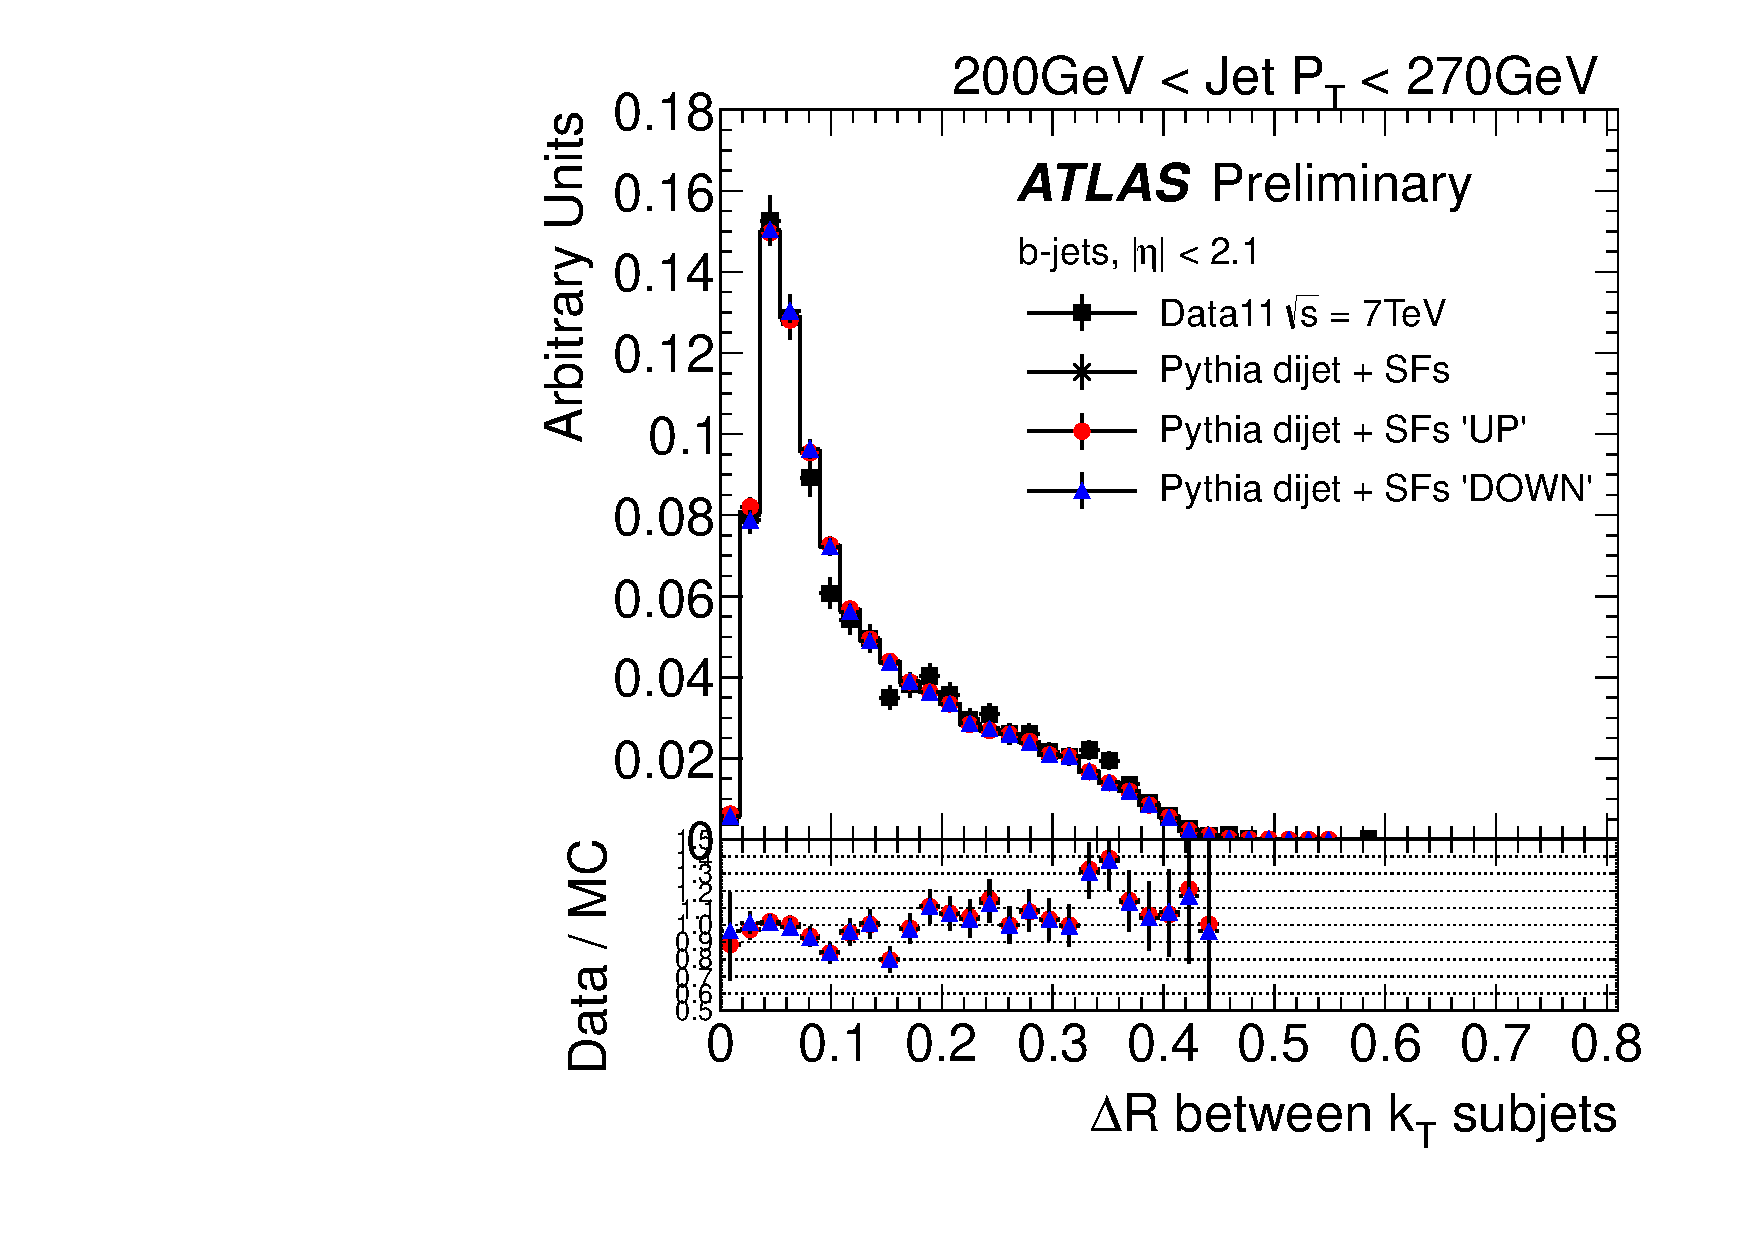
\includegraphics[width=0.49\textwidth]{FIGS/systematics/BTagCalib_DataVarDRktaxisPT200.pdf}
%\caption{The effect of a variation in the $b$-tagging Scale Factors on the tracking variables distributions. Scale Factors were varied up (down) by 1-sigma to evaluate the systematic uncertainty from this source. The ratio data over MC is shown for MC {\sc pythia} with SFs varied up (circles) and down (triangles).}
%\label{fig:btaggingSFs}
%\end{figure}

%\begin{figure}[tp]
%\centering
%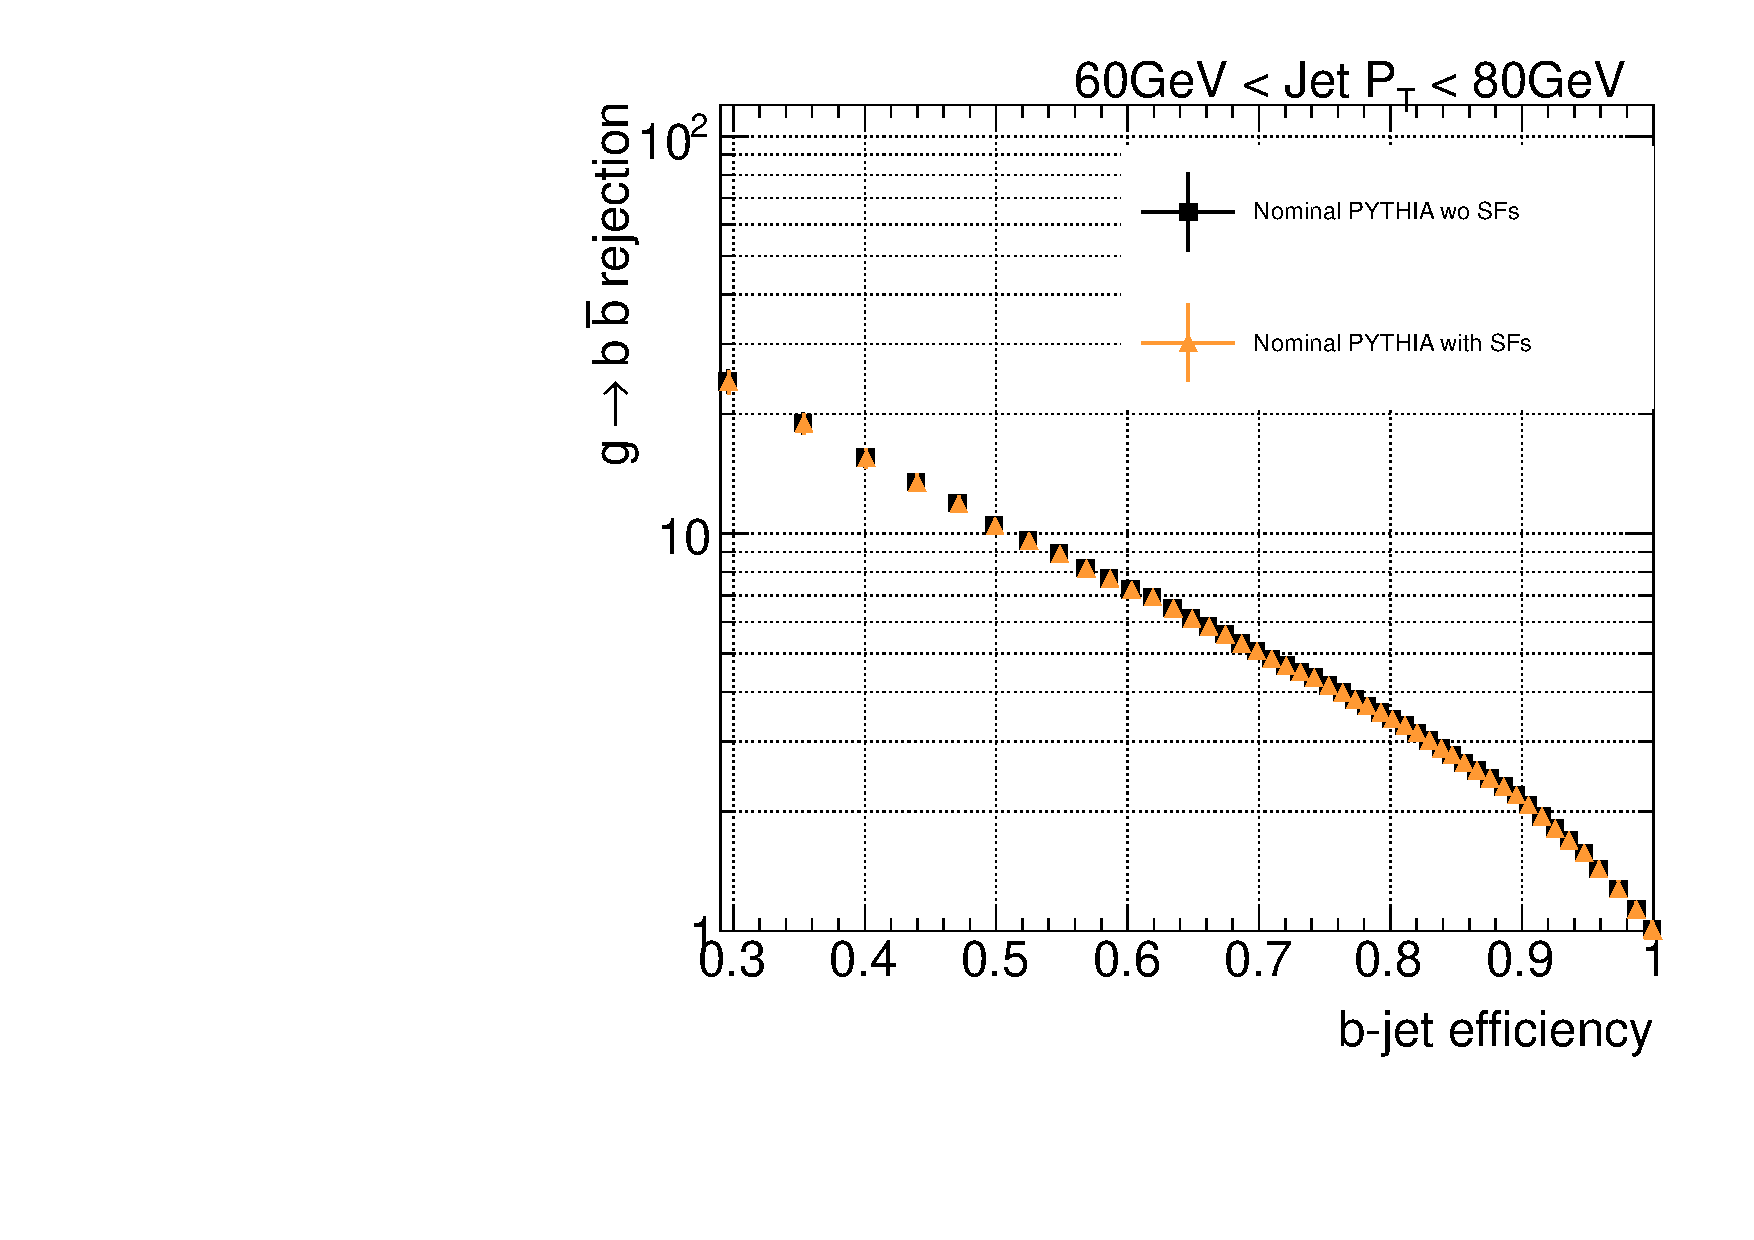
\includegraphics[width=0.49\textwidth]{FIGS/systematics/LlhoodKDE_ISO_BTagCalibTest_rejvseff060.pdf}
%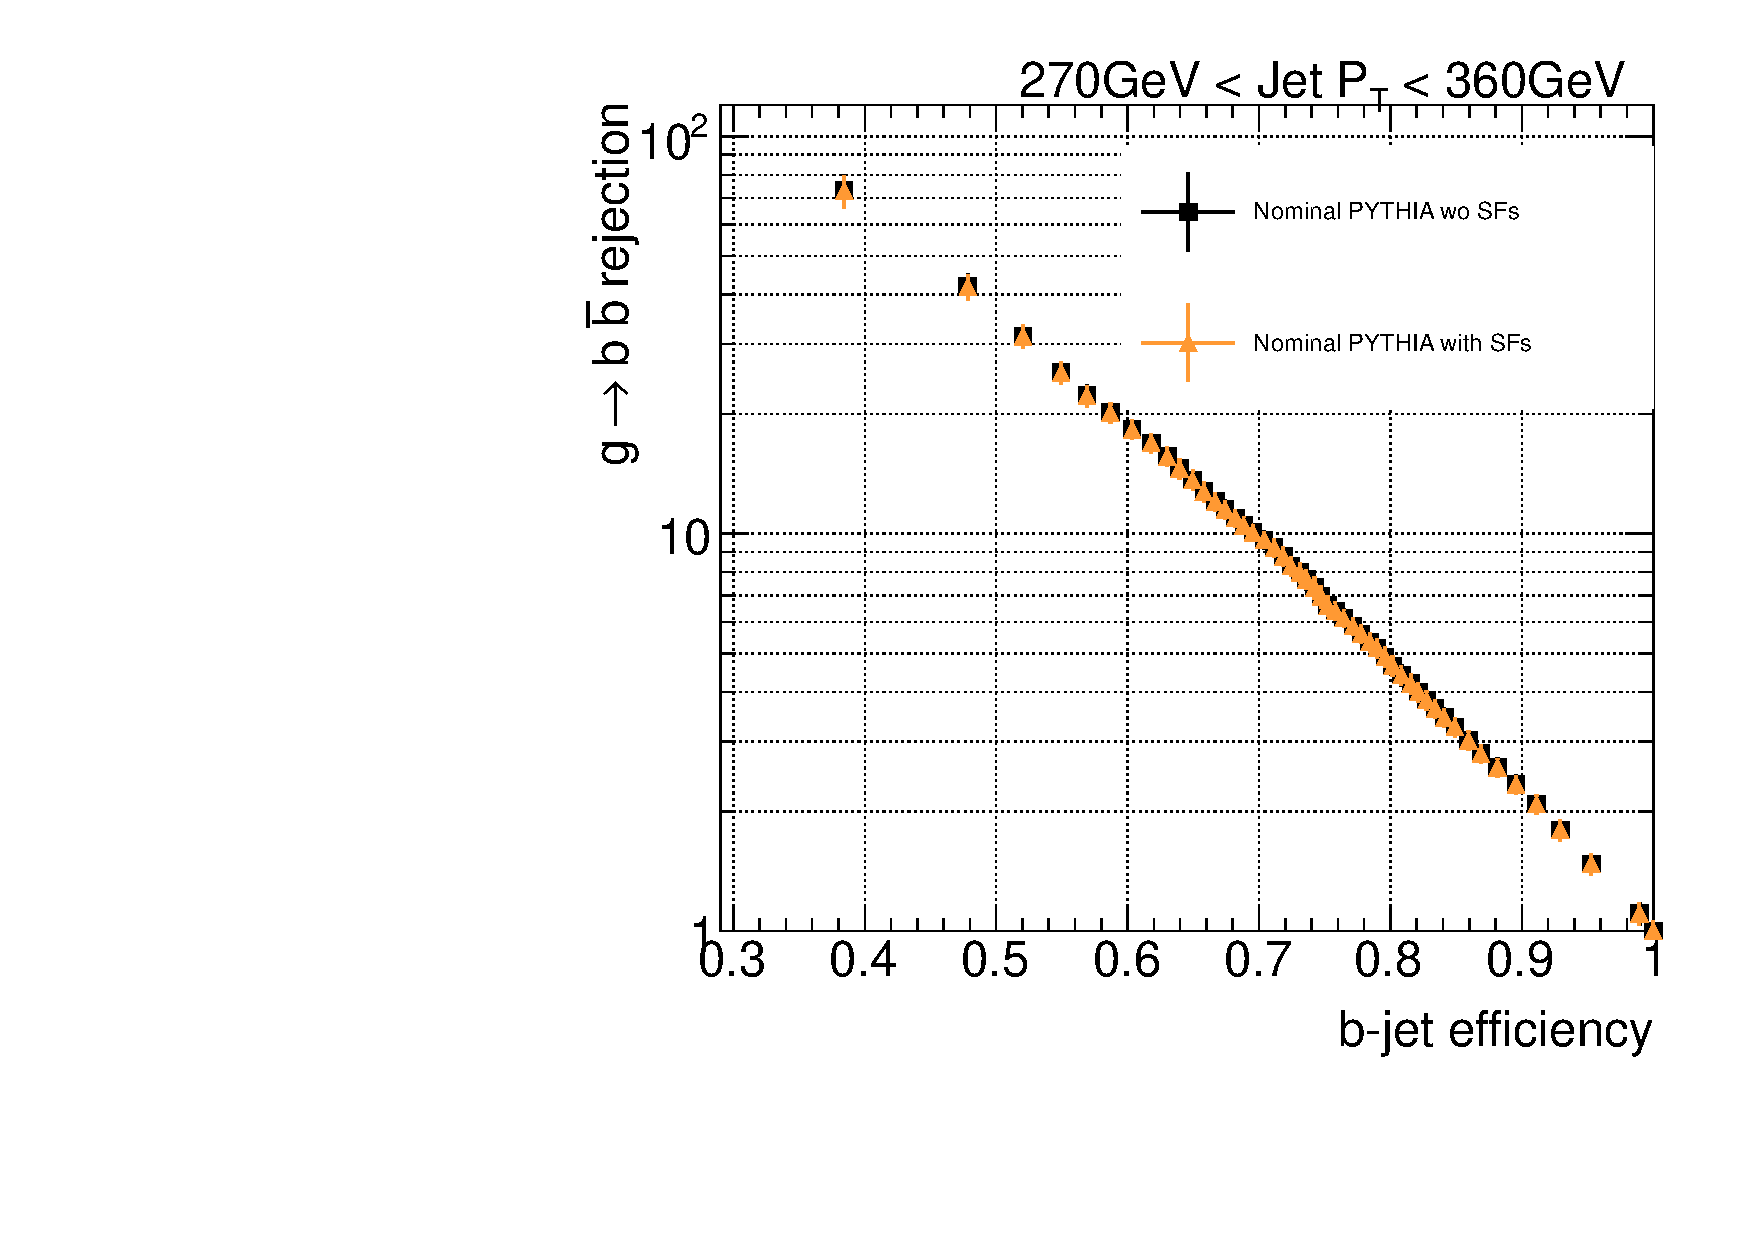
\includegraphics[width=0.49\textwidth]{FIGS/systematics/LlhoodKDE_ISO_BTagCalibTest_rejvseff270.pdf}
%\caption{Rejection of $g\rightarrow b \bar{b}$ merged b-jets as a function of $b$-jet efficiency with and without scale factors.}
%\label{fig:btaggingSFsPerf}
%\end{figure}

%

\vspace{3mm}
{ \em III. Track reconstruction efficiency}
\\[3mm]
This uncertainty arises from the limit in the understanding of the material layout of the Inner Detector. To test its impact a fraction of tracks determined from the track efficiency uncertainty was randomly removed.  % following the method in Ref.~\cite{JetMassNote}.%https://cdsweb.cern.ch/record/1344082?ln=en

The tracking efficiency systematics are given in bins of track $\eta$. For tracks with $p_{\rm{T}}^{\rm{track}} > 500$~MeV the uncertainties are independent of $\pt$:  2\% for $|\eta^{\rm{track}}|<1.3$, 3\% for $1.3<|\eta^{\rm{track}}|<1.9$, 4\% for $1.9<|\eta^{\rm{track}}|<2.1$, 4\% for $2.1<|\eta^{\rm{track}}|<2.3$ and 7\% for $2.3<|\eta^{\rm{track}}|<2.5$~\cite{chargemultiplicity}. All numbers are relative to the corresponding tracking efficiencies.  
%https://cdsweb.cern.ch/record/1286839
%http://arxiv.org/abs/1012.5104

The tracking variables were re-calculated and the performance of the nominal likelihood was evaluated in the new sample with worse tracking efficiency. The rejection-efficiency curves %plots, shown in Fig.~\ref{fig:trackefficiency},
 show a small degradation of the performance which is comparable to the statistical uncertainty. The effect is however systematically present over all 16 \pt\ bin/working points, without a clear \pt\ dependence. We have thus taken the average over \pt, and obtained a global systematic uncertainty of 4\% both for the 50\% and 60\% efficiency working points. The performance comparison is shown in in Fig.~\ref{fig:trackefficiency} for two \pt\ bins. %Similar plots were produced for all other sources of uncertainties considered but are not shown in this note for brevity.

\begin{figure}[tp]
\centering
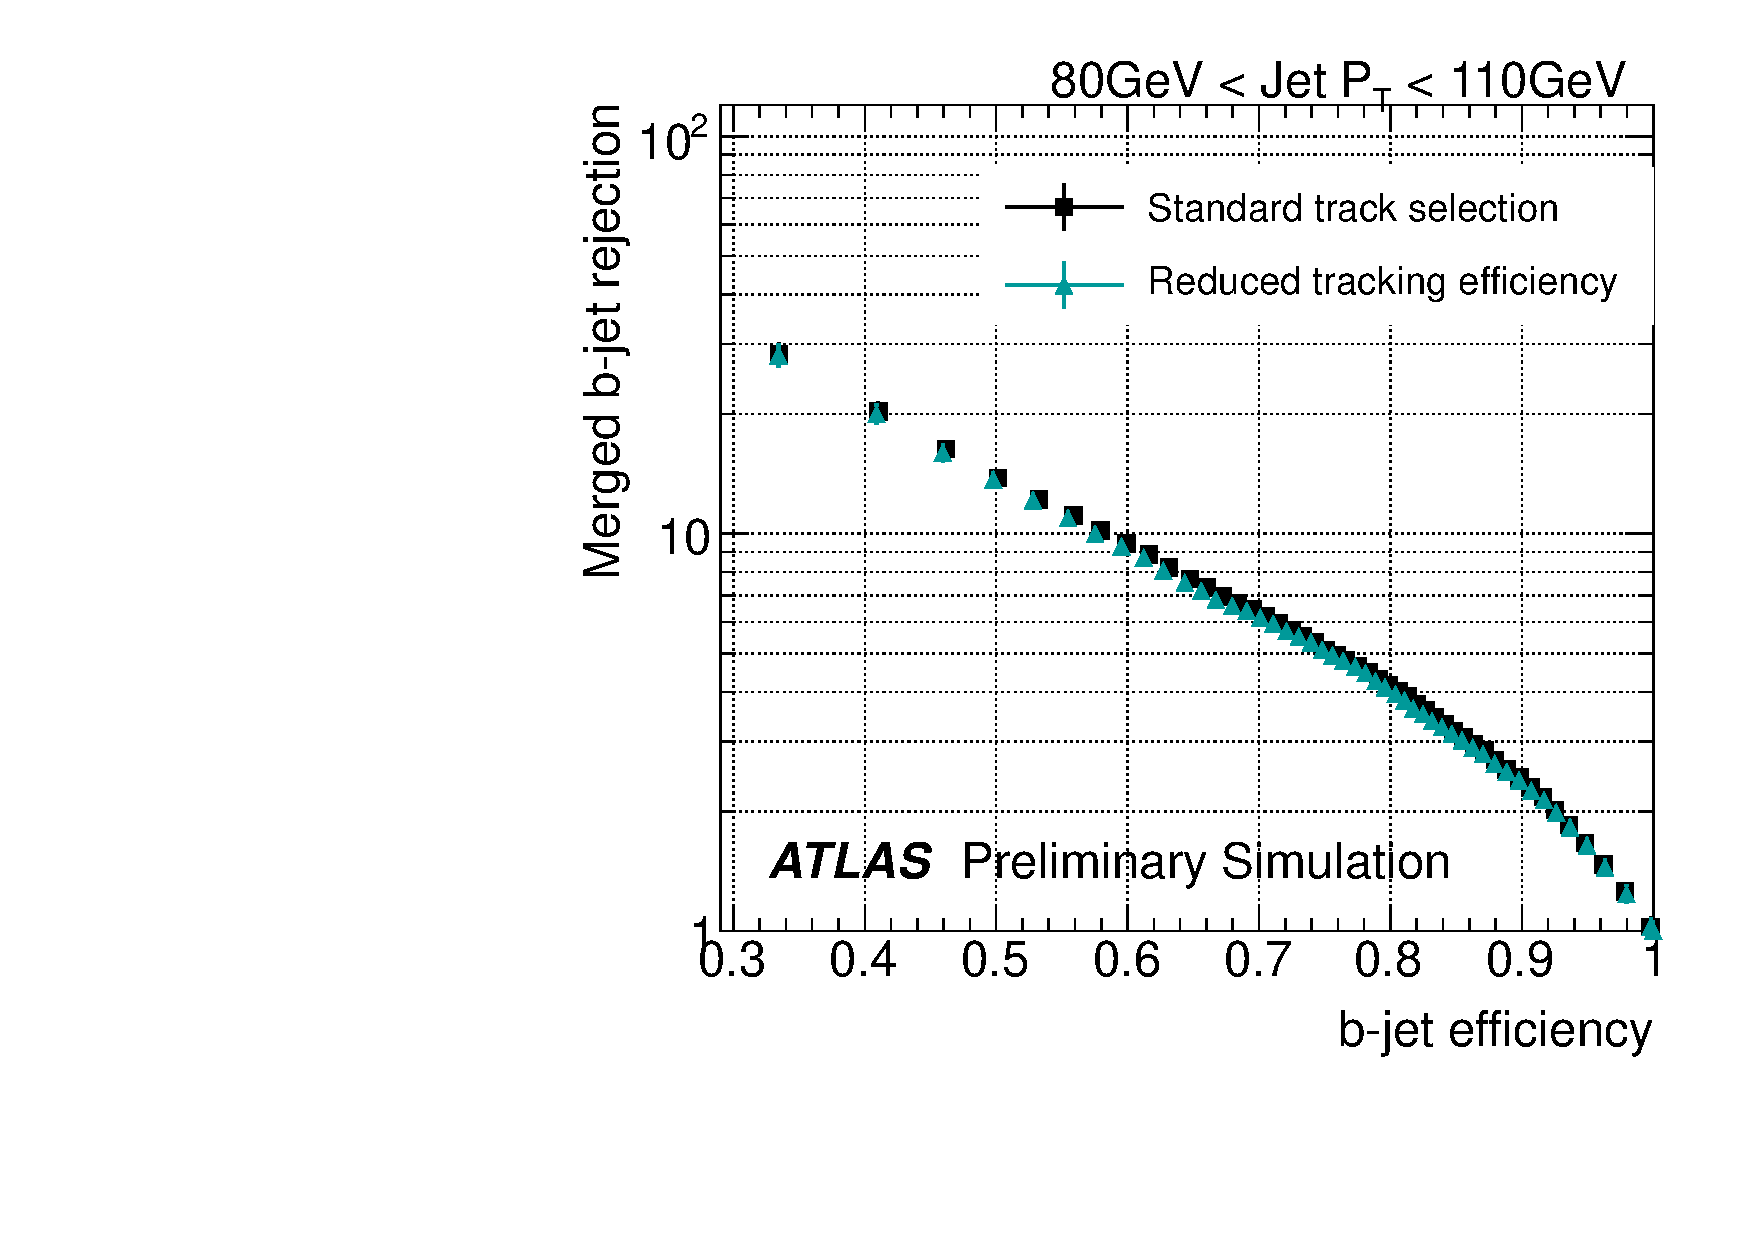
\includegraphics[width=0.49\textwidth]{FIGS/systematics/LlhoodKDE_ISO_TrackingUncertaintyTest_rejvseff080.pdf}
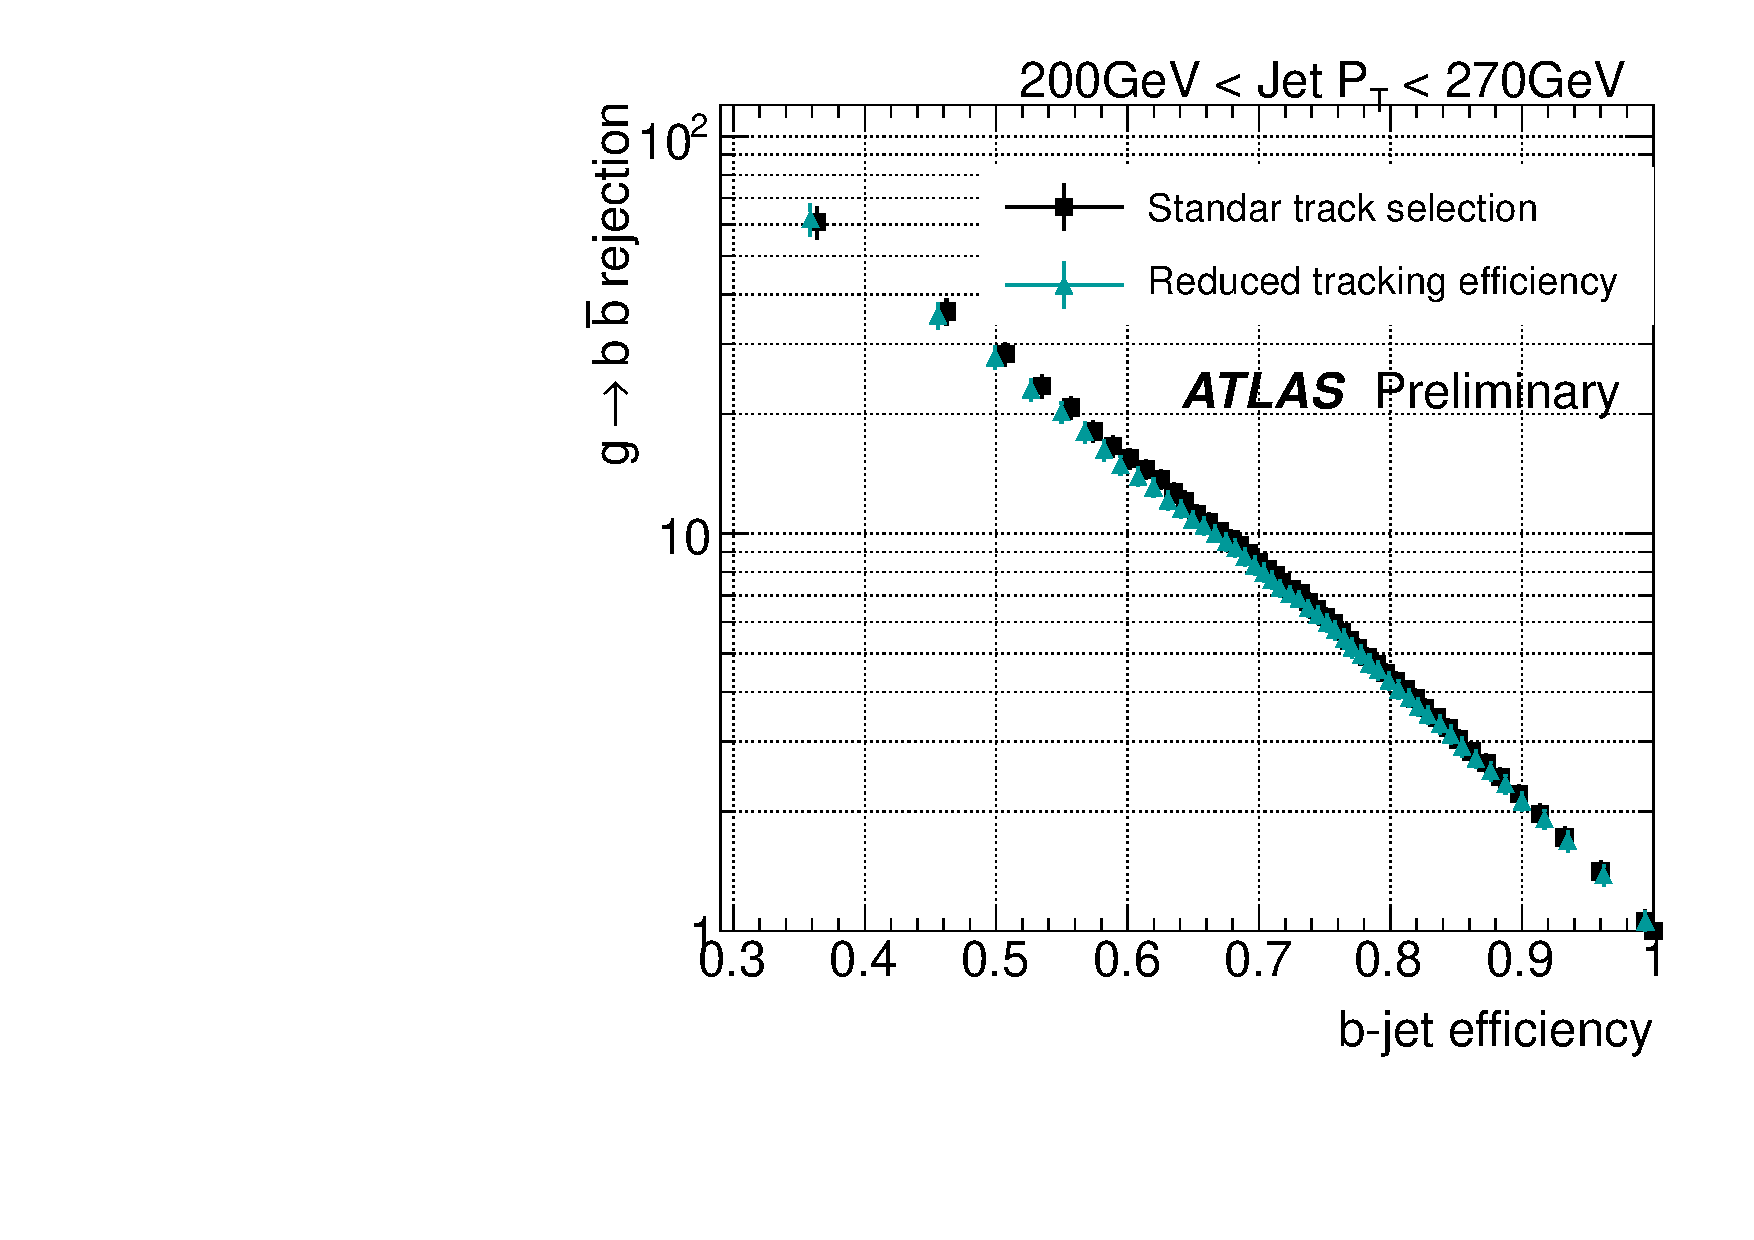
\includegraphics[width=0.49\textwidth]{FIGS/systematics/LlhoodKDE_ISO_TrackingUncertaintyTest_rejvseff200.pdf}
\caption{Rejection of merged $b$-jets as a function of the single $b$-jet efficiency showing shift in likelihood performance caused by a reduction in the tracking efficiency.}
\label{fig:trackefficiency}
\end{figure}

\vspace{3mm}
{\em IV. Track momentum resolution}
\\[3mm]
The knowledge of the track momentum resolution is limited by the precision both in the material description of the Inner Detector and in the mapping of the magnetic field. Its uncertainty propagates to the kinematic variables used in the double $b$-hadron jet tagger. In order to study this effect, track momenta are over-smeared according to the measured resolution uncertainties, before the track selection cuts are applied.  %before computing the rejection. 
The actual smearing is done in 1/\pt, with an upper bound to the resolution uncertainty given by $\sigma(1/\pt)=0.02/\pt$~\cite{ATLAS-CONF-2010-009}. The effect is found to be negligible. %with respect to the statistical uncertainty.

\vspace{3mm}
{ \em V. Jet transverse momentum resolution}
\\[3mm]
The jet momentum resolution was measured for 2011 data and found to be in agreement with the predictions from the {\sc pythia}-based simulation~\cite{JER2011}. The precision of this measurement, determined in $\pt$ and $\eta$ bins,is typically 10\%.
The systematic uncertainty due to the calorimeter jet $\pt$ resolution was estimated by over-smearing the jet $4$-momentum in the simulated data, without changing jet $\eta$ or $\phi$ angles. The performance is found to globally decrease by 6\%, without a particular \pt\ dependence.

%\begin{figure}[tp]
%\centering
%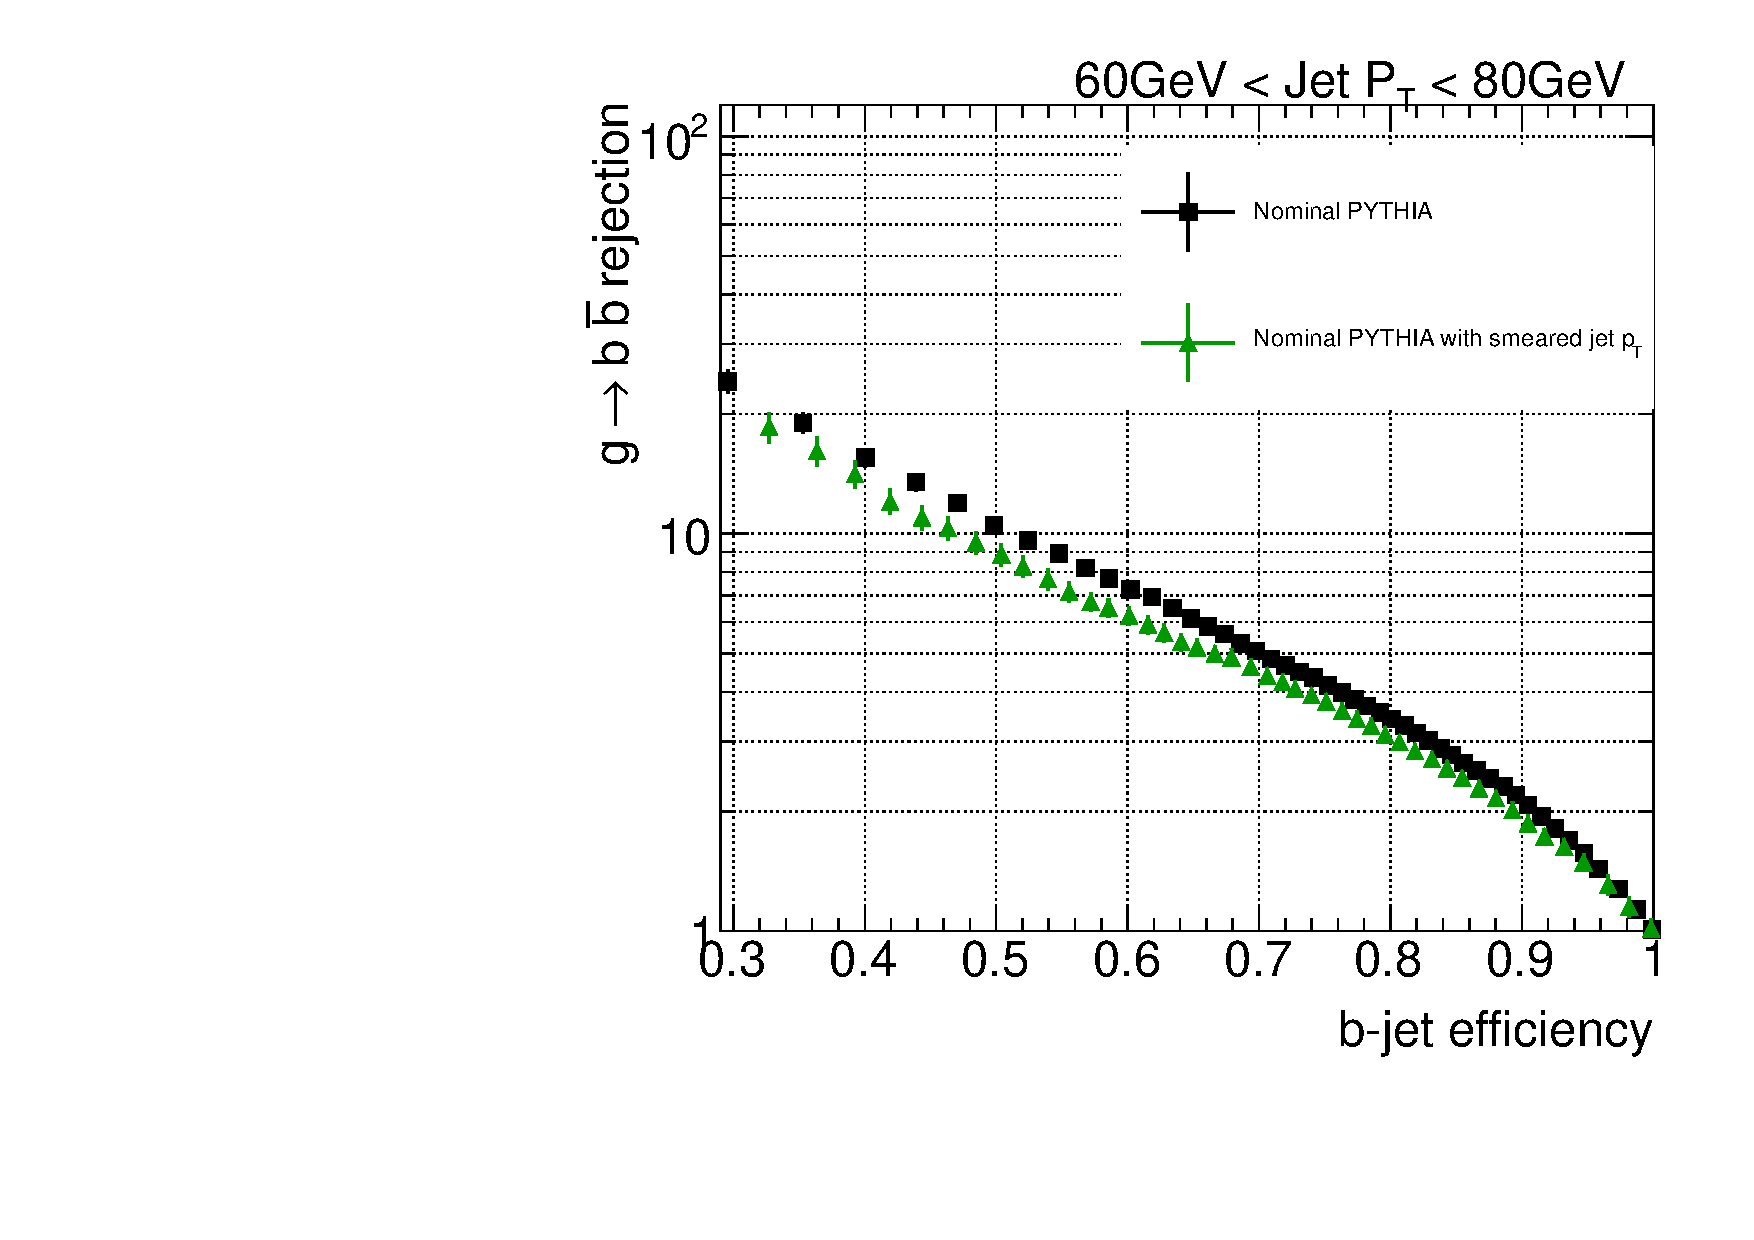
\includegraphics[width=0.49\textwidth]{FIGS/systematics/LlhoodKDE_ISO_SmearedJetPtTest_rejvseff060.pdf}
%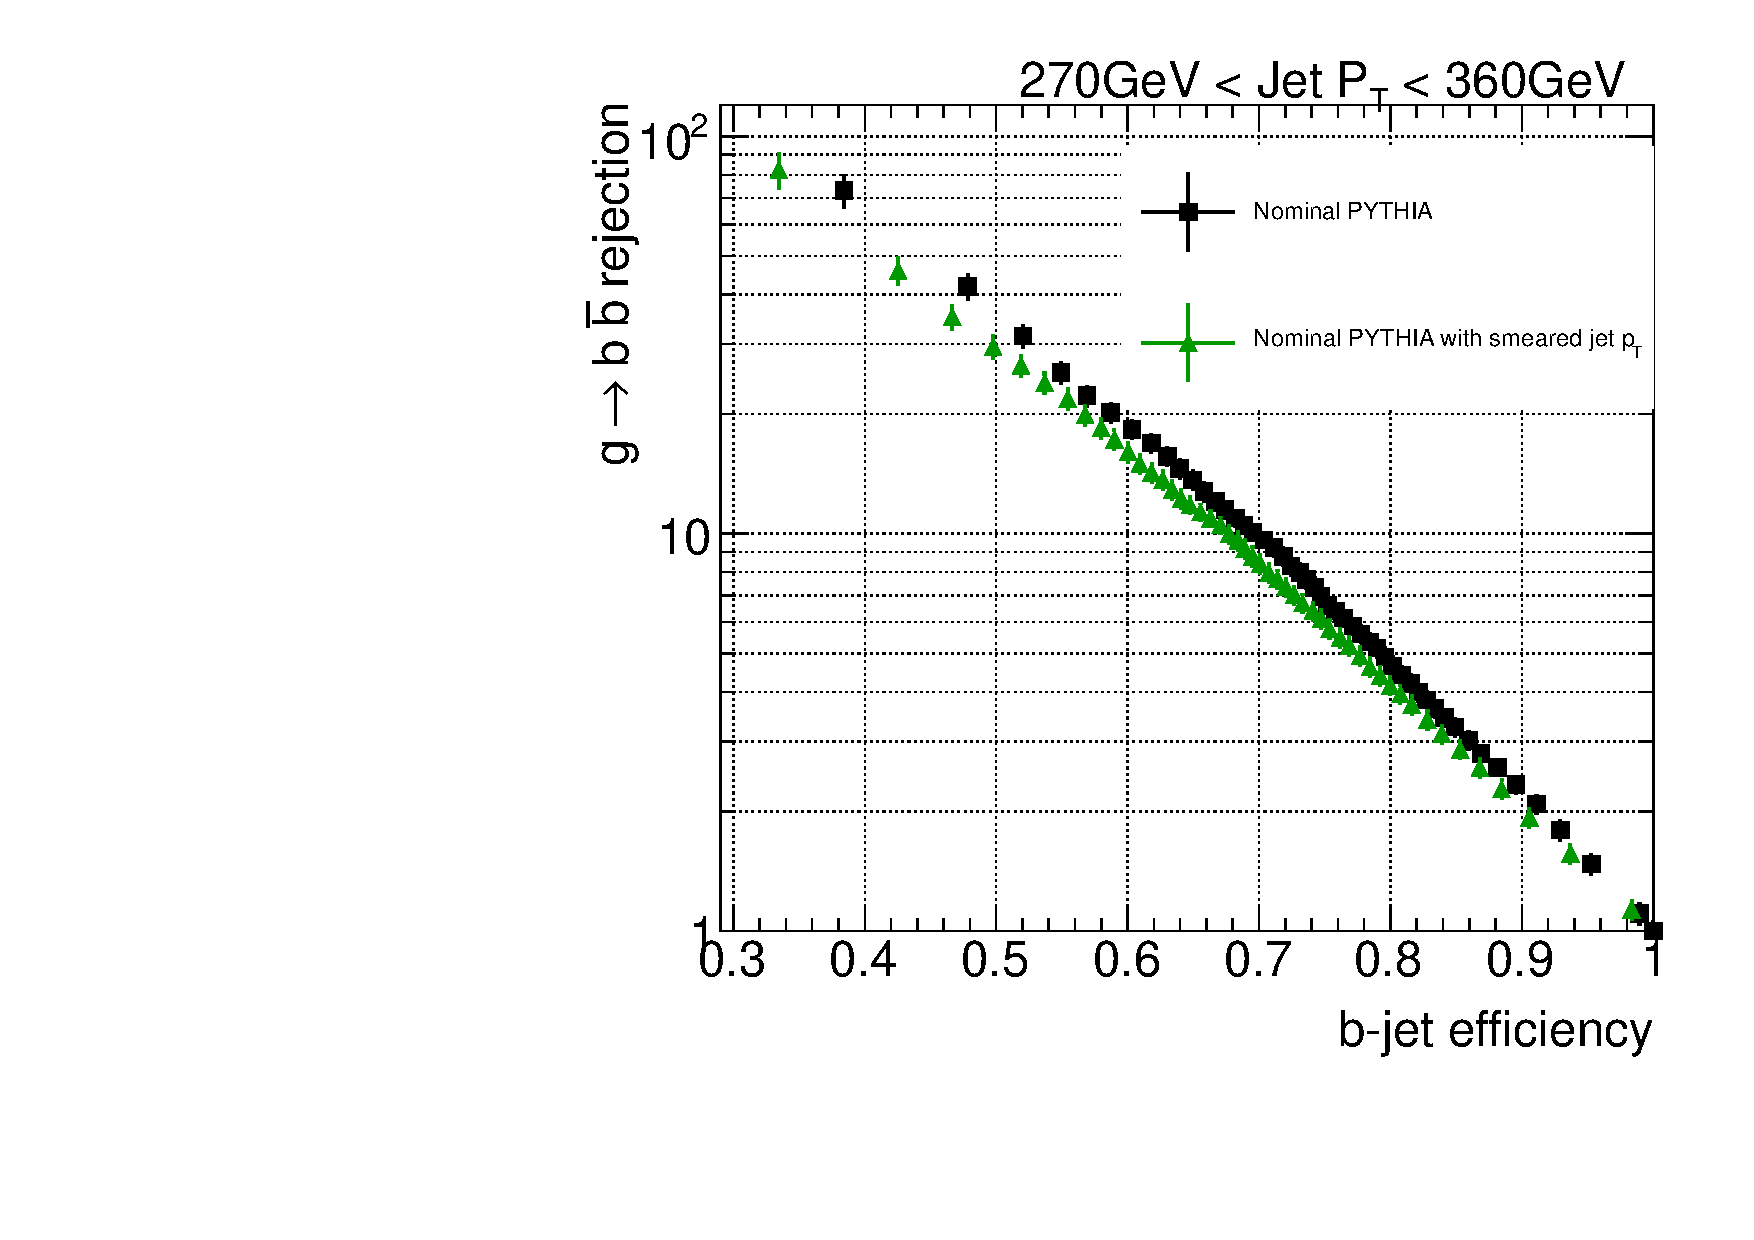
\includegraphics[width=0.49\textwidth]{FIGS/systematics/LlhoodKDE_ISO_SmearedJetPtTest_rejvseff270.pdf}
%\caption{Rejection of $g\rightarrow b \bar{b}$ merged b-jets as a function of $b$-jet efficiency for jets with smeared $\pt$.}
%\label{fig:jetresolution}
%\end{figure}


\vspace{3mm}
{ \em VI. Jet energy scale for heavy flavour jets}
\\[3mm]
%The calorimeter jet response uncertainties for $b$-jets was evaluated using single hadron response measurements in MC samples of inclusive dijet and $b \bar{b}$ dijet events. 
The jet energy scale (JES) uncertainty for light jets reconstructed with the anti-$k_T$ algorithm with distance parameter $R$=0.4 and calibrated to the  EM+JES scale is between $\sim$4\% at low \pt\ and $\sim$2.5\% for jets with  $\pt > $60~GeV in the central region~\cite{bjetJES}. In the case of $b$-jets, and additional uncertainty arising from the modelling of the $b$-quark production mechanism and the $b$-quark fragmentation was determined from systematic variations of the Monte Carlo simulation. % and validated up to $\sim$3\% in 2011 data and MC. 
The resulting fractional additional JES uncertainty for $b$-jets has an upper bound of 2\% for jets with $\pt \leq$100~GeV and it is below 1\% for higher \pt\ jets. To obtain the overall $b$-jet uncertainty this needs to be added in quadrature to the light JES uncertainty. 

The systematic uncertainty originating from the jet energy scale is obtained by scaling the \pt\ of each jet in the simulation up and down by one standard deviation according to the uncertainty of the JES. The effect on the likelihood performance is an average variation of 5\% for the 50\% and 60\% efficiency working points. 


\vspace{3mm}
The different contributions to the systematic uncertainty on the merged $b$-jet rejection are summarized in Table~\ref{tb:systematics}.
\begin{table}[!hbt] %[h]
\renewcommand{\arraystretch}{1.2}
\centering
\begin{tabular}{ | c | c |}
\hline
  ~~~~~~~Systematic source~~~~~~~ &~~Uncertainty~~\\ \hline
  pile-up          &  neglible     \\ 
  $b$-tagging efficiency     &  neglible     \\ 
  track reconstruction efficiency  &    4\%        \\ 
  track \pt\ resolution &  neglible     \\
  jet \pt\ resolution  &    6\%        \\  
  jet energy scale  &    5\%        \\ \hline 
\end{tabular}
\caption{Systematic uncertainities in the merged $b$-jet rejection (common to both the 50\% and the 60\% efficiency working points).}
\label{tb:systematics}
\end{table}

%------------------------------------------------------------------------
\section{Isolation studies}
%------------------------------------------------------------------------
Although the tagger was derived with isolated jets it can also be applied to non-isolated jets. Studies were performed to evaluate the likelihood rejection in $b$-jets with close-by jet with $\pt$ between 7 GeV at electromagnetic scale scale and 90$\%$ of the $b$-jet $\pt$. The results can be seen in  Fig.~\ref{fig:testisolation}. The presence of close-by jets with a susbtancial fraction of the $b$-jet pt worsens the performance in more than 50$\%$ at very high $\pt$. 

\begin{figure}[tp]
\centering
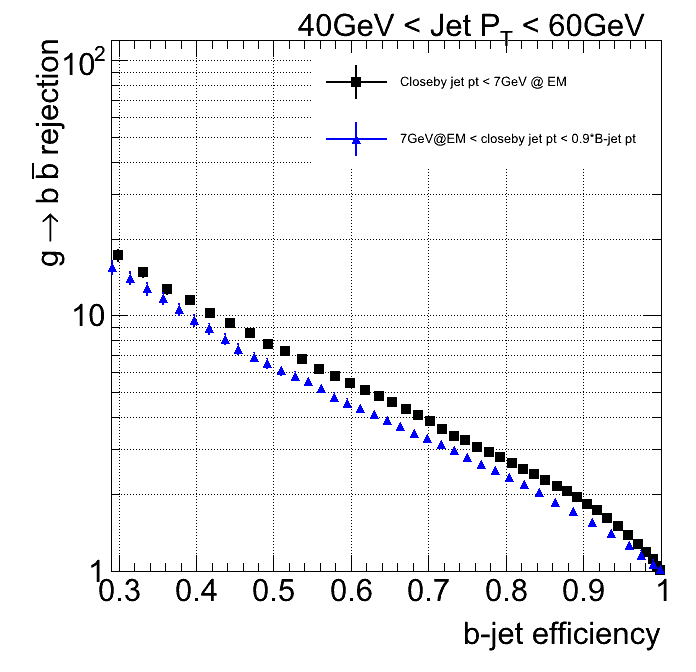
\includegraphics[width=0.4\textwidth]{FIGS/systematics/DiffIsolationCutsKDE_RejvsEff40.png}
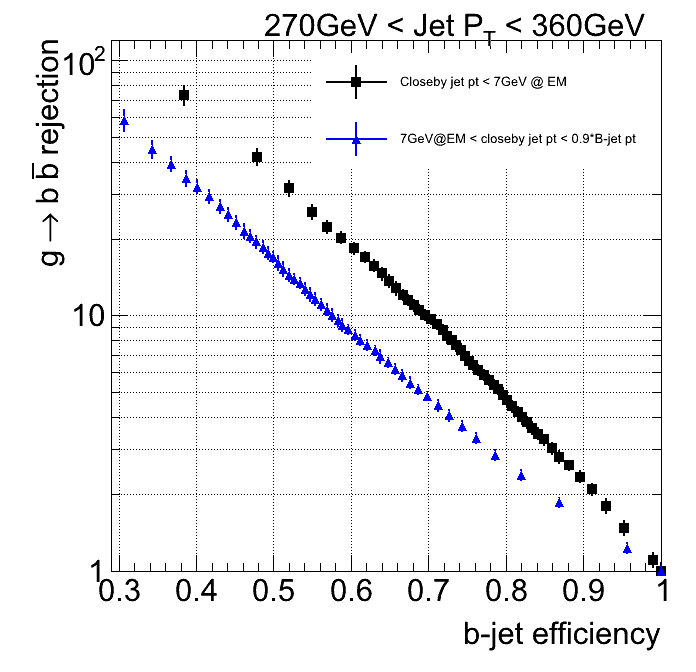
\includegraphics[width=0.4\textwidth]{FIGS/systematics/DiffIsolationCutsKDE_RejvsEff270.png}
\caption{Rejection of $g\rightarrow b \bar{b}$ merged b-jets as a function of $b$-jet efficiency for two different isolation cuts.}
\label{fig:testisolation}
\end{figure}


%------------------------------------------------------------------------
\section{Other Monte Carlo generators}\label{sec:otherMC}
%------------------------------------------------------------------------
%{\em Uncertainties due to the event modelling in the Monte Carlo generators}

The development, training and performance determination of the tagger has been done using Monte Carlo events generated with the {\sc pythia} event simulator, interfaced to the {\sc geant4} based simulation of the ATLAS detector. An immediate question is what the performance would be if studied with a different simulation. In this section we investigate this question for the Perugia tune of {\sc pythia8} and the {\sc herwig++} event generators.

Fig.~\ref{fig:performanceotherMC} shows a comparison of the likelihood rejection, at the 50\% efficiency working point,  between nominal {\sc pythia} and the alternative simulations % for four selected $\pt$ bins covering the full kinematic range. 
as a function of the jet $\pt$ . The larger errors are due to the reduced statistics available, which are even lower for the Perugia case than for {\sc herwig}.



%In order to account for the dependence on different generator models and tunes the likelihood performance was tested using other Monte Carlo simulations. Results with nominal Pythia were compared to the performance derived with dijet samples generated with Herwig++ and with the Perugia tune of Pythia. The comparison can be seen in Fig.~\ref{fig:performanceotherMC}. 

The performance in {\sc herwig} shows a systematic trend, with agreement at low $\pt$ and increasingly poor performances compared to {\sc pythia} as $\pt$ grows. For the Perugia tune, on the other hand, there is no definite behavior, with the performance fluctuating above or below the nominal simulation for different $\pt$ bins consistently with the statistical uncertainties.

The reason for the systematic difference observed between the performances of {\sc pythia} and {\sc herwig} can be traced to the extent with which jets are accurately modelled. Fig.~\ref{fig:herwigdatamc} compares the measured jet track multiplicity distributions in $b$-tagged jets and the prediction from both simulations, for low and high $\pt$ jets. It is observed that indeed {\sc herwig++} does not correctly reproduce the data, particularly at high $\pt$. The level of agreement is found to be better for track-jet width and the $\Delta R$ between the axes of the two $k_t$ subjets in the jet, the two other variables used for discrimination.



%the comparion between jet distribution in experimental data and  Herwig++ Monte Carlo events was performed for $b$-tagged jets. The results for the jet track-multiplicity can be seen in Fig.~\ref{fig:herwigdatamc}. We find that Herwig++ does not reproduce data jet distributions correctly at medium and high \pt.



\begin{figure}[tp]
\centering
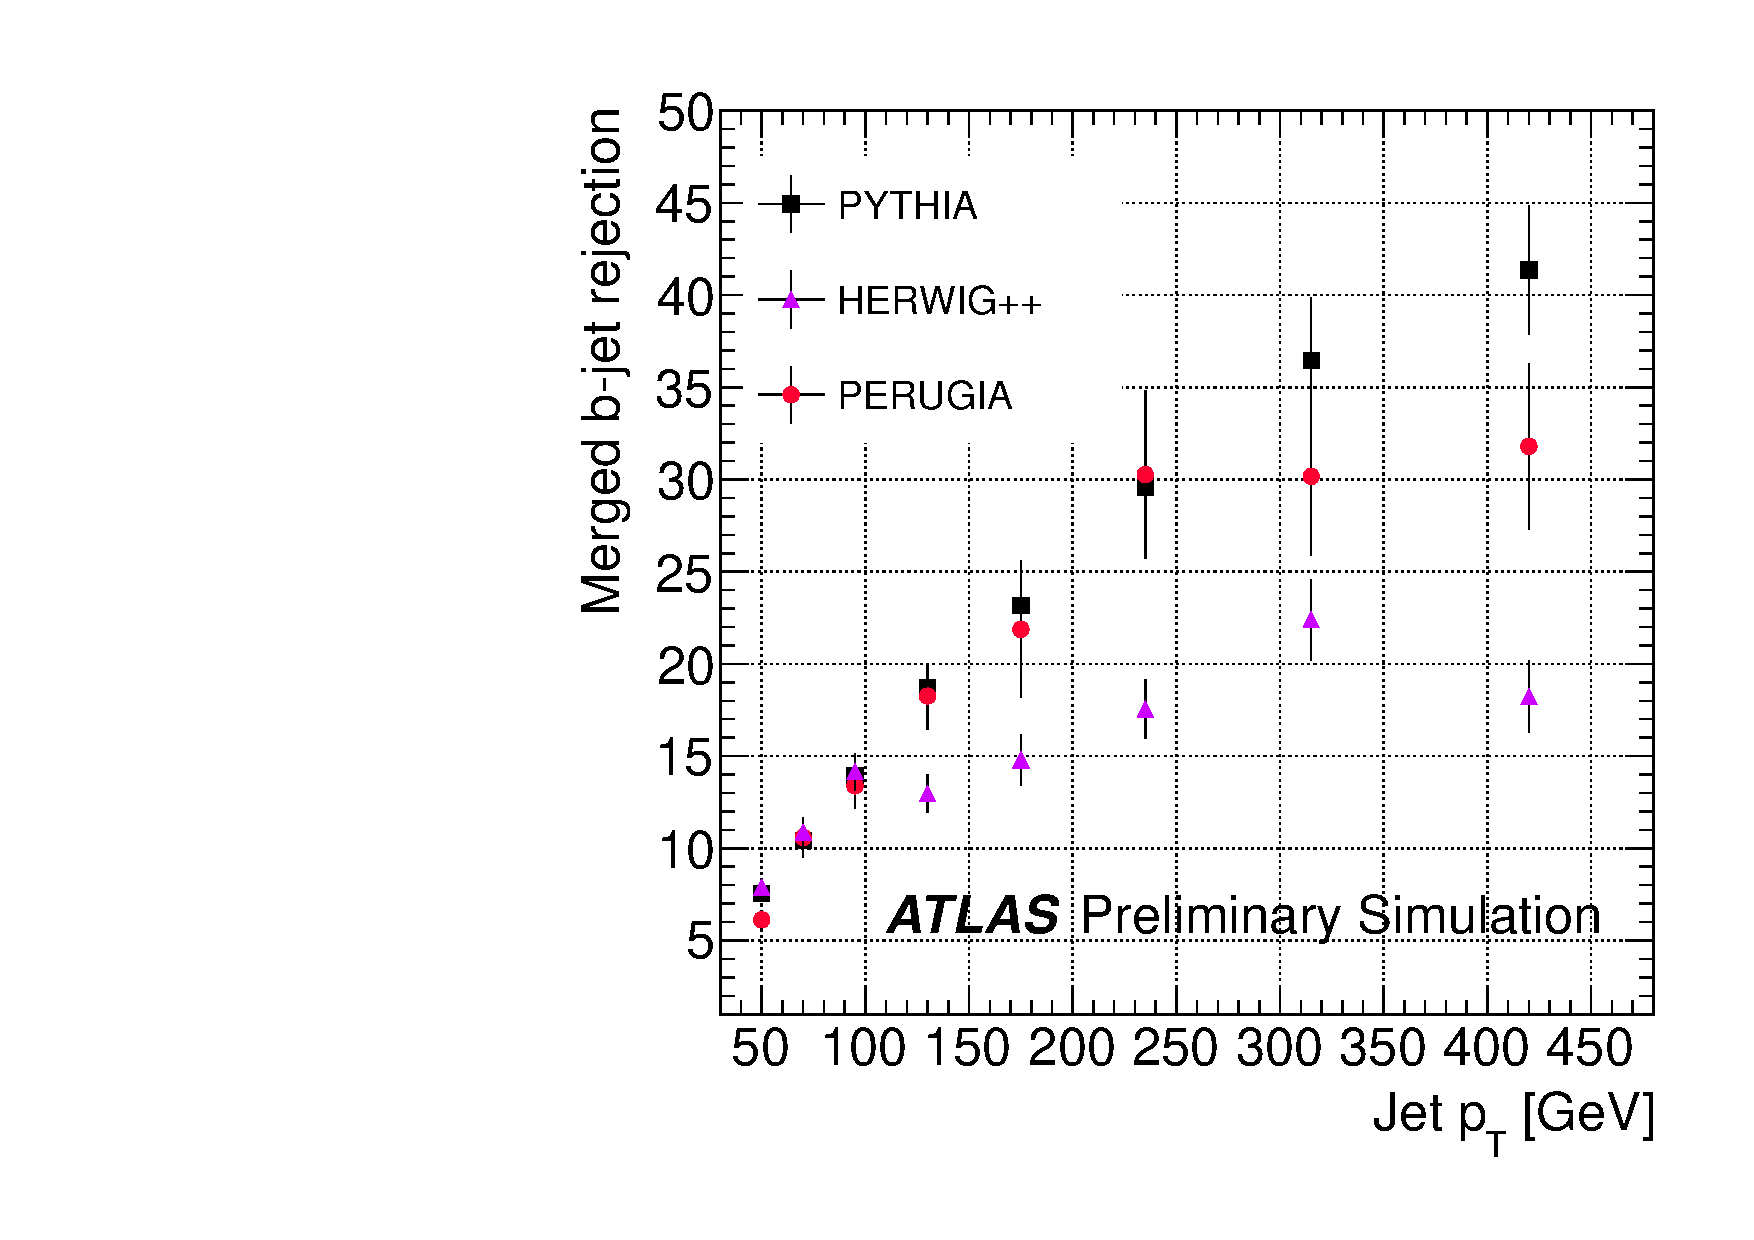
\includegraphics[width=0.49\textwidth]{gbbRejection_vs_PT_3MonteCarlos_50Eff.pdf}
%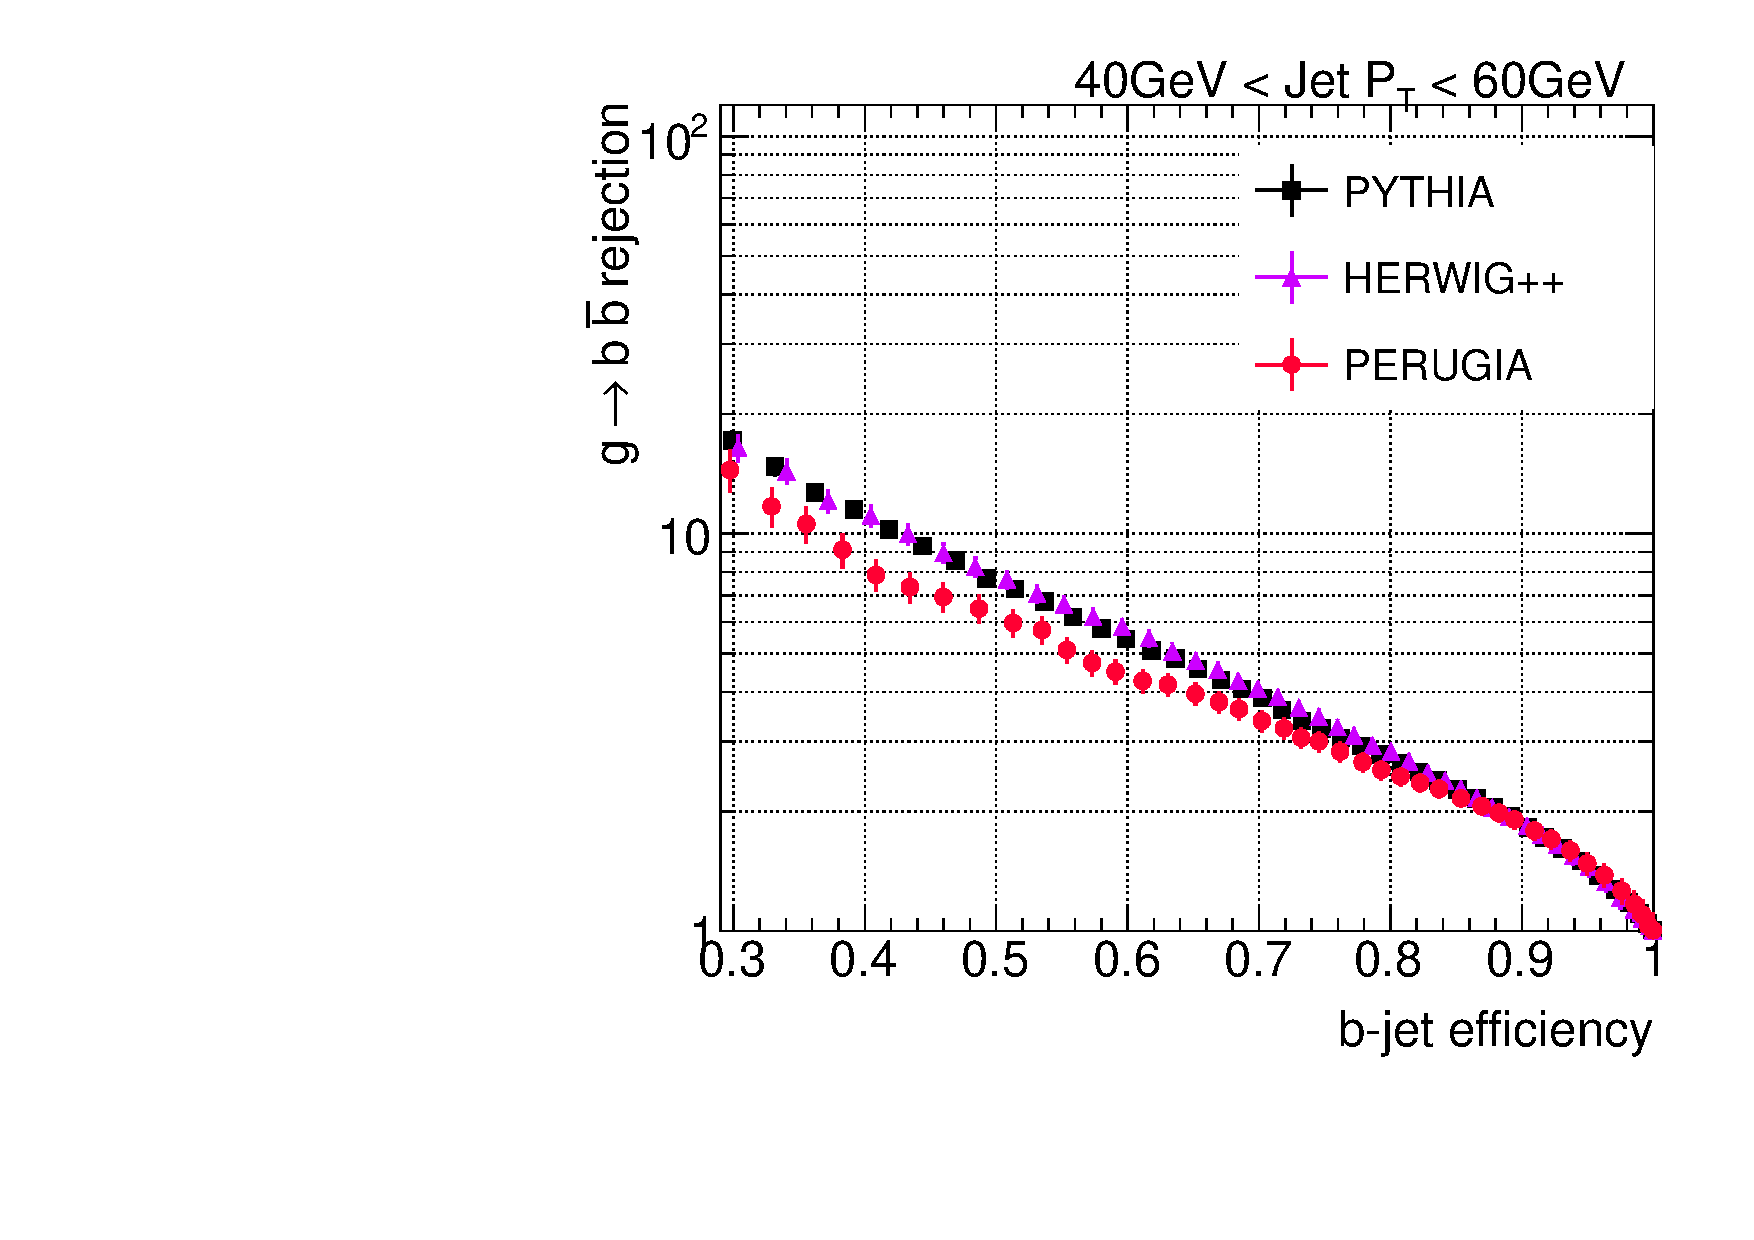
\includegraphics[width=0.49\textwidth]{FIGS/systematics/newInterpLlhoodKDE_ISO_DiffMCGen_rejvseff040.pdf}
%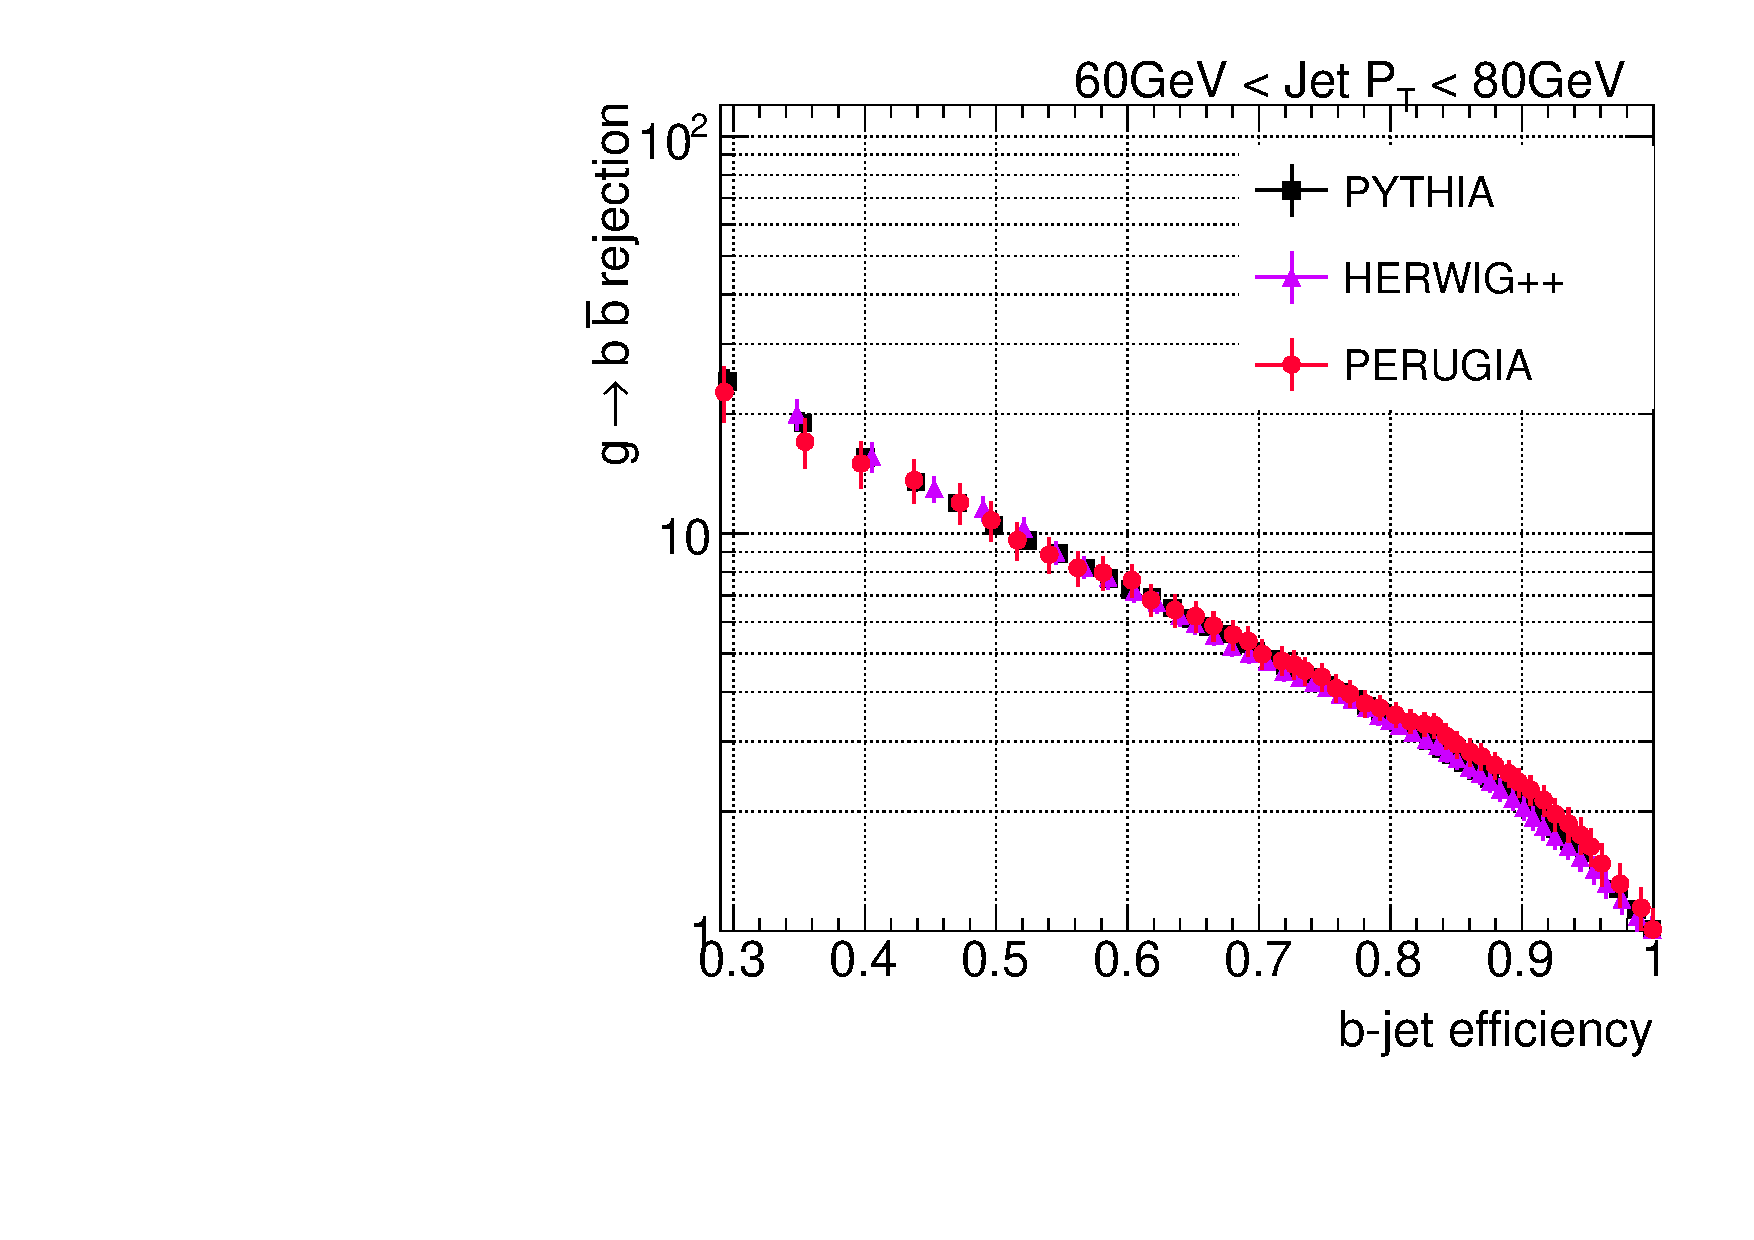
\includegraphics[width=0.49\textwidth]{FIGS/systematics/newInterpLlhoodKDE_ISO_DiffMCGen_rejvseff060.pdf}
%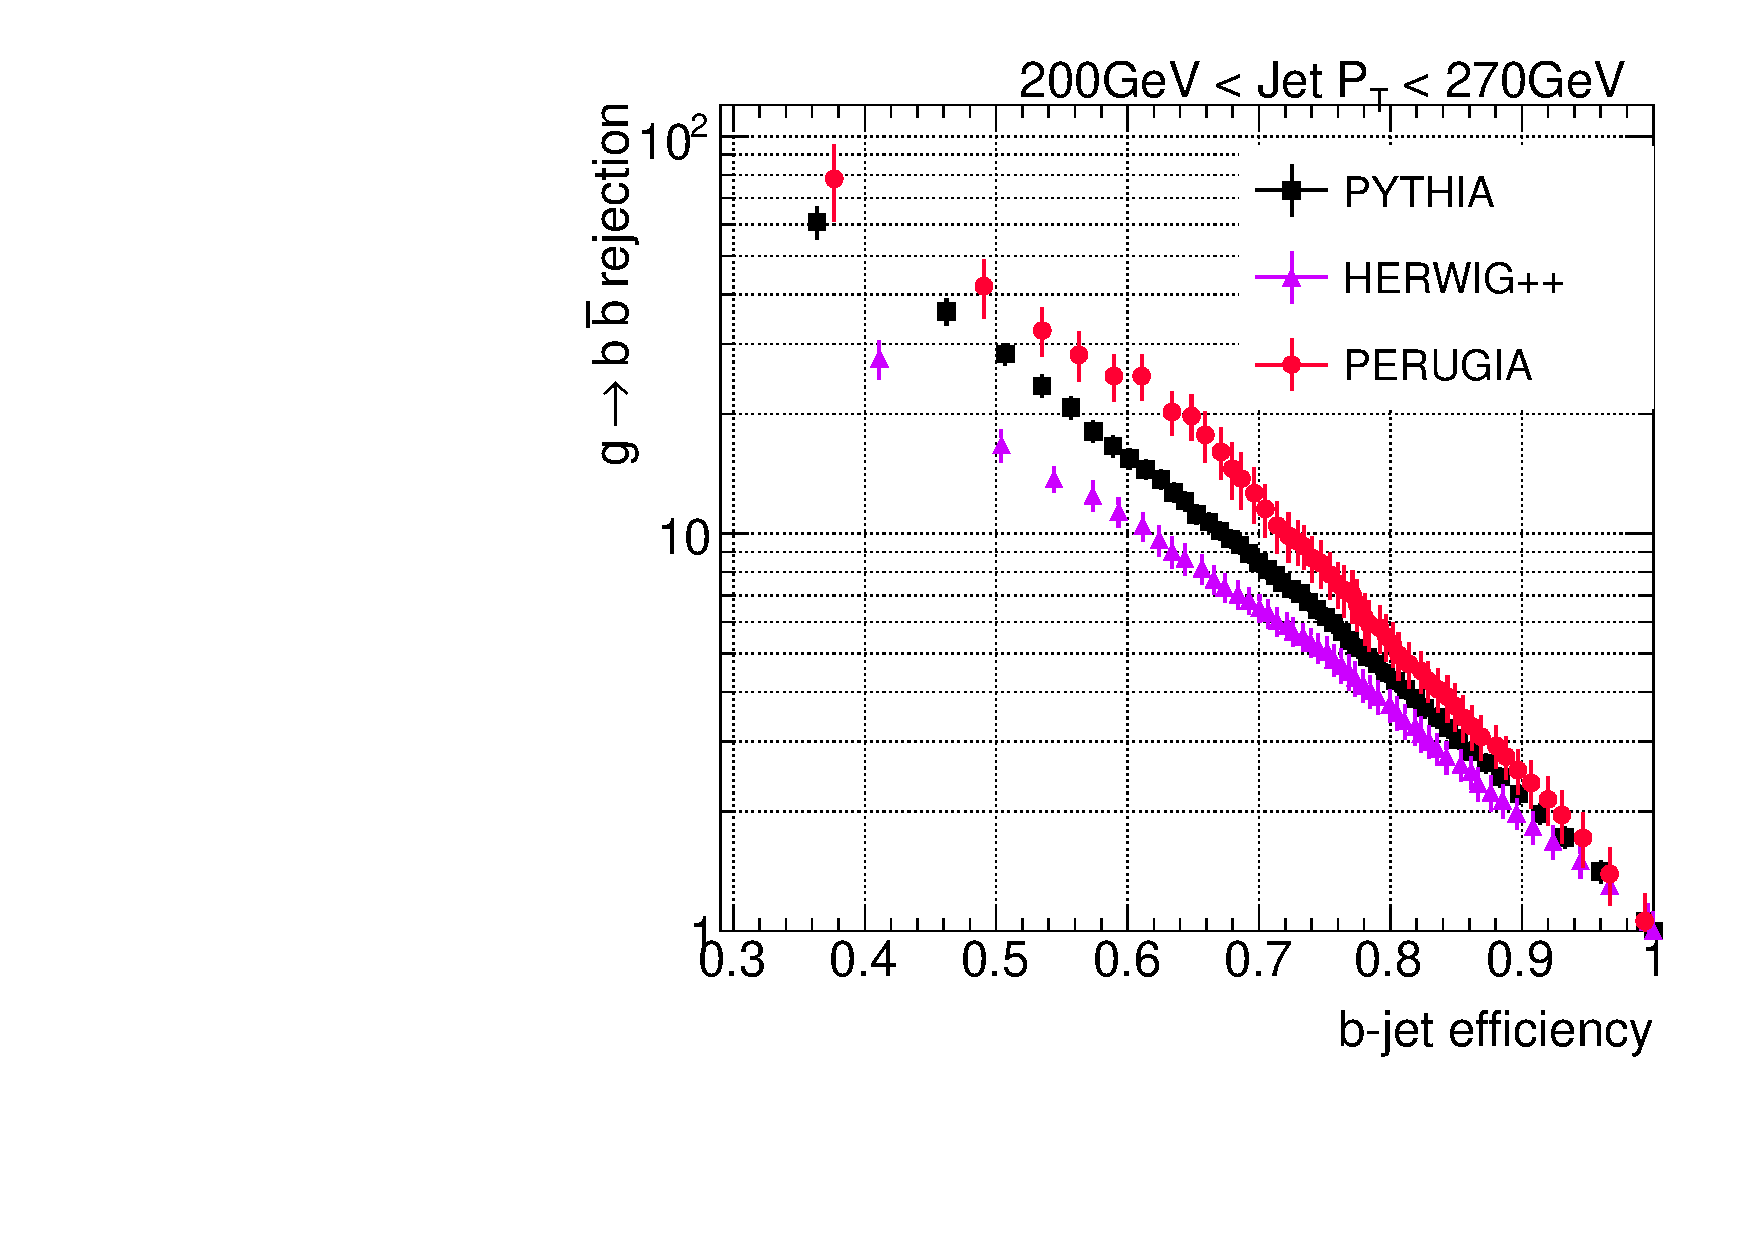
\includegraphics[width=0.49\textwidth]{FIGS/systematics/newInterpLlhoodKDE_ISO_DiffMCGen_rejvseff200.pdf}
%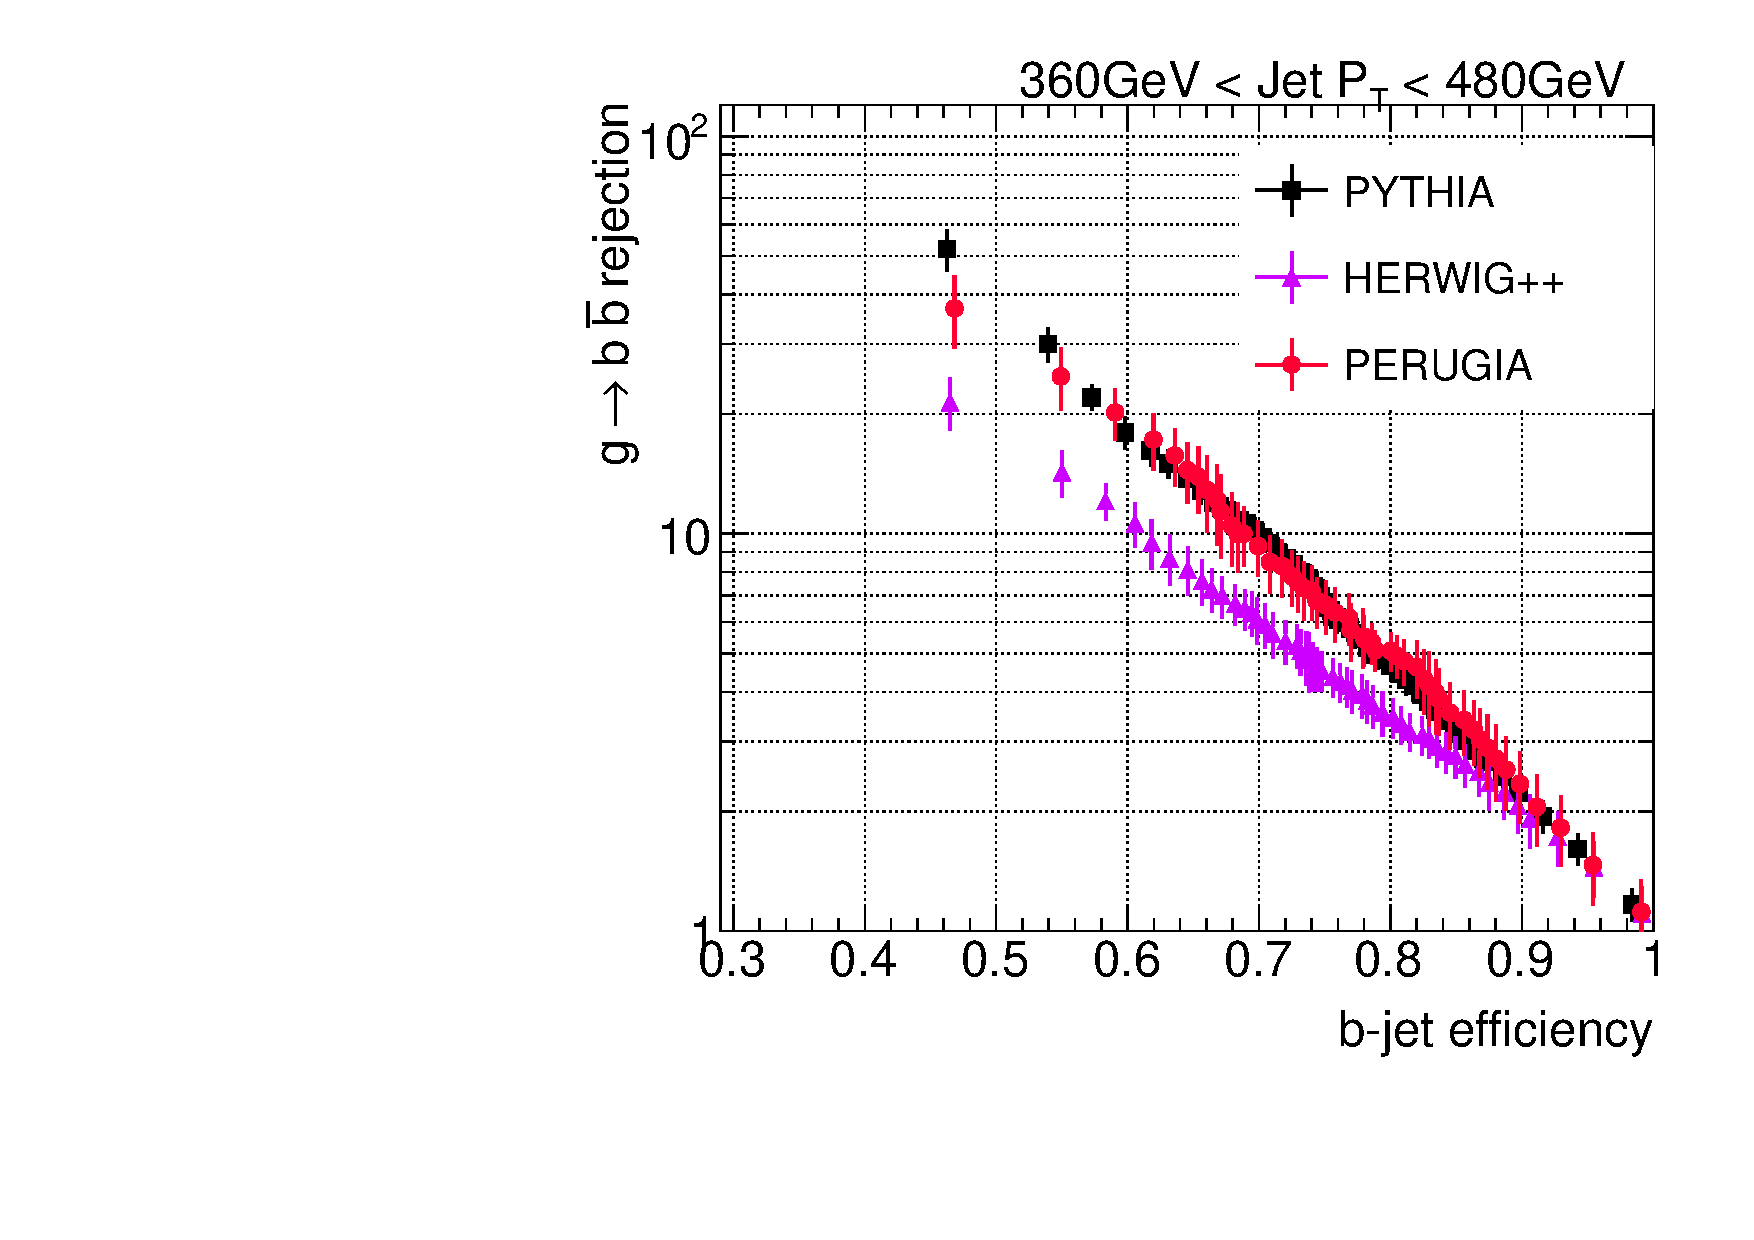
\includegraphics[width=0.49\textwidth]{FIGS/systematics/newInterpLlhoodKDE_ISO_DiffMCGen_rejvseff360.pdf}
\caption{Rejection of $g\rightarrow b \bar{b}$ merged $b$-jets as a function of jet $\pt$ for different Monte Carlo generators, at the 50\% efficiency working point.}
\label{fig:performanceotherMC}
\end{figure}

\begin{figure}[tp]
\centering
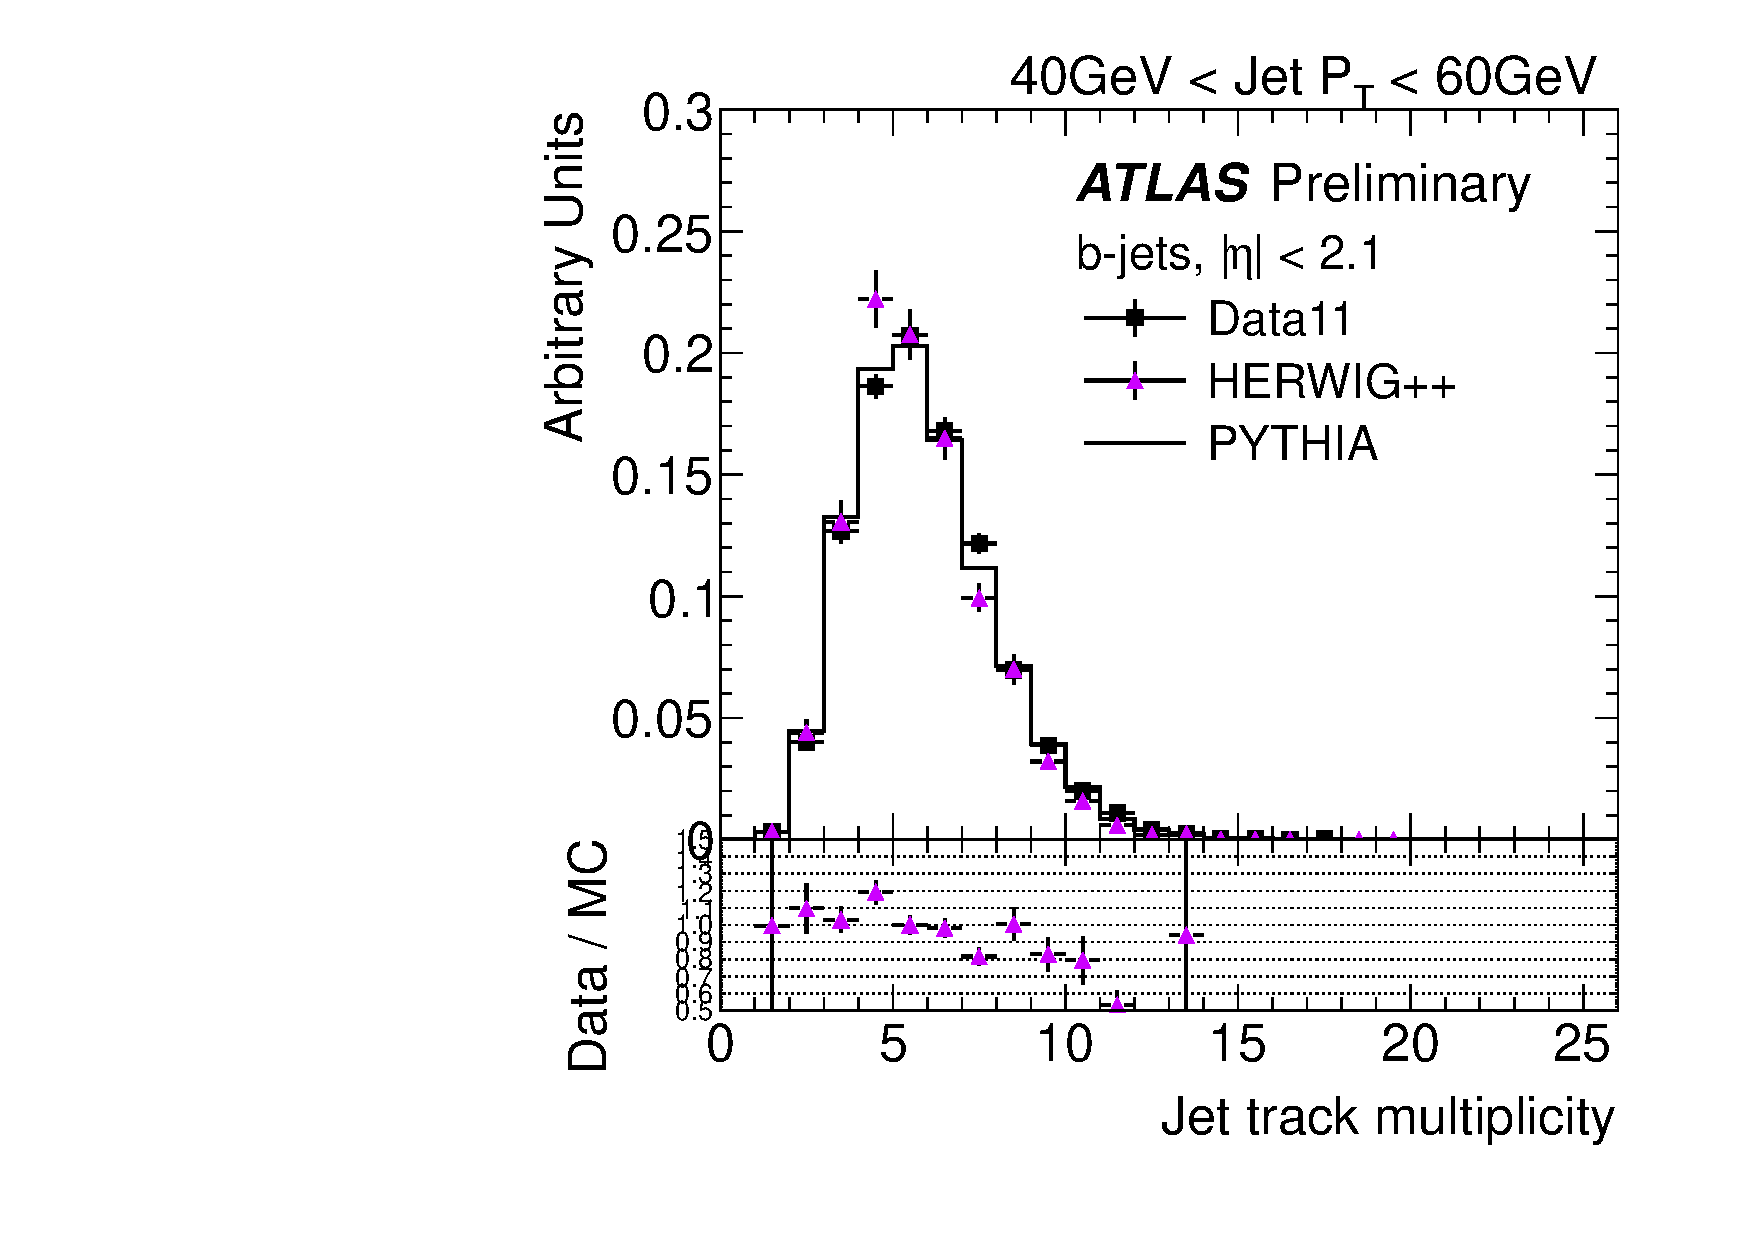
\includegraphics[width=0.49\textwidth]{FIGS/systematics/DataVarNtrkPT040.pdf}
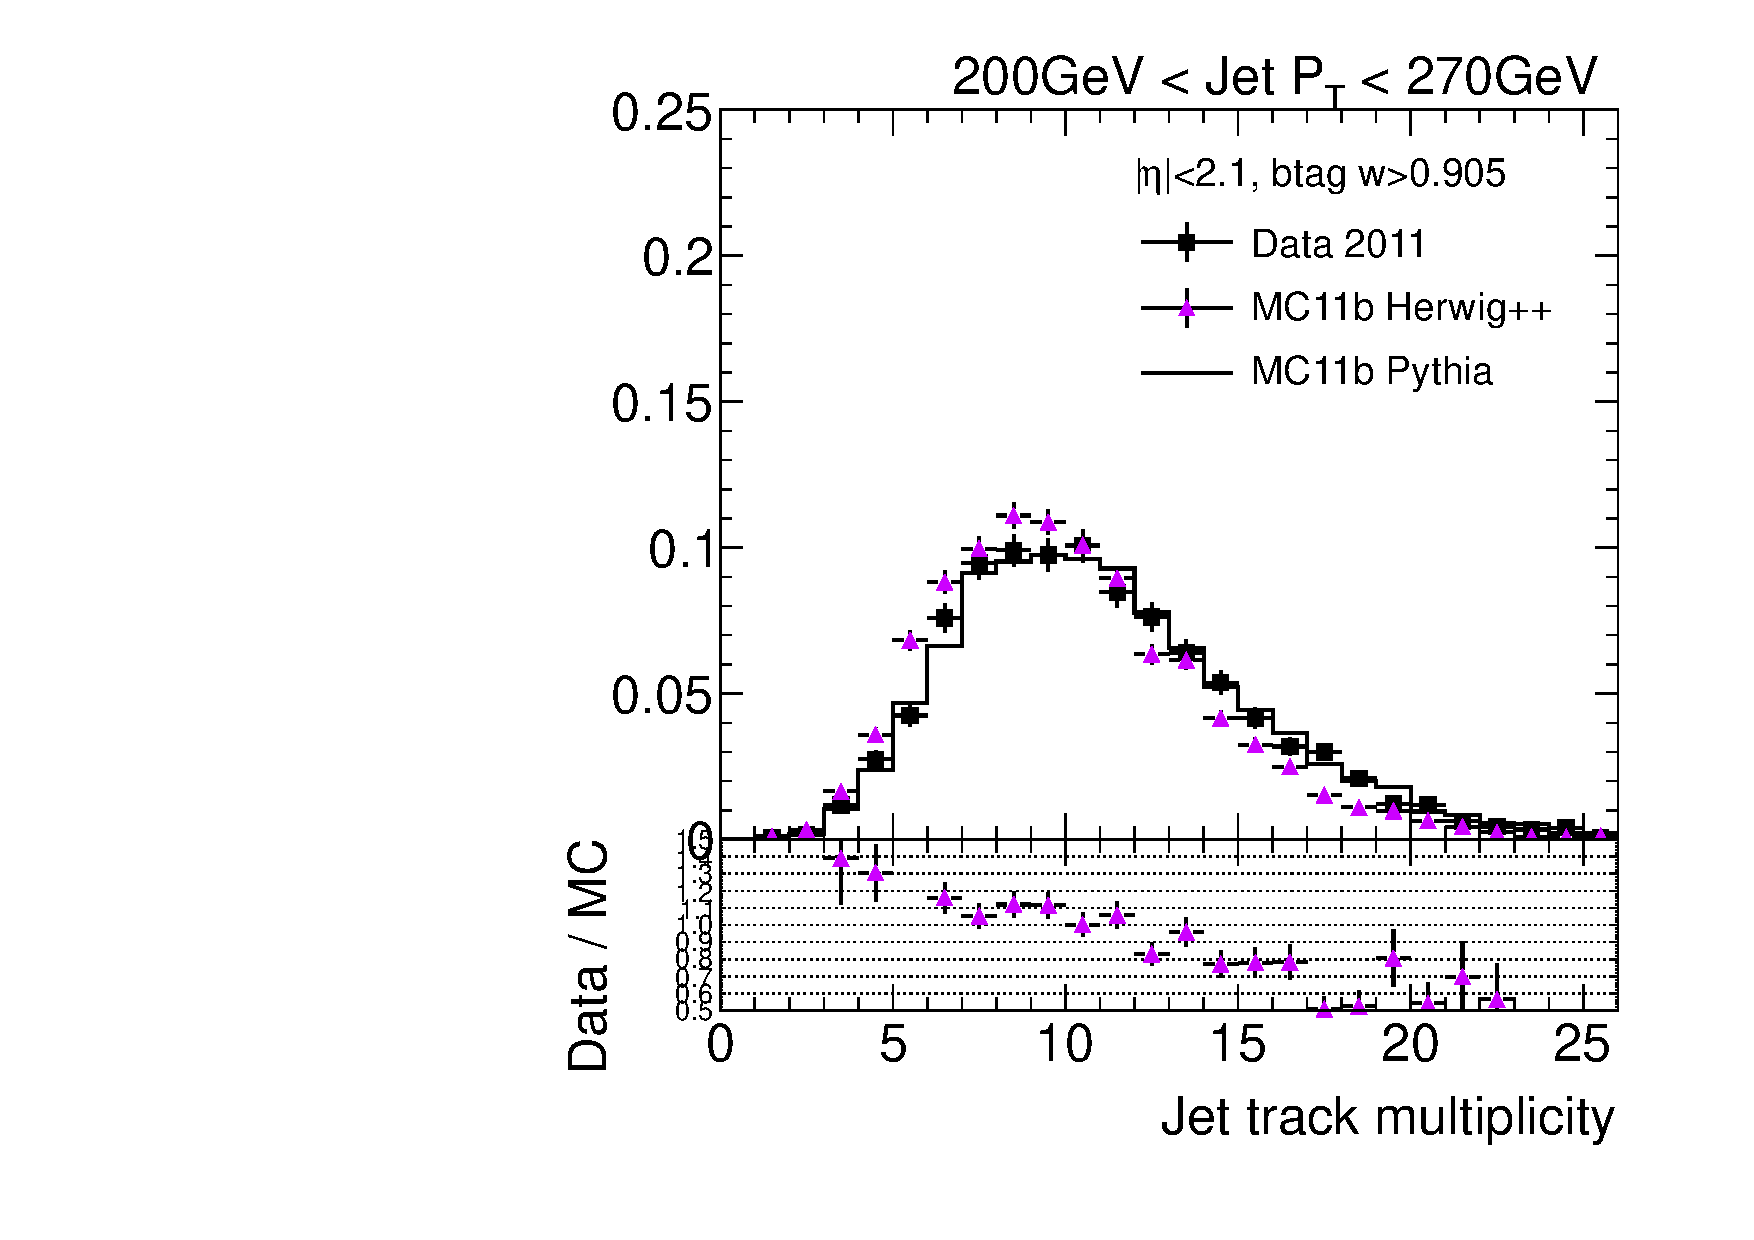
\includegraphics[width=0.49\textwidth]{FIGS/systematics/DataVarNtrkPT200.pdf}
\caption{Distribution of the jet track multiplicity in 2 different jet $\pt$ bins, for experimental data  collected during 2011 (solid black points) and {\sc herwig}++ events (solid violet triangules). The ratio data over {\sc herwig}++ simulation is shown at the bottom of the plot. {\sc pythia} distribution is also shown for reference.}
\label{fig:herwigdatamc}
\end{figure}



